%%% This is an example file for the Auburn University style options
%%%       aums.sty (Masters Thesis)
%%%       auphd.sty (Ph.D. Dissertation)
%%%       auhonors.sty (Honors Scholar)

%%%To use it, please edit the necessary options, title, author, date, year, keywords, advisor, professor, etc. 

\documentclass[12pt]{report}
\usepackage{aums}       % For Master's papers
\usepackage{ulem}       % underlining on style-page; see \normalem below
\usepackage{url}
\usepackage{tikz}
\usepackage{pgf}
\usepackage{tocloft}     % Use tocloft to introduce single spacing on long chapter name
\setlength\cftparskip{-2pt}
\usepackage[nottoc,notlof,notlot]{tocbibind} 
\usepackage{graphicx}
\usepackage{subcaption}
\usepackage{amsmath}
\usepackage{array}
\renewcommand\cftchapafterpnum{\vskip\baselineskip}  
\renewcommand\cftsecafterpnum{\vskip\baselineskip \normalfont}
\renewcommand\cftsubsecafterpnum{\vskip\baselineskip \normalfont}
\renewcommand\cftsubsubsecafterpnum{\vskip\baselineskip \normalsize}
\renewcommand\cftfigafterpnum{\vskip\baselineskip}
\renewcommand\cfttabafterpnum{\vskip\baselineskip}
\renewcommand{\cftpartleader}{\cftdotfill{\cftdotsep}} % for parts
\renewcommand{\cftchapleader}{\cftdotfill{\cftdotsep}} % for chapters
\usepackage{times}
\usepackage[a4paper,left=1in,right=1in,top=1.15in,bottom=1in]{geometry}
\usepackage{etoolbox}% http://ctan.org/pkg/etoolbox
\usepackage{titlesec}
\titleformat{\chapter}[display] %[display] puts the title chapter on a separate line
  {\singlespace\center}{\chaptertitlename\ \thechapter}{12pt}{\center} % Defines the Chapter title style and size
\titleformat*{\section} {\normalfont\fontsize{12}{12}}  % Added this line to describe section title,numbering and font styles
\titleformat*{\subsection} {\normalfont\fontsize{12}{12}}% Added this line to describe subsection title,numbering and font styles
\titleformat*{\subsubsection} {\normalfont\fontsize{12}{12}}% Added this line to describe subbsection title,numbering and font styles

%%%%%Format rules: Normal margins are 1 in. If you need to print with 1.5in margins, uncomment the line below
%\oddsidemargin0.5in \textwidth6in

%% If you do not need a List of Abbreviations, then comment out the lines below and the \printnomenclature line.
%%for List of Abbreviations information:  (see http://www.mackichan.com/TECHTALK/509.htm  )
\usepackage[intoc]{nomencl}
\renewcommand{\nomname}{List of Abbreviations}   	       
\makenomenclature 
%% don't forget to run:   makeindex ausample.nlo -s nomencl.ist -o ausample.nls
%% Also, if 




% May want theorems numbered by chapter
\newtheorem{theorem}{  \normalfont Theorem} [chapter]

% Put the title, author, and date in. 
\title{A Software Signal Simulation of Low Earth Orbit Satellites for Investigative Analysis}
\author{Samuel McDougal} 
\date{May 2023} %date of graduation
\copyrightyear{2023} %copyright year

\keywords{LEO Satellites, USRP, Navigation, Signals of Opportunity, Software Simulation, Signal Generation}

% Put the Thesis Adviser here. 
\adviser{Scott Martin}


% Put the committee here (including the adviser), one \professor for each. 
% The advisor must be first, and the dean of the graduate school must be last.
\professor{Scott Martin, PhD}

\professor{David Bevly, PhD}

\professor{Brendon Allen, PhD}

\begin{document}

\begin{romanpages}      % roman-numbered pages 

\TitlePage 

\begin{abstract} 
Simulation tools are an important part of the engineering design process by allowing changes in algorithms and processes before  implementation. Current global navigation satellite systems (GNSSs) are mainly located in medium Earth orbit (MEO) and have been used for many decades. GNSSs are used for positioning applications all across the globe from civilian to military applications. These satellite systems work well in most applications, however they are susceptible to interferences due to low signal power. Low Earth orbit (LEO) satellites have gained interest as a possible alternitive source of position, navigation, and timing (PNT). This is because LEO satellites have higher received signal power compared to standard GNSSs. One issue with LEO satellites is that the signal was not initially designed for navigation and most of the messages are unknown. 

This thesis describes the design of a software signal simulation tool for LEO satellites for investigative purposes. The tool is modular to allow for simulation blocks to be changed quickly and efficiently. This design also allows for new pieces to be written and integrated easily. The MATLAB simulation is capable of generating complex in-phase and quadrature signals for time division multiple access signals for current and hypothetical LEO constellations. The signals generated by this simulation tool are capable of being passed through a software receiver and through hardware by means of a universal software radio peripheral. By generating experimental signals, receivers can be designed and tested. To test the generated signals, a specialized receiver was designed. The output navigation data is used to produce position estimates for static receiver positions using batched Doppler and pseudorange based least squares algorithms. The simulation tool is shown to be flexible in order to examine varying test plans. 


\end{abstract}

\begin{acknowledgments}
I would first like to thank my wife, Madeline, for her immense amount of love and patience through this entire process. I know that it would have taken me the better part of a decade to finish this thesis if it was not for her. I would like to thank my family for all of their love and support and for always telling me to keep pushing forward. I would like to thank my friends in the GAVLAB for always willing to take a break from the school and work to go play a round of golf, play tennis, grab a bite to eat, or attend a sporting event. I would also like to thank Dr. Scott Martin and Dr. David Bevly for giving me the opportunity to attend Auburn University to earn my Master's degree. If I leave the reader with one piece of advice it would be that the juice is worth the squeeze. Earning a Master's degree is an incredible accomplishment and is worth all of the late nights and lack of sleep. The end goal is worth it. 
\end{acknowledgments}

\begin{singlespace}

\begin{center} 
\renewcommand{\cftchapfont}{}
\renewcommand{\cftchappagefont}{}
\renewcommand{\cfttoctitlefont}{\normalsize}% Remove \bfseries from ToC title
\renewcommand{\cftsecfont }{\normalsize}% Remove \bfseries from section titles in ToC
\renewcommand{\cftsecpagefont}{\normalsize}% Remove \bfseries from section titles' page in ToC
\tableofcontents 
\newpage
\renewcommand{\cftchapfont}{}
\renewcommand{\cftchappagefont}{}
\renewcommand{\cftloftitlefont}{\normalsize}% Remove \bfseries from lof title
\renewcommand{\cftsecfont}{\normalsize}% Remove \bfseries from section titles in lof
\renewcommand{\cftsecpagefont}{\normalsize}% Remove \bfseries from section titles' page in lof
\listoffigures
\newpage
\renewcommand{\cftchapfont}{}
\renewcommand{\cftchappagefont}{}
\renewcommand{\cftlottitlefont}{\normalsize}% Remove \bfseries from lot title
\renewcommand{\cftsecfont}{\normalsize}% Remove \bfseries from section titles in lof
\renewcommand{\cftsecpagefont}{\normalsize}% Remove \bfseries from section titles' page in lof
\listoftables
\end{center}
\end{singlespace}

\printnomenclature[0.5in] %used for the List of Abbreviations
\end{romanpages}        % All done with roman-numbered pages


\normalem       % Make italics the default for \em

 \chapter { Introduction}  % Use \\ for long titles  

\section { \normalfont Motivation}

Low Earth orbit (LEO) satellites for navigation have gained interest as an alternative source of position, navigation and timing (PNT) to GNSS due to GNSS being susceptible to interferences such as jamming, spoofing, and multipath. This is because the received signal power from LEO satellites is significantly larger than current GNSSs \cite{reidSatelliteNavigationAge2020}. Many current LEO satellites are not designed for navigation, however their signals have been exploited for opportunistic navigation. Many of these constellations have data messages that are unknown to the user which makes receiver design difficult. This can be combatted by designing a signal that is similar to the true signal. While there are a few high fidelity LEO simulators on the market, such as SimORBIT from Spirent, they can be expensive. Signal simulation tools allow for testing of signal types before satellites are launched. The development of a signal simulation tool that allows for testing of different signal types, satellite constellations, and receiver patterns is necessary for developing new LEO based GNSS applications, and software or hardware receivers for LEO satellites.

\section { Prior Work }

There are recent studies in positioning techniques with the growing interest in exploring navigation possibilities with LEO satellites. Currently, global navigation satellite systems (GNSSs) are an integral part of modern society. Whether it is directions to the grocery store, land surveying, or autonomous vehicles, the knowledge of the location and path of an object is important. Current GNSSs, such as Global Positioning System (GPS), use radio frequencies (RF) to determine position and velocity solutions. Methods for calculating positions and velocities from GPS satellites can be found in \cite{misraGlobalPositioningSystem2012}. 

The flexibility of a simulation tool is crucial. It saves time, money, and resources when testing different scenarios. One of the biggest advantages to the simulation tool proposed in this thesis is the ability to interchange different pieces quickly and efficiently. Whether it is the constellation type, data message, or signal structure, changes can be made easily to accommodate various test plans. Current navigation simulation tools,such as \cite{dongIFGPSSignal2003} and \cite{corbellDesignValidationAccurate2000}, are mainly focused on current GNSSs. A LEO signal simulator was designed in \cite{samuel_mcdougal_single-antenna_2022}. One source, \cite{powellMultipleAntennaSoftwareGPS} designs a signal simulation tool for ``Rapid Testing of Interference Mitigation Techniques" for GPS. In his thesis, Powell outlines structures for creating a low cost signal simulation tool that can be used to test different scenarios. He begins by generating a file of simulation settings. This is followed by a scenario simulation where satellites are propagated, measurements are generated, and the navigation message populated. Next the signal is generated for the satellites in view and the data is stored in a bin file. GNSS signal simulators can also be used to test software defined receivers (SDRs). Powell validates his simulation by comparing the generated signal performance to the performance of a hardware GPS receiver and examining the position, velocity, carrier to noise ratio, and Doppler frequencies. Powell found that the simulator described in his thesis was capable of producing realistic single and multi antenna signals. 


One of the main areas of research for LEO satellites is using the Doppler frequency measurements from the LEO satellites in order to compute a navigation solution \cite{hsuAssessmentUsingDoppler2014} \cite{psiakiNavigationUsingCarrier2021}. Doppler positioning has been used in GNSS \cite{bahramiGNSSDopplerPositioning}, and was even the precursor to GPS \cite{TransitSatelliteSpacebased}. The Transit satellite system was initially used for US naval ships to gain a rough position. In \cite{thompsonSingleDifferencedDoppler2021}, Thompson uses a double differenced Doppler technique to position a moving rover with LEO satellites using angle of arrival (AOA) estimates to remove the need of satellite state knowledge. The Argos satellite system uses Doppler measurements for animal tracking \cite{lopezImprovingArgosDoppler2014}
  

Another area of research pertaining to LEO satellites is the use of their measurements to collaborate with inertial measurement units (IMUs) for opportunistic navigation\cite{khalifeReceiverDesignDoppler2019}, \cite{tanNewMethodPositioning2019}. In \cite{moralesInertialNavigationSystem2018}, the Orbcomm constellation is used to to aid an inertial navigation system (INS) in a tightly-coupled fashion. Here they used the LEO satellite Doppler measurements and TLE files to estimate the position of a moving UAV without GNSS signals. For the experiment, the unmanned aerial vehicle(UAV) was without opperated without GPS and was required to use two Orbcomm satellites in view for navigation. They claim that this navigation framework lowered the UAV final position error by 72 percent when compared to solely using the IMU.

One possibility is to deploy a new constellation in LEO specifically for navigation  \cite{reidSatelliteNavigationAge2020}. Here Reid proposes a brand new constellation of LEO satellites that function similarly to current GNSSs. Reid claims that the positioning accuracy will be improved significantly due to higher received signal powers. The motivation behind the new constellation is to provide positioning accuracy for autonomous vehicles.

A LEO satellite signal simulator can be useful for testing different signal types, constellation geometries, and possible errors. While high end signal simulators exist, they can be expensive and require technical prowess to operate. A low cost version can be valuable and still operate at a high level of fidelity with more ease of use. 

\section { Contributions}
This thesis will describe the process of designing a modular simulation tool for LEO satellites. The versatility of the simulator allows the user to test different scenarios. 
The contributions from this thesis are listed below:
\begin{itemize}
    \item Description of LEO satellite signal simulation tool that generates realistic IQ signals to be used for currrent and experimental constellations
    \item Investigation of USRP playback and record to introduce hardware errors and prove the signal can be played into hardware
    \item Examine possible positioning techniques for TDMA signals
    
\end{itemize}

\section{Thesis Outline}
In Chapter 2, the background of satellite orbits, signal types, and modulation types are discussed. In Chapter 3, the simulation tool is described in detail. Chapter 4 dives into the simulation and testing configurations used for this thesis. The results from the testing configurations are discussed in Chapter 5. Conclusions and future work are discussed in Chapter 6 followed by a list of references and an appendix.


\chapter{Background}

\section{Satellite Based Navigation}\label{sec:satellitenav}
Satellite navigation employs trilateration as a way to solve the age-old problem of determining the location of ones self is on planet Earth. Trilateration is the process of using ranges to determine unknown locations of objects \cite{misraGlobalPositioningSystem2012}. In a two dimensional example seen in figure \ref{fig:Trilateration}, three transmitters produce circles with radius $r$. With knowledge of the location of the transmitters, the ranges can be used to calculate a circle around the transmitter. The intersection point of all three circles will enclose the positioning result.

\begin{figure}[h]
    \centering
    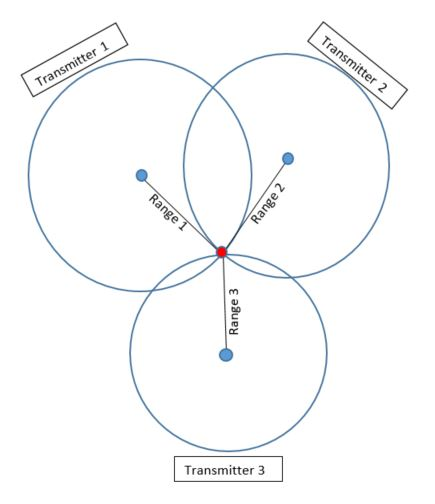
\includegraphics[width=4.0in]{Trilateration.JPG}
    \caption{Visual Depiction of Trilateration}
    \label{fig:Trilateration}
\end{figure}

The process of trilateration with satellites is the same except in three dimensional space. In the case of GPS, the satellites are the transmitters. Satellites make excellent transmitters in this case because of their ability to cover large areas continuously. An important point to mention is that in the previous example, it is assumed that the satellite and receiver are tied to the same clock. This means that the user has a perfect known time of the transmission of the signal from the satellite and perfect knowledge of the time of reception. This is not the case in real world examples. In fact, each satellite is tied to its own clock while each receiver is also tied to a separate clock. This offset in time can cause very large errors in positioning. To account for this, GPS ground stations survey and monitor the status of the satellite clocks to ensure maximum clock accuracy. While this takes care of the satellite part of the clock issue, the receiver clock still contains error. This error can be estimated along with the receiver states with the addition of a fourth measurement. With four unknown variables (receiver position $x$, $y$, $z$, and clock bias $b$), four measurements must be available in order to estimate the unknowns. 

Satellites use radio frequencies (RF) to transmit information to users on the surface of the Earth. These RF signals have encoded data called navigation messages that users can receive and unpack with specialized RF receivers. The navigation message can contain information such as satellite states, clock corrections, and orbital parameters. These parameters are used for obtaining the precise location of satellites to obtain ranges that are used for solving the positioning problem. 

\section{Satellite Orbit Zones}

With regard to space vehicles, there are three main orbital zones. These zones are low Earth orbit (LEO), medium Earth orbit (MEO), and geosynchronous Earth orbit (GEO). These zones are differentiated by the altitude of the orbit above the surface of the Earth. Due to the nature of the orbits, the satellites in these orbital zones have varying mission types. Figure \ref{fig:satorbzone} gives a reference to each of the orbital zones. 

\begin{figure}
    \centering
    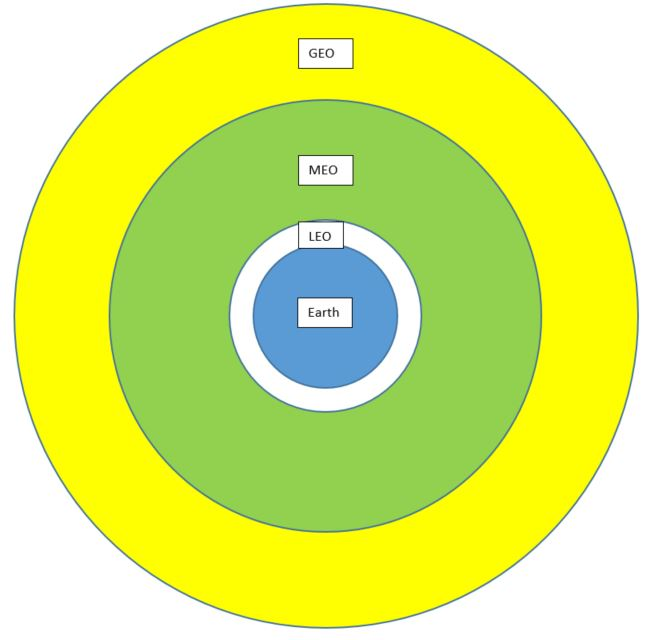
\includegraphics[width=4in]{satellite_orbit_zones.JPG}
    \caption{Visual Representation Orbit Zones}
    \label{fig:satorbzone}

\end{figure}

\subsection{Geosynchronous Orbit}
The furthest of the orbit zones is GEO. These satellites have an orbit altitude of 35,786 kilometers. Geosynchronous orbits are positioned at this precise altitude to allow the satellite orbit period to equal the same time as the rotation of the Earth for one day, also known as one siderial day. To an observer on Earth, the satellite would appear to stay in the same place throughout the course of its life. Another form of geosynchronous orbit is the geostationary orbit. Geostationary orbits are geosynchronous orbits specifically located at the Earth's equator and have a near zero inclination angle. 

One attribute of GEO satellites is that they have large footprints. The large footprint, along with twenty four hour coverage, means these satellites are useful for Earth observation, but not conducive for navigation. This also means fewer satellites are required to be in orbit for full Earth coverage. Many of the current GEO satellites are used for weather, climate surveying, and oceanic observations \cite{usdepartmentofcommerceSatellites}. The Geostationary Operational Environmental Satellites (GOES) are the current Earth observation satellites operated by NASA and NOAA \cite{garnerGOESOverviewHistory2015}. Since the orbit is so high, gaining a precise navigation message can be difficult due to loss of signal power and long signal transit times. Another issue with GEO satellites is the cost of launching these satellites. Launching satellites into GEO can carry a much higher price than satellites in LEO or MEO. These points were taken into consideration when GPS was first being designed \cite{misraGlobalPositioningSystem2012}.

\subsection{Medium Earth Orbit}
MEO is an orbital zone between LEO and GEO. MEO satellites have orbit altitudes between 2,000 kilometers and 35,000 kilometers. The orbit period for most MEO satellites is between 10 and 15 hours. Most of the satellites in MEO are navigation satellites which include GPS (USA), Galileo (European), GLONASS (Russia), and BieDou (China). Each country with GNSSs has designed them specifically for their own use. For example, GLONASS has an orbit altitude of 19,000 kilometers with satellites at specific inclination angles in order for the satellites to spend more time in view over Russia \cite{GLONASSInterfaceControl1998a}. GPS occupies MEO for many reasons, one being the number of satellites needed for global coverage. While more satellites are needed in MEO for global coverage than GEO, fewer are required than in LEO. GPS satellites have an orbit period near 12 hours. With their orbit altitude and orbit period, 24 satellites are needed for global coverage in order to have at least 4 satellites in view to gain a positioning solution.  

\subsection{Low Earth Orbit Satellites}
LEO satellites have orbits from 300 kilometers to 1500 kilometers. With this altitude, the orbit periods for LEO satellites are between 60 and 90 minutes. However, the amount of time that a satellite may be in view is lower. This poses issues in terms of global coverage. Satellite constellations with orbit periods on this time scale require far more satellites for full global coverage, and even more satellites for a possible navigation constellation. Reid et al says that it would take nearly 300 LEO satellites in order to provide global coverage \cite{reidSatelliteNavigationAge2020}. 

Current LEO constellations, such as Iridium and Orbcomm, are designed for communications. The Iridium constellation uses global coverage for satellite phones, where the Orbcomm constellation uses ``LEO satellites to provide worldwide geographic coverage for sending and receiving alphanumeric packages" \cite{orabiOpportunisticNavigationDoppler2021}. The data messages on these satellites are unknown as they are proprietary to the companies who deployed and opperate them. This makes it difficult to design receivers and evaluate the navigation performance of these signals. To address this issue a customized navigation message can be put on a similar signal. 

Current LEO constellations were not specifically designed for navigation. Most are used for satellite communications, internet, and Earth observations. Some of the major constellations in LEO are Iridium/IridiumNEXT, Orbcomm, and Starlink. IridiumNEXT \cite{IridiumNEXTReview2019}, which will be refered to as Iridium, is a telecomunications satellite network that is comprised of 66 active satellites and 9 in-orbit spares. The 66 active satellites are grouped into 6 orbital planes with 11 satellites in each plane. These satellites are in near polar orbits which means the coverage at the poles is very high, however coverage at the equator is low. The main mission for Iridium is to provide telecomunications with sat-phones. Orbcomm is similar to Iridium as it is a satellite communications constellation, however the physical constellation is different. 

Orbcomm has 48 satellites with varying inclination angles. The Starlink constellation is a satellite broadband internet provider \cite{Starlink}. This constellation utilizes LEO orbit in an effort to reduce latency with internet signals. Instead of using typical terrestrial based techniques for providing internet, satellites are used to give coverage in places where internet may not be readily available. However to accomplish this goal, a massive constellation of satellites must be deployed. Currently, there are nearly 3,600 Starlink satellites in LEO with more planned for launch. All of these constellations have one thing in common: the original purpose of their mission was not for navigation. 

\section{Channel Access Methods}

Channel access methods are ways of communicating through mediums between multiple devices by allowing users to send information back and forth between terminals and are used to manage telecomunications and wireless traffic. As there are multiple users trying to use or access the same information or services, channel access methods are used to differentiate between the users and the information being passed through the mediums. Three forms of channel access methods are time division multiple access (TDMA), code division multiple access (CDMA), and frequency division multiple access (FDMA). 

\subsection{Time Division Multiple Access}\label{sec:TDMAsection}

Time division multiple access signals use time to differentiate incoming signals. This results in the signal being burst-like in nature and non-continuous between received signals. The carrier frequency, however, can remain the same accross all users. TDMA signals are typically used by telecomunication satellites such as Iridium. These signals are ideal for communications because as the users are separated in time, the possibility of data interference between users is low. A visual representation of a TDMA signal can be seen in Figure \ref{fig:TDMAVisual}.

\begin{figure}[h!]
    \centering
    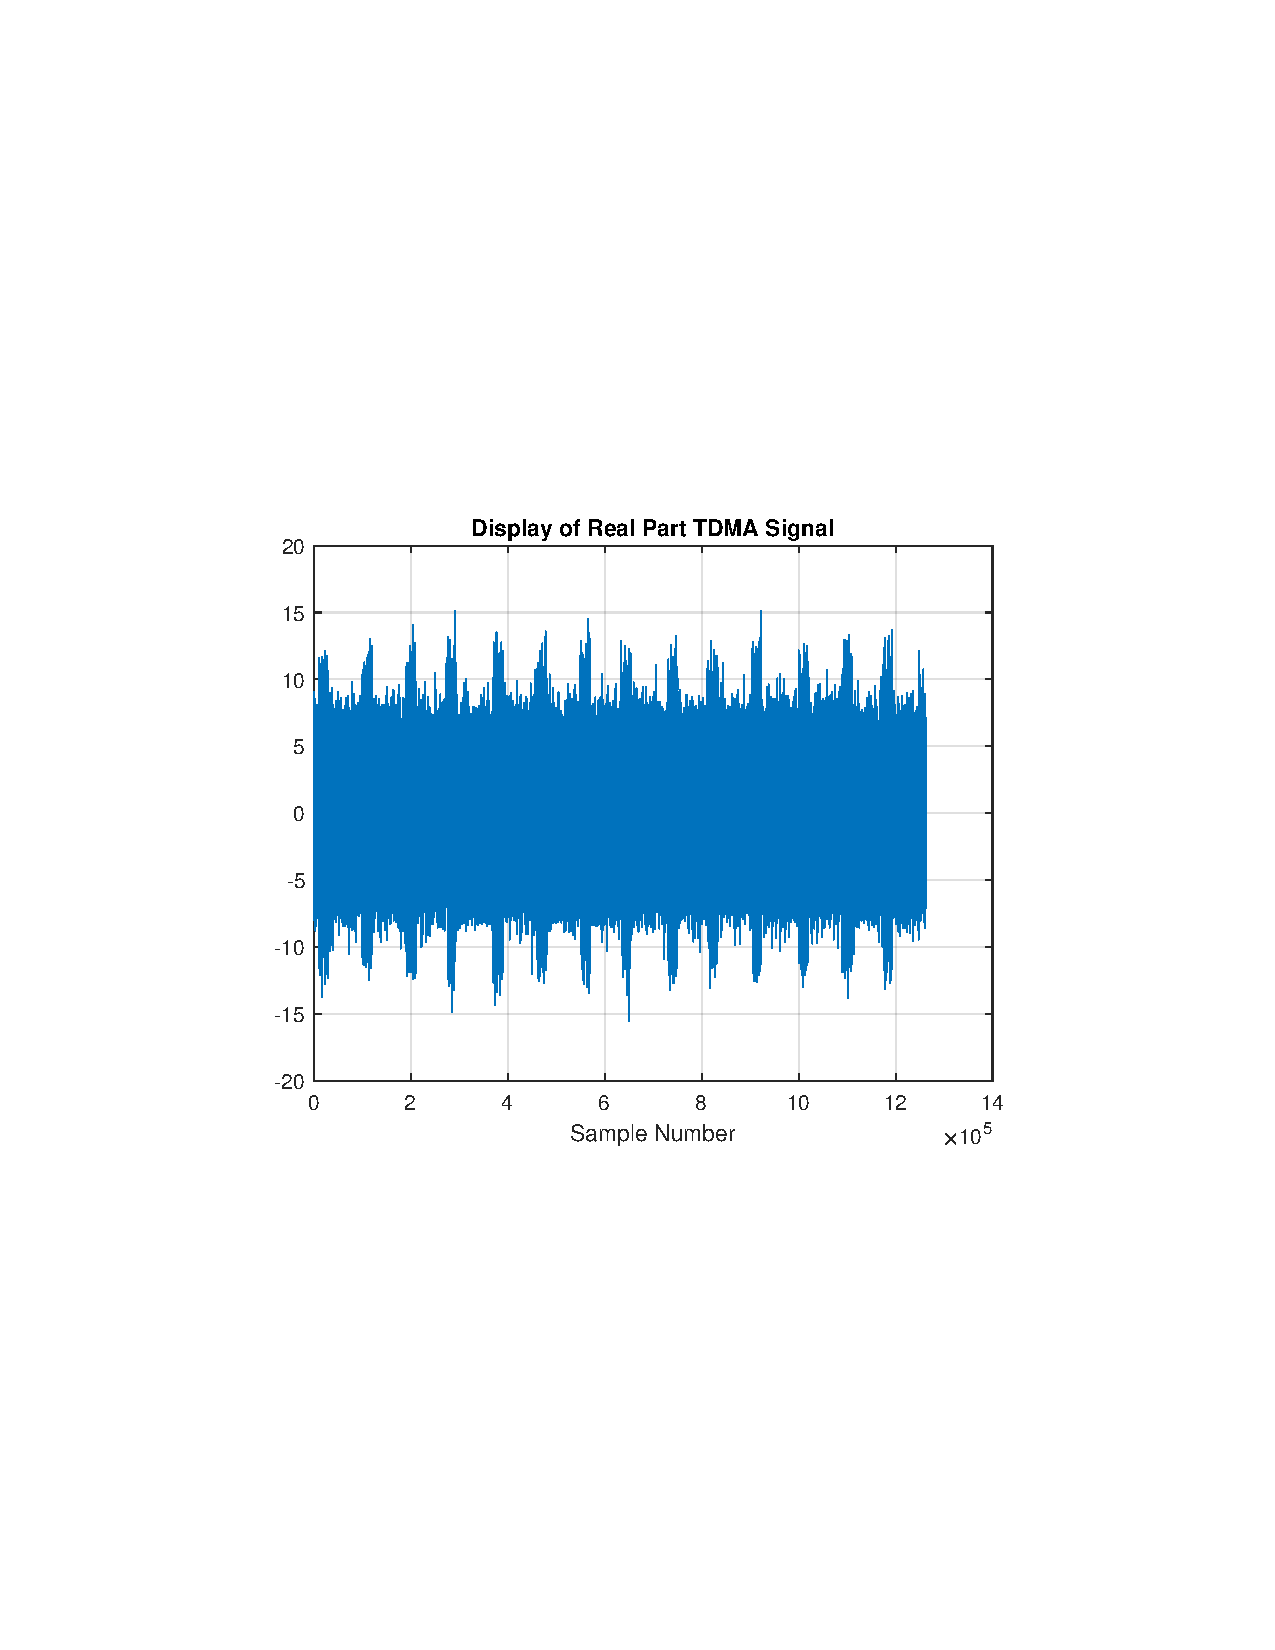
\includegraphics[width=5in]{TDMA_signal}
    \caption{Visual Representation of TDMA Signal}
    \label{fig:TDMAVisual}
\end{figure}

The burst nature of the signal can be seen in this image. The bulk of the signal is noise, and the parts extending out of the noise are the bursts. This shows the separation of the signal accross time. 

\subsection{Code Division Multiple Access}

Similar to TDMA, CDMA signals are broadcast at a single carrier frequency. However, unlike TDMA, CDMA signals use deterministic binary sequence codes to differentiate signals. In the case of satellites, each satellite is given its own pseudo-random noise (PRN) sequence. These codes are designed specifically to have very low cross correlation in order to eliminate errors and decipher different satellite's signals in the same frequency band. Cross correlation is a measure of similarity between two or more sequences. They also employ a high level of autocorrelation which is important for signal tracking \cite{goldOptimalBinarySequences1967}. Autocorrelation is a measure of how much a signal correlates with itself. Two notable GNSSs that employ CDMA signals are GPS and Galileo.

\subsection{Frequency Division Multiple Access}

Similar to CDMA, FDMA signals are continuous. However, these signals are not transmitted at the same carrier frequency. FDMA signals use different frequency bands to transmit data and information. For example, FM radio uses this technique to differentiate between radio channels such as sports talk radio and the local country music station. Similarly, some satellite constellations use the same concept to transmit data. For example, GLONASS uses FDMA signals for their satellites but also use a PRN code. Unlike GPS, however, they all transmit the same PRN sequence \cite{GLONASSSignalPlan}. 

\section{Modulation}
In the world of satellite navigation and telecommunications, the term modulation refers to the process of incorporating data onto a carrier wave. This data is represented in binary form through 1's and 0's. When a signal is generated, these ones and zeros are converted into 1's and -1's for the purpose of signal modulation. Three forms of modulation include amplitude shift keying (ASK), frequency shift keying (FSK), and phase shift keying (PSK). ASK is the process of changing the amplitude of the sine wave to represent ones and zeros of binary data, FSK is the process of changing the frequency of the sine wave to represent ones and zeros of binary data, and PSK changes the phase of the signal to incorporate the data. ASK and FSK are shown in Figures \ref{fig:ASKsig} and \ref{fig:FSKsig} respectively while two examples of PSK will be shown in the next section.

\begin{figure}[h]

    \centering
    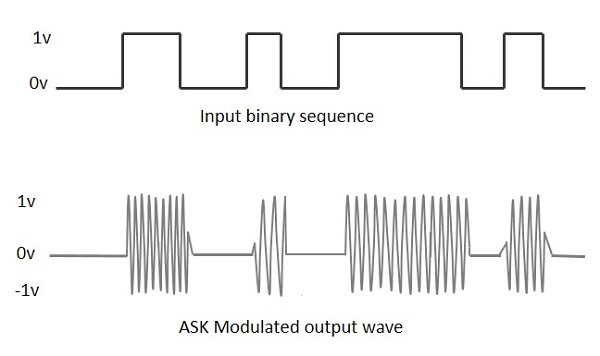
\includegraphics[width=4.5in]{ask_modulated_waveform.jpg}
    \caption{Amplitude Shift Keying Visualization \cite{AmplitudeShiftKeying} }
    \label{fig:ASKsig}

\end{figure}

\begin{figure}[h]

    \centering
    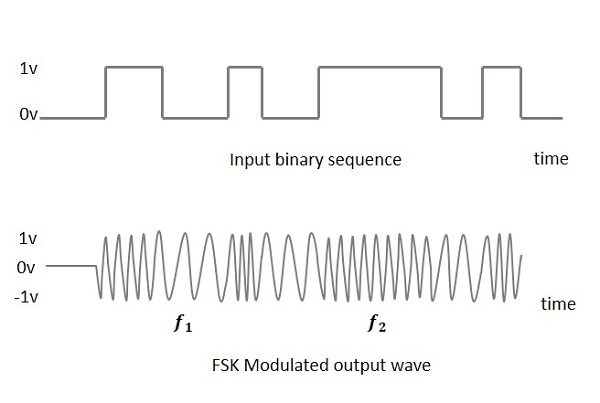
\includegraphics[width=4.5in]{fsk_modulated_output_wave.jpg}
    \caption{Frequency Shift Keying Visualization \cite{FrequencyShiftKeying} }
    \label{fig:FSKsig}

\end{figure}


\subsection{Binary Phase Shift Keying (BPSK)}

BPSK is accomplished by shifting the phase of the signal by 180 degrees depending on the sign of the data bit. By doing so, only one bit can be modulated per symbol. GPS uses BPSK modulation for its CA codes, navigation data, and P(Y) codes (encrypted message). BPSK is used due to its resiliance to bit error rate. A visual depiction of the BPSK signal can be seen in Figure \ref{fig:BPSKsig}. In the figure, the phase change of the signal by 180 degrees can be seen at the change of each data bit. 

\begin{figure}[h]
    \centering
    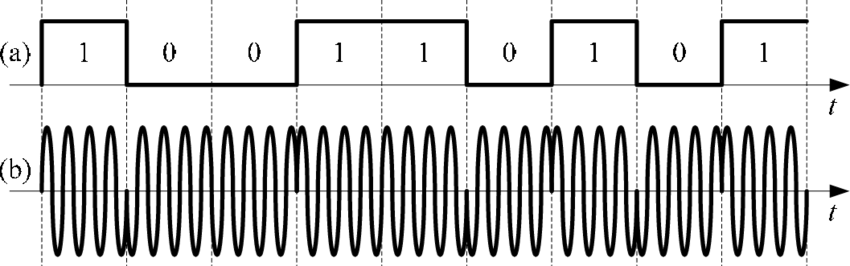
\includegraphics[width=4.5in]{Example-of-BPSK-modulation-format-a-binary-signal-and-b-BPSK-modulated-signal.png}
    \caption{Binary Phase Shift Keying Visualization \cite{mahdirajiAdvancedModulationFormats2010} }
    \label{fig:BPSKsig}
\end{figure}

\subsection{Quadrature Phase Shift Keying (QPSK)}
\label{sec:QPSK}

QPSK modulation uses 4 possible phases of the signal to modulate the data onto the carrier wave. The phase possibilities are 90 degree offsets. With this, two bits are transmitted in one symbol. This allows for faster data rates of the signal. Figure \ref{fig:QPSKmod} shows a visual example of QPSK modulation.

\begin{figure}[h]
    \centering
    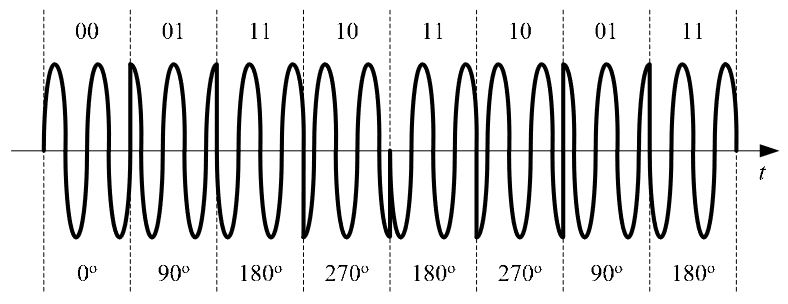
\includegraphics[width=4.5in]{QPSK_sig.JPG}
    \caption{Quadrature Phase Shift Keying Visualization \cite{mahdirajiAdvancedModulationFormats2010} }
    \label{fig:QPSKmod}
\end{figure}


\chapter {Simulation Tool}
In this section, the function and versatility of the simulator will be described.

\section{Simulator Overview}

The overall structure of the simulation is shown in Figure \ref{fig:SimDiagram}.

\begin{figure}[ht]
    \centering
    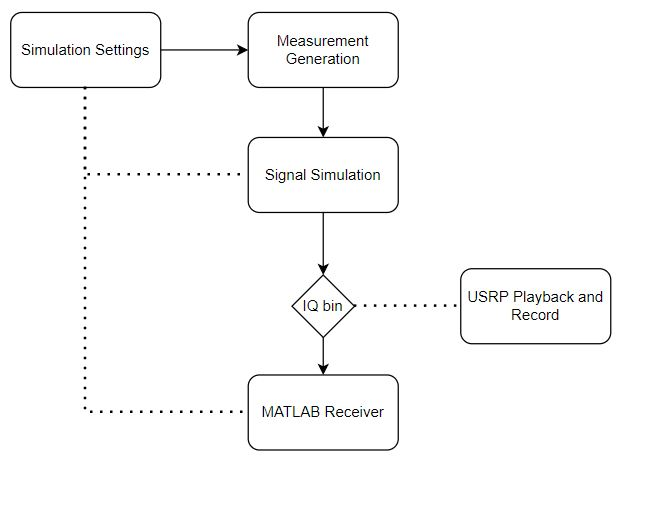
\includegraphics[width=6.0in]{OverallSimulationDiagram}
    \caption{Overall Simulation Diagram}
    \label{fig:SimDiagram}
\end{figure}

The simulation begins with the simulation settings file. This is a configuration file where all of the settings will be declared. This includes, but is not limited to, the satellite trajectories, signal power, and simulation length. The simulation settings file is fed into each section of the simulation tool. First, it goes into the measurement generation section. The measurement generation section is where the satellite positions and velocities are propagated, ranges and range rates are calculated, and transmit and received times are produced. Those terms are pushed into the signal simulation. Inside the signal simulation block the signal is generated and packaged into a bin file. Finally, the bin file is sent to a receiver where it is picked up, processed, and decoded to produce measurements. The following subsections will address each part of the simulation.

\section{Simulation Settings}

The simulation settings is a configuration file where all of the constants and settings used throughout the simulation are declared. All of the settings are stored in a MATLAB structure labeled `settings'. A MATLAB structure is a data storing type where sub-variables can be tied to one overall variable. The purpose of incorporating all of the settings and variables in one file is to ensure all variables are in one place. This helps the user find variables quickly and efficiently. It also aids the user by ensuring consistency across all parts of the simulation. 

In part, the simulation settings allow this tool to be modular. The file begins with constants such as the speed of light, rotation rate of the Earth, Earth gravitational constants, and time constants. These will likely stay the same across any and all simulations. Next is the input of user time. This time is in the format of year, month, day, hour, minute, second and determines the start time of the simulation. Following the time starting point is the duration of the simulation in seconds and the measurement simulation sampling frequency in hertz. The next setting is the user position. The simulation allows for static and dynamic receivers. For a static receiver an initial LLA position is declared, whereas the dynamic receiver will input the all positions in the Earth center Earth fixed (ECEF) coordinate frame. Next is the introduction of measurement error terms. The first set are weather terms for the error caused by the troposphere \cite{misraGlobalPositioningSystem2012}. These inputs are temperature in Celsius and Kelvin, barometric pressure in millibars, and humidity as a percentage. This is followed by clock settings. Here the user declares what type of clock to use and whether the clock error is to be simulated, indicated by an on or off switch. The clock is modeled based on \cite{brown_introduction_2012}. Next is the satellite propagation settings. This simulation uses a simplified general perturbation (SGP) model for calculating satellite positions and velocities. Here the user will input a two line element (TLE) file name along with other information used in parsing the TLE. The propagation settings also include a mask angle setting. The mask angle input is in degrees and allows the user to reject satellites under the specified elevation angle.
\begin{table}[hbt!]
    \centering
    \begin{tabular}{m{3cm} m{5cm} m{3cm} m{3cm}}
        \hline
        Section & Term & Variable & Units \\
        \hline
        \textbf{Time} & & & \\
        & Date & [Yr,Mo,D,h,m,s] &  N/A \\
        & & & \\
         & Sim Length & $t_{sim} $ & \textit{s} \\
         & & &  \\
         & Measurement frequency & $f_{sim}$ & \textit{Hz} \\
         \hline
         \textbf{User States} & & & \\
        & Position ECEF & \textit{x, y, z} & \textit{m}\\
         & Position LLA & ($L$, $\lambda$, $A$) & (\textit{deg},\textit{deg},\textit{m}) \\
         & & & \\
         & Velocity ECEF & ($\dot{x}, \dot{y}, \dot{z}$) & \textit{m/s} \\
         & Receiver Type & static/dynamic & 1/0 \\
        \hline
        \textbf{Satellite States} & & & \\
        & TLE File & & N/A \\
        & TLE Objects & & N/A \\
        & TLE Exclude Num. & & N/A \\
        & Augment Orbits & on/off & 1/0 \\
        & Augment Planes & N/A& \# \\
        & Augment Sats & N/A & \# \\
        & Augment Incl. & \textit{i} & \textit{deg.} \\
        & Augment Alt. & N/A & \textit{m} \\
        & Mask Angle & N/A & \textit{deg.} \\
        \hline
        \textbf{Error Terms} & & & \\
        Weather & Temperature & \textit{C,K} & \textit{deg.,deg.} \\
        & Barometric Pressure & $P_0$ & millibars \\
        & Humidity & N/A & \% \\
        & Trop. Toggle & N/A & on/off \\
        & & & \\
        Clock & Rec. Clock & Clock Type & N/A \\
        & Sat. Clock & Clock Type & N/A \\
        & Clock Toggle & on/off & 1/0 \\
        & & & \\
        Added Noise & N/A & $\epsilon$ & \textit{m} \\
        & Noise Toggle & on/off & 1/0 \\
        \hline
    \end{tabular}
        \caption{Measurement Simulation Settings}
        \label{table:measurementsimsettings}
\end{table}
\pagebreak

After the satellite propagation settings are the signal settings is Table \ref{table:sigsimsettings}. Here the user decides the carrier frequency, sampling frequency, code frequency, number of symbols in the data message, and signal type. Burst period and signal power are also declared. 

\begin{table}[hbt!]
    \centering
    \begin{tabular}{m{5cm} m{3cm} m{3cm}}
        \hline
        Term & Variable & Units \\
    \hline
        Carrier Frequency & $f_{carrier}$ & Hz \\
        Carrier Wavelength & $\lambda_{carrier}$ & \textit{m}\\
        Code Frequency & $f_{code}$ & Hz \\
        Symbols per Burst & N/A & \# \\
        Code Period & $T_{code} $ & \textit{s} \\
        Burst Length & $t_{burst}$ & \textit{s} \\
        Signal Noise Power & $P_{noise}$ & W, dB \\
        Carrier to Noise & CNo & dB-Hz \\
        Signal Power & $P_{signal}$ & W, dB \\
        Noise Toggle & on/off & 1/0 \\
        Generate Signal & on/off & 1/0 \\
        Data Message & Sv. States/COE & N/A \\
    \end{tabular}
    \caption{Signal Simulation Settings}
    \label{table:sigsimsettings}
\end{table}


The simulation settings file is integral to this simulation tool. All other components of this simulator are dependent on it. These specific dependencies will be explained in detail in the remaining subsections.

\pagebreak
\section{Measurement Simulation}
\subsection{Introduction}
The next block of the simulation tool is the measurement generation. The measurement generation is where satellites are propagated, ranges, range rates, and times are calculated. The purpose of this section is to have a set of truth values that will be used later in the simulation. The block diagram for the measurement generation is shown in figure \ref{fig:MeasBlock}.

\begin{figure}[h]
    \centering
    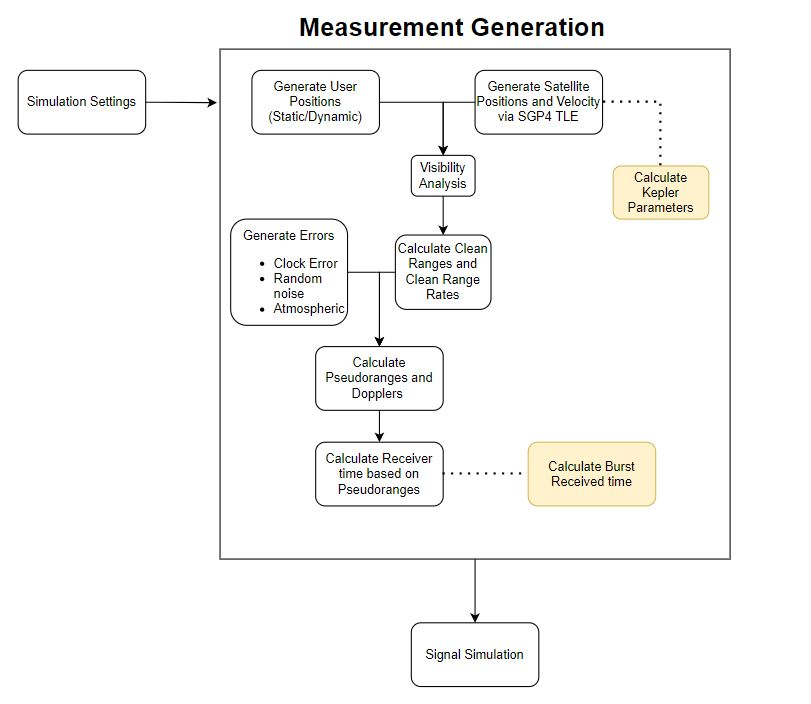
\includegraphics[width=6in]{MeasurementGenBlockDiagram}
    \caption{Measurement Generation Block Diagram}
    \label{fig:MeasBlock}
\end{figure}

The measurement simulation begins with the input of the simulation settings in Table \ref{table:measurementsimsettings}.A breakdown of the following subsections are as follows: satellite propagation, error generation, measurement calculation, and final outputs from the measurement simulation. 

\subsection{Satellite Propagation}
For this simulation tool satellites are generated using the SGP4 TLE propagator. SGP4 is a propagation technique used to calculate positions and velocities of satellites, space debris, and orbital junk. The SGP4 TLE propagator is used to calculate near Earth objects which are classified as having orbit periods less than 225 minutes. This corresponds well for LEO satellites as the orbital period is typically between 90 and 120 minutes. The perturbations accounted for in SGP4 include solar radiation, drag, and gravitational perturbations caused by the sun and the moon. SGP4 uses TLE files as a basis of propagation. TLE files are generated for tracking space objects. These files can be found on CelesTrak.org and can be pulled in the form of a text file for current day data. TLE files are 2 lines of 69 columns with orbital and satellite data. The information inside the TLE files is shown below.
\begin{table}
\begin{center}
    \begin{tabular}{|c|c|c|}
        \hline
        Columns Used & Term & Line Number \\
        \hline
        1 & Line number & 1 \\
        \hline
        3-7 & USSC satellite catalog number & 1 \\
        \hline
        8 & Classification & 1 \\
        \hline
        10-11 & Launch year & 1\\
        \hline
        12-14 & Launch number of year & 1 \\
        \hline
        15-17 & Part of launch & 1 \\
        \hline 
        19-20 & Epoch year & 1 \\
        \hline
        21-32 & Epoch day plus fractional & 1 \\
        \hline
        34-43 & Balistic coefficient & 1 \\
        \hline
        45-52 & Second derivative of mean motion & 1 \\
        \hline
        54-61 & B-star drag term & 1 \\
        \hline
        65-68 & Element Set number & 1 \\
        \hline
        69 & Checksum & 1 \\
        \hline\hline
        1 & Line number & 2 \\
        \hline
        3-7 & USSC satellite catalog number & 2 \\
        \hline
        9-16 & Inclination angle & 2 \\
        \hline
        18-25 & RAAN & 2 \\
        \hline
        27-33 & Eccentricity & 2 \\
        \hline
        35-42 & Argument of perigee & 2 \\
        \hline
        44-51 & Mean anomaly & 2 \\
        \hline
        53-63 & Mean motion & 2 \\
        \hline
        64-68 & Revolution number at epoch & 2 \\
        \hline
        69 & Checksum & 2 \\
        \hline\hline
    \end{tabular}
    \caption{Breakdown of TLE File Terms}
    \label{table:breakdowntle}
\end{center}
\end{table}

The TLE files found on CelesTrak.org are for current space objects and satellite constellations. 

The input settings for the This simulation tool are given in Table \ref{table:measurementsimsettings}. The TLE filename is name of the text file that houses the TLEs. The objects are the names of the satellites in the constellation. In some instances, there will be duplicates of satellites in a TLE file. These satellites need to be excluded when generating satellite data. This simulation tool includes the option to augment the pre-existing satellite constellations with more satellites. The options for the user are the number of orbital planes, satellites per plane, inclination angle, and orbit altitude. This feature is important for examining future constellations or investigating the performance of constellations that have not been conceived. The mask angle is declared in degrees. A mask angle is a term used to describe the the range of view that a receiver will receive a signal from. For example, if a receiver was in an open area, where the horizon is unobstructed, then the mask angle could be chosen to be zero degrees. However in most situations, the mask angle will be between 1 and 15 degrees. Additionally the length of the simulation and measurement sampling frequency are required for the propagation of satellites. A vector of predetermined receiver positions in the ECEF coordinate frame are included for the azimuth and elevation calculations. For a static the vector of user positions will remain the same through the simulation as the points are not changing in the ECEF frame. For a dynamic receiver the user will input a pre-recorded or generated path that has been sampled to the sampling frequency of the simulation.

The SGP4 TLE propagator begins with the input of the TLE file and the simulation settings. The TLE file is parsed and a MATLAB structure is used to store each element for each individual satellite. If declared the augmented satellite orbits are generated and added to the TLE structure. An Earth orientation parameters (EOP) file is hardcoded into the simulator, however this file needs to be updated periodically manually by the user. This data can also be aquired from the CelesTrak website. Time units are established and the begin time, end time, and time-step are calculated along with the time vector for the simulation. Memory is allocated for the position and velocity of each satellite in the ECEF and Earth centered inertial (ECI) coordinate frames.

Next the satellites are propagated one at a time for the length of the simulation. The position and velocity vectors are put into the respective preallocated variable for ECEF and ECI. The azimuth and elevation angle are calculated for each satellite at each timestep of the simulation using the satellite positions and user positions. The elevation angles will have values $-90^{\circ} < El < 90^{\circ}$. A visibility analysis can be performed with the elevation angles. The visibility analysis takes the elevation angles and finds the satellites that are above the mask angle to eliminate them from the simulation. The output of the visibility analysis is a list of satellites and the times that they are in view. This greatly reduces the computation time for the rest of the simulation because the simulator does not calculate measurements or signals for the out of view satellites. New variables of satellite positions and velocities are generated and filled for satellites that are in view. Mathematically this is represented in Equation \ref{eqn:VisAnal} where \textit{MA} is the mask angle and \textit{El} is the elevation angle.
\begin{equation}
    SV_{data} = 
    \left\{
        \begin{array}{lr}
            Fill cell, MA < El < 90^\circ \\
            NaN, MA > El
        \end{array}
    \right.
    \label{eqn:VisAnal}
\end{equation}
Each satellite state component ($x_{sv},y_{sv},z_{sv}$ and $\dot{x_{sv}},\dot{y_{sv}},\dot{z_{sv}}$) for both coordinate frames are saved into individual matrices. The dimensions for each matrix is $m \times n$, where \textit{m} is the length of the time vector and \textit{n} is the number of satellites propagated.
Figure \ref{fig:bothpropsats} shows the propagated satellite orbits in view above Auburn, Alabama for the Iridium and Orbcomm constellations over the duration of a 15 minute simulation. 

\begin{figure}[ht]
    \centering
    \begin{subfigure}{.4\textwidth}
        \centering
        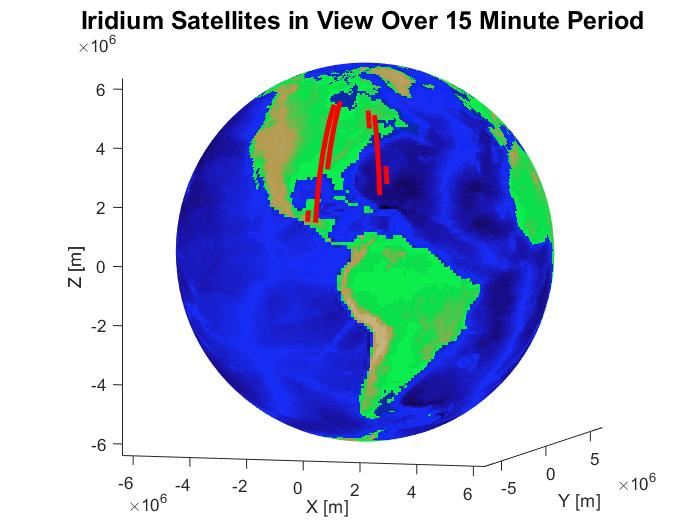
\includegraphics[width=\textwidth]{Iridium_sats_over_auburn.jpg}
        \caption{Propagated Iridium Satellites in View}
        \label{fig:IridSatsOverAub}
    \end{subfigure} %
    \begin{subfigure}{.42\textwidth}
        \centering
        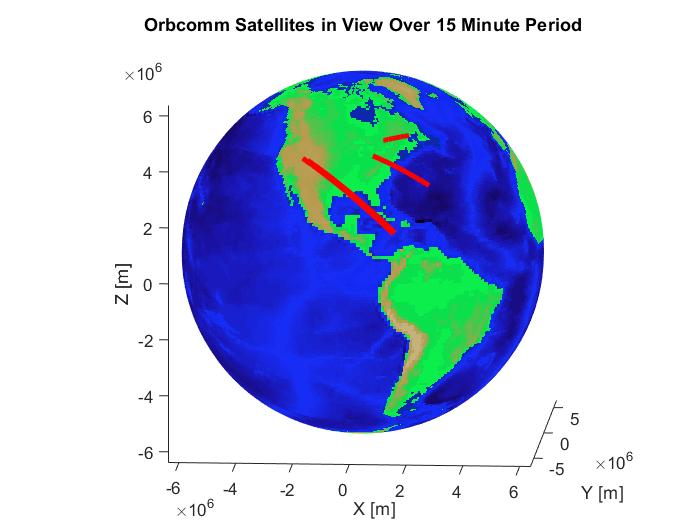
\includegraphics[width=\textwidth]{Orbcomm_sats_over_auburn.jpg}
        \caption{Propagated Orbcomm Satellites in View}
        \label{fig:OrbSatOverAub}
    \end{subfigure}
    \caption{Propagated Satellites from SGP4}
    \label{fig:bothpropsats}
\end{figure}

The final outputs from the satellite propagation stage are as follows:
\begin{description}
    \item[Satellite Positions] The 3-dimensional satellite position vectors in ECEF and ECI for all satellites propagated.
    \item[Satellite Velocity] The 3-dimensional satellite velocity vectors in ECEF and ECI for all satellites propagated.
    \item[Elevation Angle] The elevation angle of the satellites with respect to the user position.
    \item[In-view states] The 3-dimensional satellite position and velocity vectors in ECEF and ECI for in-view satellites.
\end{description}

With the satellites propagated and a visibility analysis conducted, the next step is to calculate errors.

\subsection{Error Generation}

After the visibility analysis, errors will be generated for the satellites that are in view. Measurement errors need to be calculated for computing the received time of the signal. Two primary sources of error modeled in this thesis are clock error and tropospheric delay. As previously discussed, clocks are imperfect and have a tendency to have a bias and drift over time due to the oscillator inside of the clock. For example, satellite clocks are more accurate because they use atomic clocks whereas receivers typically use a crystal oscillator. The tradeoff is cost. Atomic clocks are significantly more expensive than crystal oscillators. The satellite clock and receiver clock will have independent biases and drifts. The satellite is assumed to be capable of knowing and transmitting its bias and drift, while the receiver clock must be estimated by the receiver. Tropospheric delay is the error caused by gases in the Earth's atmosphere. The atmosphere is composed of dry gases and water vapor. These molecules have refractive properties that affect RF signals. The input settings for these errors are shown in Table \ref{table:measurementsimsettings}. The clock toggle switch is applied to the receiver and the satellites independently. The clock types described in Table \ref{table:ClockTypes} are declared. The error caused by the troposphere can be turned on or off with the toggle. The weather terms specified are the current weather states at the location of the receiver. 

The first error generated is clock error. The clock bias and clock drift are calculated for each satellite in view over the simulation based on the clock type described by the user. Next the receiver clock is modeled and the bias and drift are generated. These terms will be calculated based on \cite{brown_introduction_2012}. As previously mentioned, this option can be turned off and the errors will be incorporated as zeros in the simulation. The current clock types in the simulator are shown in the Table \ref{table:ClockTypes}. 

\begin{table}
\begin{center}
\begin{tabular}{|c c c c|}
    \hline
    Oscillator &  $\mathbf{h_0}$ & $\mathbf{h_{-1}} $ & $\mathbf{h_{-2}}$\\
    \hline\hline
    Cesium & $2 \times 10^{-22}$ & $5 \times 10^{-27}$ & $1.5 \times 10^{-33}$ \\
    \hline
    Rubidium & $2 \times 10^{-22}$ & $4.5 \times 10^{-26}$ & $1 \times 10^{-30}$\\
    \hline
    OCXO & $2 \times 10^{-25}$ & $7 \times 10^{-25}$ & $6 \times 10^{-25}$\\
    \hline
    TCXO & $2 \times 10^{-21}$ & $1 \times 10^{-22}$ & $3 \times 10^{-24}$\\
    \hline
\end{tabular}
\caption{Allan Variance Terms Used For Clock Error Generation}
\label{table:ClockTypes}
\end{center}
\end{table}

Next the tropospheric delay is calculated from the settings defined previously. The model used is found in \cite{misraGlobalPositioningSystem2012}. In this thesis the tropospheric delay is modeled as a function of elevation angle with the definition of obliquity factors. This is also refered to as mapping functions. The equation for tropospheric delay is 

\begin{equation}
    \tilde{T} = \tilde{T}_{z,d} \cdot m_d(el) + \tilde{T}_{z,w} \cdot m_w(el)
    \label{eqn:TropError}
\end{equation}
where $\tilde{T}_{z,d}$ and $\tilde{T}_{z,w}$ are the dry and wet tropospheric zenith delay, respectively, and $m_d$ and $m_w$ are the mapping functions for the dry and wet components. The Saastamoinen model is used for calculating the dry tropospheric zenith delay is calculated as

\begin{equation}
    \tilde{T}_{z,d} = 0.002277(1+0.0026cos2\phi +0.00028H)P_0
    \label{eqn:DryZenith}
\end{equation}
where $\phi$ is the latitude of the receiver, \textit{H} is the height of the receiver, and $P_0$ is the total pressure. 
The wet tropospheric zenith delay is calculated by Equation \ref{eqn:WetZenith} 

\begin{equation}
    \tilde{T}_{z,w} = 0.002277 \left( \frac{1255}{T_0} + 0.05 \right) e_0
    \label{eqn:WetZenith}
\end{equation}
where $T_0$ is the temperature in Kelvin and $e_0$ is the partial pressure due to water vapor.

The mapping function for the dry and wet delay can be seen in Equations \ref{eqn:drymapping} and \ref{eqn:wetmapping}, respectively.
\begin{equation}
    m_d(el) = \frac{1}{sin(el)+\frac{0.00143}{tan(el)+0.0445}}
    \label{eqn:drymapping}
\end{equation}
\begin{equation}
    m_w(el) = \frac{1}{sin(el)+\frac{0.00035}{tan(el)+0.017}}
    \label{eqn:wetmapping}
\end{equation}

Finally, white Gaussian noise is added for errors not modeled (i.e. Ionosphere delay, multipath, etc).

The final outputs of the error generation are as follows
\begin{description}
    \item[Satellite Clock Error] The error caused by satellite clocks. This is a MATLAB structure that is indexed for each satellite in view with fields of bias and drift. The error caused by bias and drift have units of meters and meters per second, respectively.
    \item[Receiver Clock Error] The error caused by the receiver clock. The receiver clock error is saved into the same structure as the satellite clock error labeled `ClockError'. The units for error caused by the bias and drift are also meters and meters per second, respectively.
    \item[Tropospheric Error] The error caused by the troposphere. This will be a matrix of tropospheric error for each satellite in view at each time step of the simulation. The unit for tropospheric is meters.
\end{description}

\subsection{Measurement Calculations}
With the errors generated, the measurements are calculated. The measurement calculations section only has one input from the simulation settings. This input is the burst timing of the signal. The user will declare this in terms of seconds. This step needs to be included because the receive time of the signal is calculated based on the satellite burst time. This will be discussed later in the section. This subsection will give the equations used for calculating true ranges and range rates, pseudoranges and pseudorange rates, Doppler frequency, and received time.

The true satellite to receiver ranges are calculated along with the range rates. Their equations are show below.
\begin{equation}
    r = \sqrt{(x^{(k)}_{sv} - x_u)^2 + (y^{(k)}_{sv} - y_u)^2 + (z^{(k)}_{sv} - z_u)^2}
    \label{eqn:rangeeqn}
\end{equation}
\begin{equation}
    \dot{r} = (\mathbf{v}^{k} - \mathbf{v}_r) \cdot \mathbf{1}
    \label{eqn:rangerate}
\end{equation}

Having generated ranges, range rates, and errors, the receiver observed pseudorange and Doppler measurements can be calculated. The equations for pseudorange, pseudorange rate, and Doppler are Equations \ref{eqn:pseudorange}, \ref{eqn:pseudorangerate}, and \ref{eqn:doppler}, respectively.

\begin{equation}
    \rho^{(k)} = r^{(k)} - b_{sv} + b_r + T +\epsilon
    \label{eqn:pseudorange}
\end{equation}
\begin{equation}
    \dot{\rho} = \dot{r} + \dot{b_r} - \dot{b_{sv}} + \epsilon
    \label{eqn:pseudorangerate}
\end{equation}
\begin{equation}
    f^{(k)}_{Doppler} = \frac{\dot{\rho}}{-\lambda}
    \label{eqn:doppler}
\end{equation}

Where in Equation \ref{eqn:pseudorange}, $\rho$ is the observed pseudorange calculated from range \textit{r} to the $k^{th}$ satellite, satellite clock bias $b_{sv}$, receiver clock bias $b_{r}$ in meters, troposphere delay \textit{T},  and additional noise for errors not modeled $\epsilon$. In Equation \ref{eqn:pseudorangerate}, $\dot{r}$ is the calculated range rate, $\dot{b_r}$ is the receiver clock drift, $\dot{b_{sv}}$ is the satellite clock drift, and un-modeled errors $\epsilon$, all with units of meters per second. In equation \ref{eqn:doppler}, $f^{k}_{Doppler}$ is the Doppler frequency of the $k^{th}$ satellite, $\dot{\rho}$ is the pseudorange rate, and $\lambda$ is the wavelength of the carrier. Once the pseudorange and Doppler measurements have been calculated, the observed received time of the signal can be calculated. It is important to calculate the received time of the signal based on the pseudorange because the signal is generated at the received level. The received time is calculated as 
\begin{equation}
    t_{rx} = t_{tx} + \frac{\rho}{c}
    \label{receivetime}
\end{equation}
where $t_{tx}$ is the transmit time, $\rho$ is the pseudorange calculated in Equation \ref{eqn:pseudorange}, and \textit{c} is the speed of light. For a TDMA signal, burst timing needs to be calculated. For example, if the burst timing 70 milliseconds, then a burst will occur at $t=0s$, $t=0.07s$, $t=0.14s$ and so on. For this instance, the received time of the signal is also calculated on the burst interval using Equation \ref{receivetime}.

An option the user has for a data message type is Kepler orbital parameters also known as classical orbital elements (COE). The calculation of COE uses the ECI satellite positions and velocities calculated previously. These terms are: \textit{h} magnitude of angular momentum; \textit{e} eccentricity; \textit{RAAN} right ascension of the ascending node, \textit{i} inclination angle; \textit{w} argument of perigee; \textit{TA} true anomaly; \textit{a} semi major axis. This process is described in \cite{curtisOrbitalMechanicsEngineering2008}.

The final outputs from the measurement generation are as follows:
\begin{description}
    \item[Satellite States] The positions and velocities of satellites that are in view for the duration of the simulation in meters and meters per second, respectively for both the ECEF and ECI frames. 
    \item[True Range] The true range of the satellite to the receiver in meters.
    \item[True Range Rate] The true range rate of the satellite to the receiver in meters per second.
    \item[Pseudorange] The calculated pseudoranges of the satellite to the receiver in meters.
    \item[Pseudorange Rate] The calculated pseudorange rate of the satellite to the receiver in meters per second.
    \item[Doppler Frequency] The calculated Doppler frequency in Hz.
    \item[Transmit Time] The transmit time of the satellites in seconds of simulation and in GPS time.
    \item[Received Time] The received time of the signal in seconds.
    \item[COE] Classical orbit elements that have been calculated for a possible data message.    
\end{description}

\section{Signal Simulation}
\subsection{Introduction}
The signal simulation begins directly after the measurement generation and is, naturally, where the signal is created. This simulation tool is for a QPSK TDMA signal as described in section \ref{sec:QPSK} and \ref{sec:TDMAsection}, respectively. Figure \ref{fig:SigSimBlock} gives an overview of the signal simulation. Inside the signal simulation the data message is generated and converted to binary data, received times are converted from seconds to samples, and signal noise is generated. Next the signal is generated, separated into real and imaginary parts, interleaved, and written to a bin file. The signal output will be a file of in-phase and quadrature (IQ) data.

\begin{figure}[h]
    \centering
    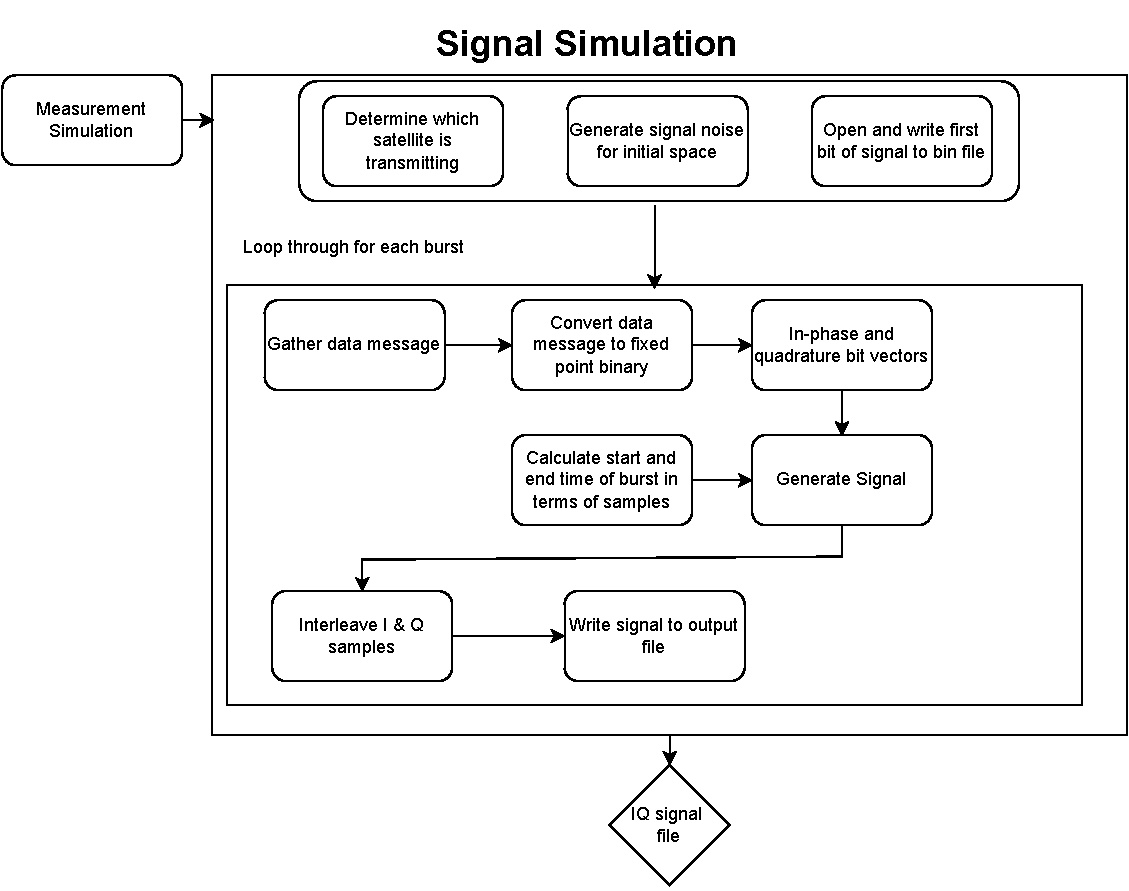
\includegraphics[width=5in]{Overall Simulation Diagram-Signal Simulation.drawio.pdf}
    \caption{Signal Simulation Block Diagram}
    \label{fig:SigSimBlock}
\end{figure}

The main settings used for the signal simulation are given in Table \ref{table:sigsimsettings}. The following subsections will procede as follows: initial calculations, data message generation, and signal generation.

\subsection{Initial Calculations}
Initial calculations that are made for the signal simulation. They are initial signal noise and satellite transmission determination. Since the simulation begins the transmission of a burst, an initial section of noise must be calculated. This is to account for the transmission time of the initial burst. Also, since only one burst occurs within the specified burst period, satellites must be chosen to transmit at specific times. 

The simulation starts by determining what satellite is transmitting and stores it into an array. This process is probabilistic and one satellite in view is chosen at random to transmit. This process is performed for each burst. Once the burst transmission list has been determined, the first part of the signal is generated. The first part of the output file will be signal noise. The signal noise will be the length of the first transit time in terms of samples. For example, if the first transit time is 0.003009 seconds and the sampling frequency is one megahertz, the first 3009 samples will be noise. Next a bin file is generated and signal noise is written to the file. 

\subsection{Data Message Generation}
The data message is a part of the signal used to gain information about the object transmitting the signal. For satellites, the data message is a package of numerical values representing the state of the satellite. This can be the satellite position and velocity, orbital elements, clock states, etc. With the calculated received times and designated satellites, the signal can be generated in blocks started by gathering the information for the data message. For this simulation, there are two options for a navigation message. The first option is to broadcast the satellite positions and velocities at the time of broadcast. The second option is to transmit the Kepler orbit parameters. Next, those terms are converted into fixed point binary strings. The data bits are generated in a separate function that is specific to the data message type. The length of each word is predetermined inside the data bit generation function.  The fractional length is determined based on the amount of precision the user desires. The decision to sign the word is also declared. The branch of in-phase or quadrature has also been predetermined. The outputs of the bit generation function are two row vectors of in-phase and quadrature bits. Non return to zero (NRZ) coding is used to represent the binary ones and zeros. Next, the number of samples in the signal block is determined by examining the begin time of the current burst and the begin time of the next burst. The difference in time is calculated and multiplied by the signal sampling frequency in order to calculate the number of samples in the block. Options for the data message types can be seen in Table \ref{table:SVPosDataMes} and Table \ref{table:COEdatMes}.

\begin{table}
\begin{center}
\begin{tabular}{|c|c|c|c|}
    \hline
    Term & Total bits & Fractional bits & Branch \\
    \hline
    Satellite ID & 8 & 0 & Q \\
    \hline
    Satellite Pos. & 32 & 7 & Q \\
    \hline
    Satellite Vel. & 32 & 7 & Q \\
    \hline
    Transmit Time & 64 & 0 & I \\
    \hline
\end{tabular}
\caption{Satellite Position and Velocity Data Message}
\label{table:SVPosDataMes}
\end{center}
\end{table}

\begin{table}
    \begin{center}
        \begin{tabular}{|c|c|c|c|}
            \hline
            Term & Total bits & Fractional bits & Branch \\
            \hline
            Sat ID & 8 & 0 & I \\
            \hline
            \textit{h} & 48 & 32 & Q \\
            \hline
            \textit{e} & 48 & 57 & Q \\
            \hline
            \textit{RAAN} & 48 & 45 & Q \\
            \hline
            \textit{i} & 48 & 47 & Q \\
            \hline
            \textit{w} & 48 & 47 & Q \\
            \hline
            \textit{TA} & 48 & 45 & Q \\
            \hline
            \textit{a} & 48 & 35 & Q \\
            \hline
            Transmit time & 48 & 17 & I \\
            \hline
        \end{tabular}
    \end{center}
    \caption{COE Data Message}
    \label{table:COEdatMes}
\end{table}
The satellite positions and velocities mentioned in Table \ref{table:SVPosDataMes} are for each individual cartesian component of the satellite position and velocity.

\subsection{Signal Generation}\label{sec:signalgen}
Next is the generation of the signal shown in Figure \ref{fig:SigGenBlock}. This is where all parts of the signal are combined together and generated. 

\begin{figure}[h]
    \centering
    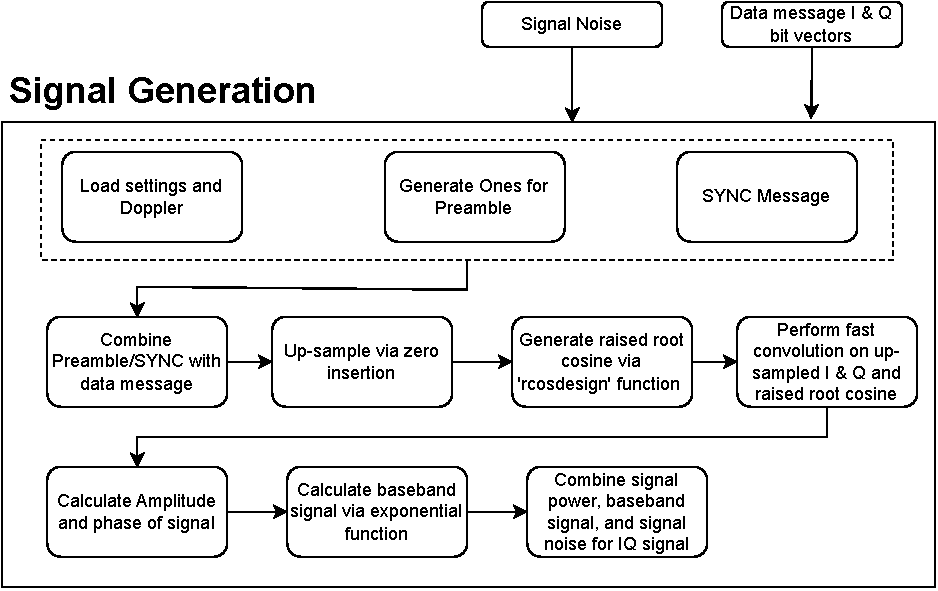
\includegraphics[width=5in]{Overall Simulation Diagram-Signal Generation.drawio.pdf}
    \caption{Signal Generation Block Diagram}
    \label{fig:SigGenBlock}
\end{figure}

The inputs to the signal generation block are signal power, sampling frequency, block size, Doppler frequency, signal noise, and the data message which has been converted into binary values.

A section of signal noise is generated for the amount of samples in the signal block. The sync message and preamble are a set of alphanumeric values that when converted to binary values have good autocorrelation properties \cite{dinanSpreadingCodesDirect1998}. The autocorrelation is important for the receiving and decoding of the signal and will be discussed further in this chapter. The preamble and sync messages are combined to their respective branches along with the in-phase and quadrature bit vectors to produce the full data message. If the number of bits used by the data message is lower than the number of bits in the burst, the remaining bits will be assigned random binary values. Up-sampling via zero insertion and filtering with a root-raised-cosine (RRC) pulse shaping filter is performed. The signal has to be up-sampled in order to meet the requirements set by the sampling frequency. The amplitude of the signal is calculated as Equation \ref{eqn:amplitude} and the phase is calculated in Equation \ref{eqn:phase}

\begin{equation}
    A = \sqrt{Ips^2 + Qps^2}
    \label{eqn:amplitude}
\end{equation}

\begin{equation}
    \theta = tan^{-1} \frac{Qps}{Ips}
    \label{eqn:phase}
\end{equation}
where \textit{Ips} and \textit{Qps} are the pulse shaped in-phase and quadrature branches respectively. The signal is generated through an exponential function in Equation \ref{eqn:signal}

\begin{equation}
    A e^{j2\pi (f_{Doppler}t + \theta)}
    \label{eqn:signal}
\end{equation}
where \textit{A} is the amplitude and $\theta$ is the phase. From here the declared signal power is added alongside the signal noise. The output of the generation function is a full IQ signal with, or without, noise. The signal is then split into real and imaginary parts, where they are interleaved and written to the bin file. To save computational memory, the signal variables are cleared with each iteration. This process is performed for each block of signal throughout the simulation. At the end of the simulation, if there is a received time outside the bounds of the simulation time, then the simulation will end the file with signal noise.

\subsection{Final Outputs}
The final outputs of the signal simulation are as follows:
\begin{description}
    \item[Bin file] A bin file with the generated signal where the real and imaginary parts of the signal have been interleaved.
    \item[I and Q bit matrix] A matrix with the in-phase and quadrature bit vectors of each burst are saved. These values are saved for analysis of bit rate error that will be observed in the results section of this thesis.
    \item[Navigation Data] A matrix of navigation data which includes the satellite number, satellite states, and transmit time for each burst is saved for analytical purposes.
\end{description}

\section{Receiver}\label{sec:receiver}
For this thesis, a specialized receiver was designed to process and verify the signal. It is based on the receiver in \cite{samuel_mcdougal_single-antenna_2022}. The purpose of a receiver is to take incoming RF data and process it into observables. These observables can be used to form a positioning solution. The inputs to the receiver are the binary data file, signal sampling frequency, sampling period, burst length, preamble-sync message, and burst time.

The receiver employs a matched filter. A matched filter is a way of detecting the signal by comparing it to a local replica of some part of the signal. In order to perform a matched filter some prior knowledge of the signal is necessary. In the case of this simulator the known part of the signal that remains constant across all bursts is the preamble and sync message. The preamble and sync message need to have good autocorrelation properties in order to perform the match filtering. With a local replica of the known preamble and sync message, bursts can be detected. Before burst detection can procede, a coarse frequency estimate must be obtained. This is because matched filters are low-pass filters. Since the incoming signal is pulse shaped, the bandwidth is lowered and creates a peak at the center frequency. This is used to estimate the Doppler frequency in Equation \ref{eqn:firstdopplerestimate}.

\begin{equation}
    f_d = argmax(R(f))
    \label{eqn:firstdopplerestimate}
\end{equation}
Here $f_d$ is the estimated Doppler frequency and $R(f)$ is the Fourier transform of the received signal. Next the Doppler frequency is removed by Equation \ref{eqn:dopplerremove}.
\begin{equation}
    r_{new}(t) = e^{-j2\pi f_d t} \times r(t)
    \label{eqn:dopplerremove}
\end{equation}
Where $r_{new}(t)$ is the new signal without the Doppler frequency and $r(t)$ is the input signal. This process is performed across the binary data file until the end of the file. The output of this is an estimate of the Doppler frequency, burst location, and burst number. The burst location comes from knowledge of the burst period and the peak discussed previously. The burst number is the sequential number of bursts detected. The burst location will be used later to calculate a pseudorange. 

Next, a raised root cosine (RRC) filter is used to filter the signal to raise the signal to noise ratio which helps with signal demodulation. An approximate symbol timing is used to provide a decimation period. The decimation period allows the received signal to be resampled at one sample per symbol. This is followed by removing residual frequency and phase. This is performed through a frequency and phase discriminator. The equation for the frequency discriminator is 

\begin{equation}
    f_{remaining} = \frac{atan2(cross,dot)}{t_2 - t_1}
    \label{eqn:freqdisc}
\end{equation}
where \textit{cross} and \textit{dot} are 
\begin{equation}
    cross = I_1Q_2 - I_2Q_2
\end{equation}
\begin{equation}
    dot = I_1I_2 + Q_1Q_2
\end{equation}
 $I_1$ and $Q_1$ are the sums of the first half of the tone and $I_2$ and $Q_2$ are the the sums of the second half of the tone. The remaining frequency can be wiped off by substituting $f_d$ with $f_{remaining}$ and $r$ with $r_{new}$ in Equation \ref{eqn:dopplerremove}. The phase is calculated as 
\begin{equation}
    \theta = atan2(Q/I)-\frac{\pi}{4}
\end{equation}
and the phase error is removed by 
\begin{equation}
    D(t) = e^{(j\theta)r(t)}
\end{equation}
where \textit{r(t)} is the post frequency discriminated signal and \textit{D(t)} is the output data bits.


Once the navigation bits have been demodulated they can be parsed and converted from binary values to full numerical values. The terms and values in Table \ref{table:SVPosDataMes} and \ref{table:COEdatMes} are used to obtain the location in the vector of bits each word occupies and how to convert back to numerical values. 

The final outputs of the receiver simulation are as follows:
\begin{description}
    \item[Decoded satellite data] The decoded navigation message of satellite number, satellite position, satellite velocity, and transmit time. If the chosen output is Kepler elements, the satellite positions and velocities will already be calculated.
    \item[Estimated Doppler] The estimated Doppler frequency from the receiver in Hz.
    \item[Range rate] The calculated range rate from the estimated Doppler frequency. 
    \item[Output bits] The output bits from the navigation message are saved to compare with the generated values.
    \item[Failed burst] This is a list of bursts that were observed, but the receiver failed to decode the data correctly.
    \item[Delta burst time] This is the change in time from previous burst. This term will be used to calculate a pseudorange for possible positioning. 
\end{description}

\chapter{Testing Setup and Positioning Techniques}
This chapter will discuss positioning techniques used for validation of results in this thesis. Two specific techniques examined are Doppler  and pseudorange based positioning. These techniques will be used along with the outputs of the receiver in order to gain a positioning solution.
 
\section{Doppler Based Positioning} \label{sec:DopplerPosTechnique}
Doppler positioning is not a new technique. In fact it was used with the original TRANSIT sytem in the 1960's and positioning accuracy was found to be within 500 meters. Doppler shift occurs as a result of a transmitter moving relative to an observer. As the transmitter moves closer, the frequency of the signal increases as the wave is being pushed closer to the observer. The opposite is true as the transmitter moves away from the user. The basis of Doppler positioning is using the change in signal frequency to gain an understanding of the motion of the transmitter. That information along with known satellite states can be used to gain a positioning solution.

The outputs of the receiver detailed in this thesis include the satellite position vector $\mathbf{r_{sv}}$, the satellite velocity vector $\mathbf{v_{sv}}$ and the received Doppler frequency $f_{Doppler}$. By rearanging Equation \ref{eqn:doppler}, the pseudorange rate of the $k^{th}$ satellite can be calculated in Equation \ref{eqn:prrfromdoppler}.

\begin{equation}
    \dot{\rho^{k}} = f_{Doppler}^{k} \cdot -\lambda
    \label{eqn:prrfromdoppler}
\end{equation}

Using \ref{eqn:prrfromdoppler} and \ref{eqn:rangerate} to rearange \ref{eqn:pseudorangerate}, the following equation is developed.

\begin{equation}
    \dot{\rho^{k}} = (\mathbf{v^{k}} - \mathbf{v_u}) \cdot \frac{(\mathbf{x^k} - \mathbf{x_u})}{\| \mathbf{x^k} - \mathbf{x_u}\|} + \dot{b} + \epsilon^{k}
    \label{eqn:extendedprreqn}
\end{equation}
For a static receiver $\mathbf{v_u}$ in Equation \ref{eqn:extendedprreqn} will be zero resulting in Equation \ref{eqn:staticextendedprreqn}.

\begin{equation}
    \dot{\rho^{k}} = \mathbf{v^{k}} \cdot \frac{(\mathbf{x^k} - \mathbf{x_u})}{\| \mathbf{x^k} - \mathbf{x_u}\|} + \dot{b} + \epsilon^{k}
    \label{eqn:staticextendedprreqn}
\end{equation}

With knowledge of the satellite states from the decoded navigation message, the unknowns are $\mathbf{x_u}$ and $\dot{b}$, where
\begin{equation}
\mathbf{x_u} = 
        [x_u \: y_u \: z_u]^T 
\end{equation}
With four unknowns, at least four measurements will be needed to solve for a positioning solution. An iterative process can be used to solve for the unknowns. 
First, an initial estimate of the states must be made. This will be represented by
\begin{equation}
    \mathbf{\hat{x}} = 
       [ \hat{x}_u \:
        \hat{y}_u \:
        \hat{z}_u \:
        \hat{\dot{b}}]^T
    \label{eqn:dopplerestimates}
\end{equation}
where $\mathbf{\hat{x}}$ is the vector of all unknown states, including the clock term.
Next is a vector of pseudorange rate measurements from \ref{eqn:prrfromdoppler} taking the form
\begin{equation}
\mathbf{\dot{\rho}} = 
    [\dot{\rho}_1 \:
    \dot{\rho}_2 \:
    \cdots \:
    \dot{\rho}_n]^T
\end{equation}
where $n$ is the number of measurements being used. Next an estimate of the pseudorange rate is calculated for each satellite by combining \ref{eqn:dopplerestimates} and \ref{eqn:staticextendedprreqn} to form 

\begin{equation}
    \mathbf{\hat{\dot{\rho}}} = \begin{bmatrix} 
        \mathbf{v_1} \cdot \frac{(\mathbf{x_1} - \mathbf{\hat{x_u}})}{\| \mathbf{x_1} - \mathbf{\hat{x_u}}\|} + \hat{\dot{b}} \\ 
        \mathbf{v_2} \cdot \frac{(\mathbf{x_2} - \mathbf{\hat{x_u}})}{\| \mathbf{x_2} - \mathbf{\hat{x_u}}\|} + \hat{\dot{b}} \\ 
        \vdots \\
        \mathbf{v_n} \cdot \frac{(\mathbf{x_n} - \mathbf{\hat{x_u}})}{\| \mathbf{x_n} - \mathbf{\hat{x_u}}\|} + \hat{\dot{b}} 
    \end{bmatrix}
    \label{eqn:pseudorangerateEstimate}
\end{equation}

The measurement matrix $\mathbf{H(\mathbf{\hat{x}})}$ is an $n \times 4$ matrix, where $n$ is the number of measurements being used.
\begin{equation}
\mathbf{H(\mathbf{\hat{x}})} = \begin{bmatrix}
    \frac{(\mathbf{x_1} - \mathbf{\hat{x_u}})}{\| \mathbf{x_1} - \mathbf{\hat{x_u}}\|} \times \left(\frac{(\mathbf{x_1} - \mathbf{\hat{x_u}})}{\| \mathbf{x_1} - \mathbf{\hat{x_u}}\|} \times \frac{\mathbf{v_1}}{\| \mathbf{x_1} - \mathbf{\hat{x_u}}\|}\right) && 1 \\
    \frac{(\mathbf{x_2} - \mathbf{\hat{x_u}})}{\| \mathbf{x_2} - \mathbf{\hat{x_u}}\|} \times \left(\frac{(\mathbf{x_2} - \mathbf{\hat{x_u}})}{\| \mathbf{x_2} - \mathbf{\hat{x_u}}\|} \times \frac{\mathbf{v_2}}{\| \mathbf{x_2} - \mathbf{\hat{x_u}}\|}\right) && 1 \\
    \vdots && \vdots\\
    \frac{(\mathbf{x_n} - \mathbf{\hat{x_u}})}{\| \mathbf{x_n} - \mathbf{\hat{x_u}}\|} \times \left(\frac{(\mathbf{x_n} - \mathbf{\hat{x_u}})}{\| \mathbf{x_n} - \mathbf{\hat{x_u}}\|} \times \frac{\mathbf{v_n}}{\| \mathbf{x_n} - \mathbf{\hat{x_u}}\|}\right) && 1 \\
\end{bmatrix}
\label{eqn:DopplerHMatrix}
\end{equation}
With this form, an estimate of the position and clock drift can be calculated using an iterative process. The first step of the process is input in Equation \ref{eqn:DopplerHMatrix} with the initial position guess, satellite positions, and satellite velocities. The next step is to calculate the pseudorange rates using Equation \ref{eqn:pseudorangerateEstimate} followed by calculating a delta pseudorange rate using Equation \ref{eqn:deltarangerate}.

\begin{equation}
\delta \mathbf{\dot{\rho}} = \mathbf{\dot{\rho}} - \mathbf{\hat{\dot{\rho}}}
\label{eqn:deltarangerate}
\end{equation}
By using the delta pseudorange rate, the error of the original estimate is what is being calculated. This is calculated through least squares shown in equation \ref{eqn:LeastSquares}.

\begin{equation}
\mathbf{\tilde{x}} = \mathbf{(H^TH)^{-1} H^T \delta \dot{\rho}}
    \label{eqn:LeastSquares}
\end{equation}
The new position estimate is calculated through \ref{eqn:NextEstimateIteration}.
\begin{equation}
    \mathbf{\hat{x}_{new}} = \mathbf{\hat{x}_{old}} + \mathbf{\tilde{x}}
\label{eqn:NextEstimateIteration}
\end{equation}
This process is continued iteratively until some threshold is met. Once the threshold is met, the process is concluded and the position and clock drift are output.

This process is typically employed using four or more measurements at the same time. For this thesis, a batched technique will be used. Since the nature of the signal used in this thesis is discontinuous, only one measurement is received at each time. One way to combat this is to use batched measurements. Batching measurements means taking measurements over a select period of time and treating them as if they are instantaneous. The advantage of batching measurements is that it allows the user to have enough measurements to compute an accurate position. Typically, when batching measurements, many measurements must be used in order to gain geometric diversity. One disadvantage of batching measurements is that it can take longer periods of time to gather enough measurements in order to gain a position estimate. The act of batching measurements is similar to averaging them over time. 

\section{Pseudorange Based Positioning} \label{sec:PseudorangePosTechnique}
Pseudorange based positioning is also not a new concept. Pseudoranges are used to solve the trilateration problem discussed in Section \ref{sec:satellitenav}. Equation \ref{eqn:pseudorange} previously discussed is the pseudorange equation. It includes the true range, satellite and receiver clock errors, atmospheric errors, and unmodeled effects. Similar to the Doppler positioning in Section \ref{sec:DopplerPosTechnique}, an iterative process is used to solve for a position solution. However instead of using the range rate, the pseudorange is used. There are a few modifications that need to be made to the equations used in this process, however the process of solving for the position as a whole is quite similar. 

First, the burst location in Section \ref{sec:receiver} is used to generate a pseudorange. A hot start is assumed in order to gain the first range to the satellite. A "hot start" means the initial position is known. The burst location can be used to calculate how much the pseudorange has changed between bursts. This is modeled as 
\begin{equation}
    \rho_{k}(t) = \rho_{k}(t-1) + \frac{(bl(t) - bl(t-1))}{f_s} \cdot c
    \label{eqn:pseudocalc}
\end{equation}
where \textit{bl} is the burst location in terms of samples, $f_s$ is the sampling frequency of the signal, and \textit{c} is the speed of light. This is performed for each satellite that has been received.

The pseudorange model to the $k^{th}$ satellite is 
\begin{equation}
    \rho_k(t) = r^k(t) + b_u(t) - b_s(t) + T(t) + \epsilon(t)
\end{equation}

where $r^k$ is the range to the satellite, $b_u$ is the user clock bias, $b_s$ is the satellite clock bias, \textit{T} is the error caused by the troposphere, and $\epsilon$ is the unmodeled error. The range from the user to the satellite is calculated as 

\begin{equation}
    r^k = || \mathbf{x^k - x_u}||
\end{equation}

where $\mathbf{x^k}$ is the three dimensional satellite position and $\mathbf{x_u}$ is the three dimensional user position. The Newton-Raphson method is used to estimate the user position and user clock bias. An initial guess of user position is the same as Equation \ref{eqn:dopplerestimates}. 
Next, the measurement matrix is formed 
\begin{equation}
    \mathbf{\hat{\rho}} = \begin{bmatrix} 
        -\frac{(\mathbf{x_1} - \mathbf{\hat{x_u}})}{\| \mathbf{x_1} - \mathbf{\hat{x_u}}\|} + \hat{\dot{b}} \\ 
        -\frac{(\mathbf{x_2} - \mathbf{\hat{x_u}})}{\| \mathbf{x_2} - \mathbf{\hat{x_u}}\|} + \hat{\dot{b}} \\ 
        \vdots \\
        -\frac{(\mathbf{x_n} - \mathbf{\hat{x_u}})}{\| \mathbf{x_n} - \mathbf{\hat{x_u}}\|} + \hat{\dot{b}} 
    \end{bmatrix}
    \label{eqn:pseudorangeEstimate}
\end{equation}

The delta pseudorange is calculated as 
\begin{equation}
    \delta \rho = \rho - \hat{\rho}
    \label{eqn:deltapseudo}
\end{equation}

The measurement matrix, \textit{H}, is 
\begin{equation}
    H = \begin{bmatrix}
        (-\mathbf{1^1}) && 1 \\
        (-\mathbf{1^2}) && 1 \\
        \vdots && \vdots \\
        (-\mathbf{1^k}) && 1
    \end{bmatrix}
\end{equation}
where $\mathbf{(1)}$ is the unit vector of satellite position and user position. 

The change in estimated position is calculated as 
\begin{equation}
    \begin{bmatrix}
        \delta \mathbf{x} \\
        \delta b
    \end{bmatrix}
    = (H^TH)^{-1}H^T\delta \mathbf{\rho}
\end{equation}

The next iteration of user position estimate is calculated as 

\begin{equation}
\hat{\mathbf{x}} = \mathbf{x_0} + \mathbf{\delta x}
\end{equation}

This process is solved iteritively until a threshold is met.

\section{Testing Setup}
The simulation is run in MATLAB as described at the begining of this thesis. The settings are declared, the measurements are generated, the signal is created, and the signal is processed by a software receiver. An additional step may be included where the signal is passed through a universal software radio periferal (USRP). The USRP demonstration is used to show that the signal generated in the simulation is capable of being passed through hardware. In this thesis an Ettus B200 mini USRP is used to perform a loopback function, shown in Figure \ref{fig:USRPsetup} where the signal is played through the USRP and recorded by the same USRP. 

\begin{figure}[h!]
    \centering
    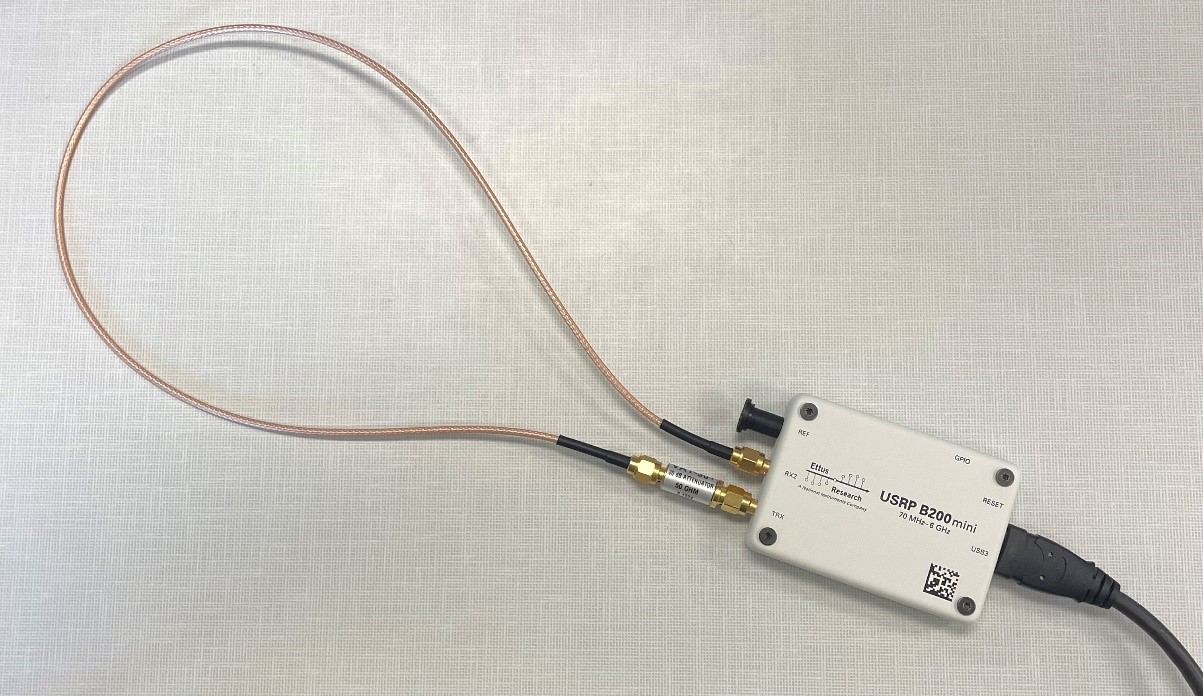
\includegraphics[width=5in]{USRP Setup.jpg}
    \caption{Ettus Research B200 Mini USRP Setup}
    \label{fig:USRPsetup}
\end{figure}

In order to do this, the generated signal cannot possess any errors. This is because the USRP will generate the errors on its own. The errors are background noise, transmitter clock error, and receiver clock error. The recorded signal is then passed through the software receiver for demodulation. This makes forming a position solution difficult and the results poor because the errors caused by the clock are unknown to the user. 

To show the versatility of the simulation tool, the following tests have been conducted.

\begin{itemize}
    \item Static receiver with no noise
    \item Static receiver played through USRP
    \item Static receiver with noise terms
    \item Static receiver with augmented satellites
    \item Dynamic receiver with no noise
\end{itemize}

\chapter{Results}

This chapter will be used to show the results from simulations run in this thesis. The purpose of these results is to show that the simulation tool is capable of producing a signal that gives realistic results. Five tests will be performed; they are a static receiver with no signal noise and no measurement noise, a static receiver where the signal has been played through a USRP, a static receiver with noise terms added, a static receiver with no noise and augmented satellites, and a dynamic receiver with no noise. 

While there are settings that will change between each simulation, some settings will remain constant. The sampling frequency of the measurements is 100Hz. The mask angle is set to 1.7 degrees. The code frequency is 25,000 Hz. The signal sampling frequency is 1 MHz. the burst length is 20.32 milliseconds. The burst interval is 90 milliseconds. The data message used in the signal is the ECEF position and velocity vectors of the satellites.

Figures and metrics used to show results will include geo plots of estimated receiver positions, root mean square error, and position dilution of precision (PDOP). PDOP is a measure of how good the positions of the satellites are for positioning. More diversity between satellite positions will result in a lower PDOP. Low PDOP values indicate the diversity of satellites is good for positioning. GPS satellites typically have a PDOP value lower than 2 \cite{misraGlobalPositioningSystem2012}. 

\section{Static Clean Data}
The data set generated for this scenario was a static receiver set with zero clock error, zero thermal signal noise, and zero atmospheric errors. The purpose of this experiment was to examine what the cleanest possible data set would produce. The position of the receiver was placed in Auburn, Alabama with a location of [32.602236,-85.489192,201] in LLA. The simulation length is 15 minutes. The constellation used is the IridiumNext constellation. 

For this data, the bit error rate of the decoded data is 99.07 percent for the in-phase branch and 99.087 percent for the quadrature branch. 

\subsection{Doppler Positioning}
The first positioning strategy for this data set is using the received Doppler measurements in a batched fashion using the equations in section \ref{sec:DopplerPosTechnique}. Figure \ref{fig:cleaniriddopgeo} shows the estimated receiver positions over the course of the simulation. The batch size for this was set at 2000 measurements. A few different batchh sizes were used, however below 2000 measurements the positioning error was greater due to less measurements, and above 2000 measurements the solution change was minimal. 

\begin{figure}[h!]
    \centering
    \includegraphics[trim=1.2in 3.3in 1.75in 3.3in,clip,width=5in]{Iridium Doppler Positioning from Cleanest Set.pdf}
    \caption{Position Estimate from Batched Doppler Measurements}
    \label{fig:cleaniriddopgeo}
\end{figure}
The RMS positioning error is shown in Figure \ref{fig:RMSErrorBatchDoppler}. The error in the Doppler positioning is caused by the error induced by the software receiver. In the software receiver, the Doppler frequency is estimated to a degree of +/- 50 Hz. This combined with the satellite geometry and batching of measurements causes the error shown. 

\begin{figure}[h!]
    \centering
    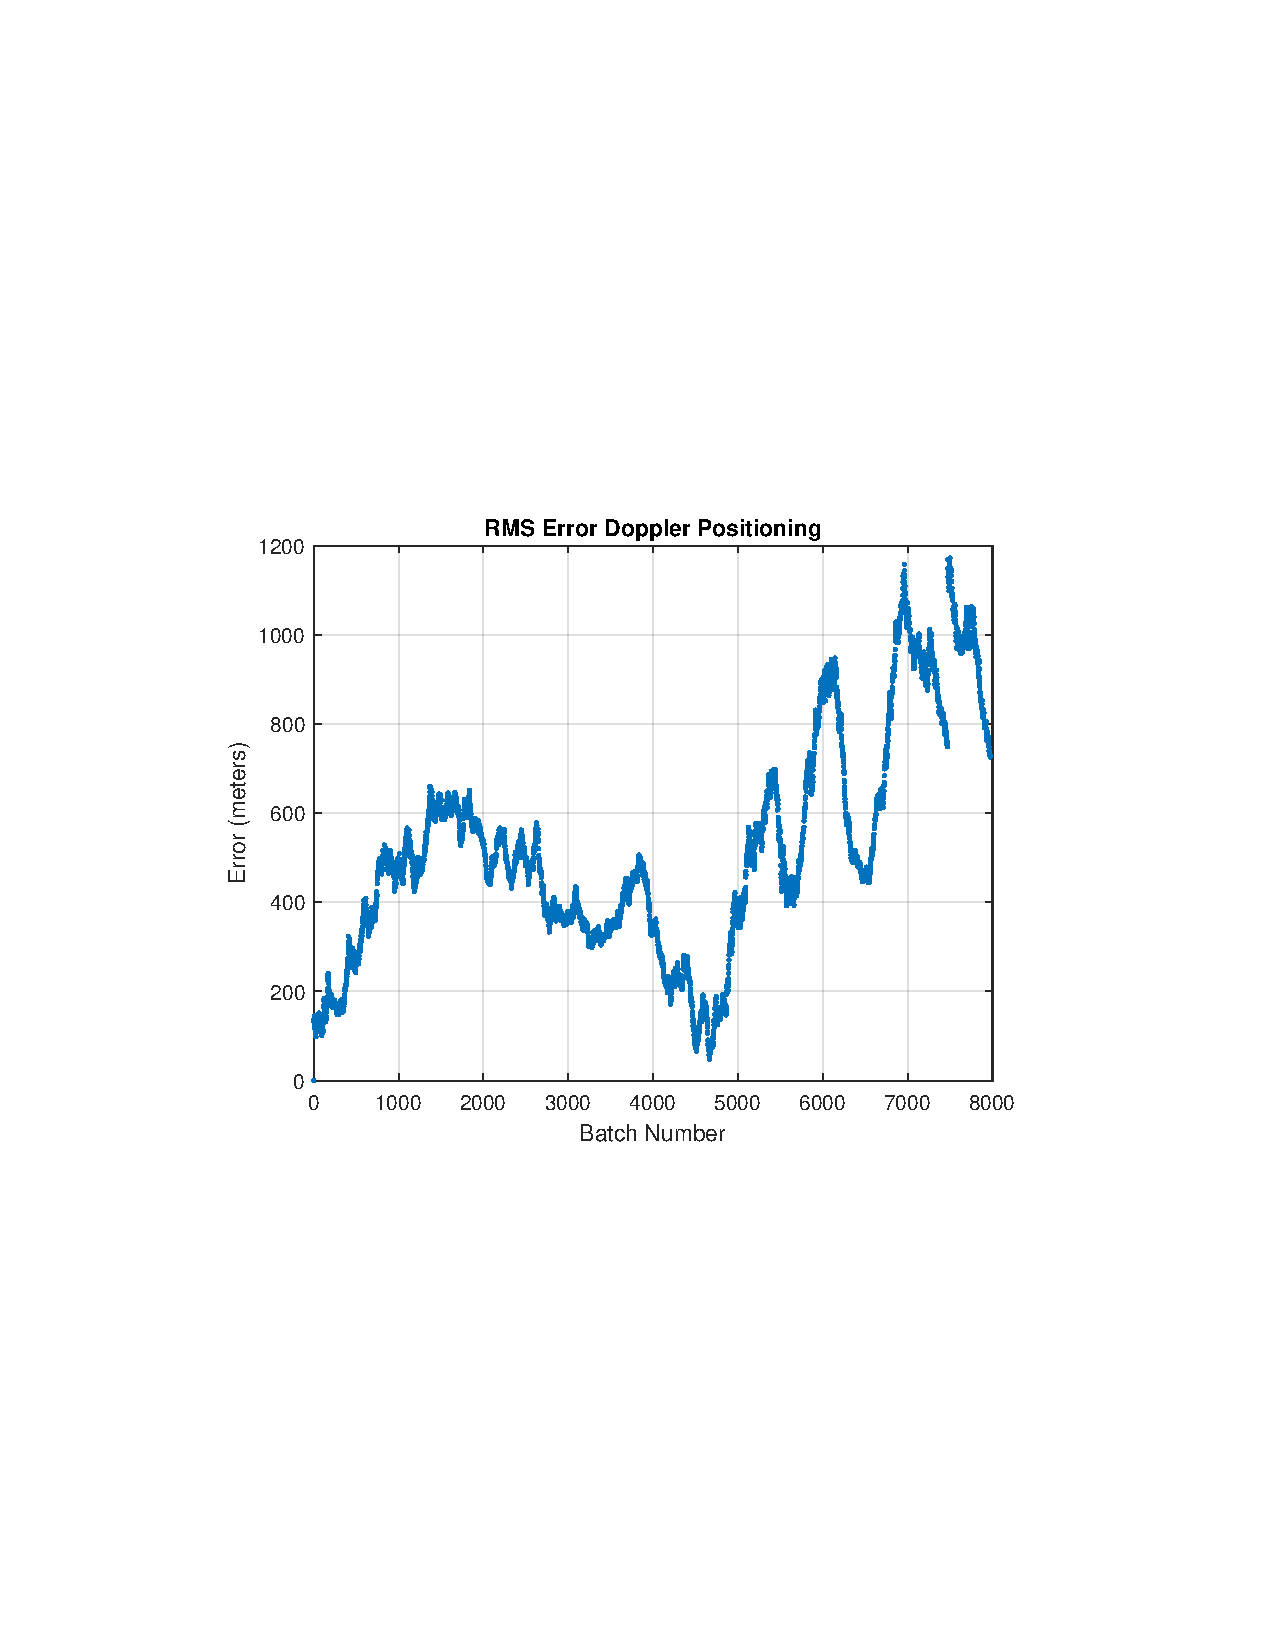
\includegraphics[trim=1.2in 3.3in 1.75in 3.3in,clip,width=5in]{Iridium RMSE plot Doppler Cleanest file.pdf}
    \caption{RMS Error of Batched Doppler Estimates}
    \label{fig:RMSErrorBatchDoppler}
\end{figure}

Figure \ref{fig:PDOPBatchDoppler} shows the PDOP from the batched Doppler measurements. This helps add reasoning to the poor positioning results of the batched doppler positioning. With values ranging from 29 to 52, the PDOP is significantly larger than what would be expected from GPS to give a good positioning solution. 

\begin{figure}[h!]
    \centering
    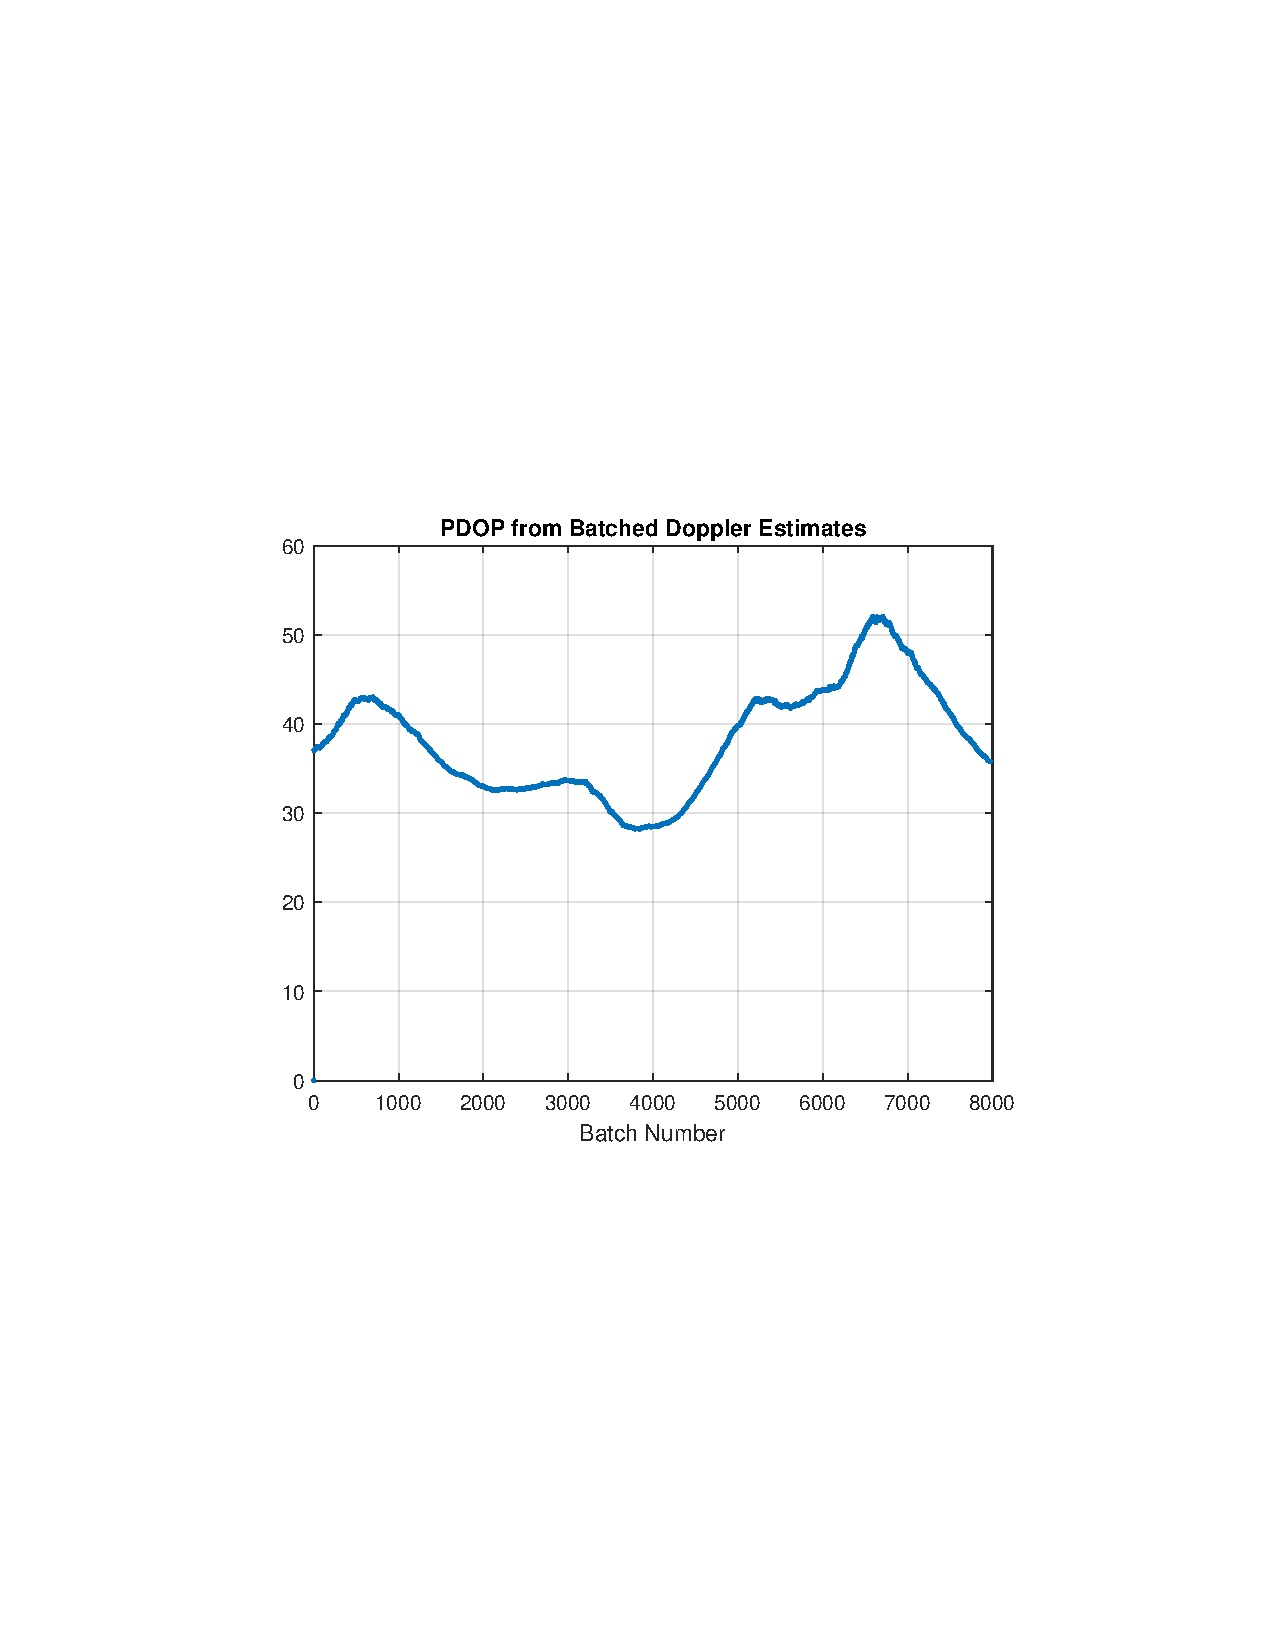
\includegraphics[trim=1.2in 3.3in 1.75in 3.3in,clip,width=5in]{Irid_Clean_15min_doppler_PDOP.pdf}
    \caption{PDOP of Batched Doppler Estimates}
    \label{fig:PDOPBatchDoppler}
\end{figure}

\pagebreak

\subsection{Pseudorange Based Positioning}
The pseudorange based positioning in Section \ref{sec:PseudorangePosTechnique} shows better performance. Figure \ref{fig:CleanPseudo15minIridPosit} shows a geographical plot of the estimated receiver position. 
\begin{figure}[h!]
    \centering
    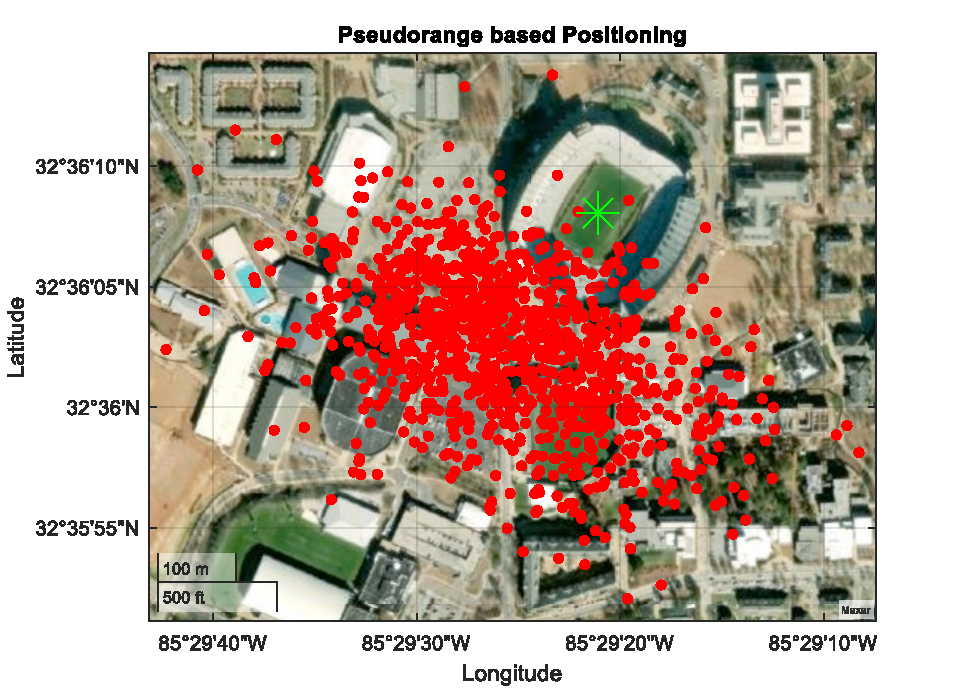
\includegraphics[width=5in]
    {15min_irid_clean_pseudorangebased.pdf}
    \caption{Position Estimate from Pseudoranges}
    \label{fig:CleanPseudo15minIridPosit}
\end{figure}

Figure \ref{fig:CleanPseudo15minIridRSME} shows the root mean square error from truth of the estimated position. The positioning results from this are significantly better than the results from the Doppler positioning. In this technique, measurements are used from multiple satellites at different time points. A positioning solution is only calculated when there are a sufficient number of satellites with unique measurements in view. In most GPS instances, the pseudorange positioning error is 10-15 meters \cite{misraGlobalPositioningSystem2012}. In this instance, the positioning is not as accurate. This could be due to the lower sampling frequency used for this simulation. The resolution of the pseudorange measurements is lowered due to the lower sampling frequency. If the sampling frequency was higher, the change in bit location could be more precisely detected. 
\begin{figure}[h!]
    \centering
    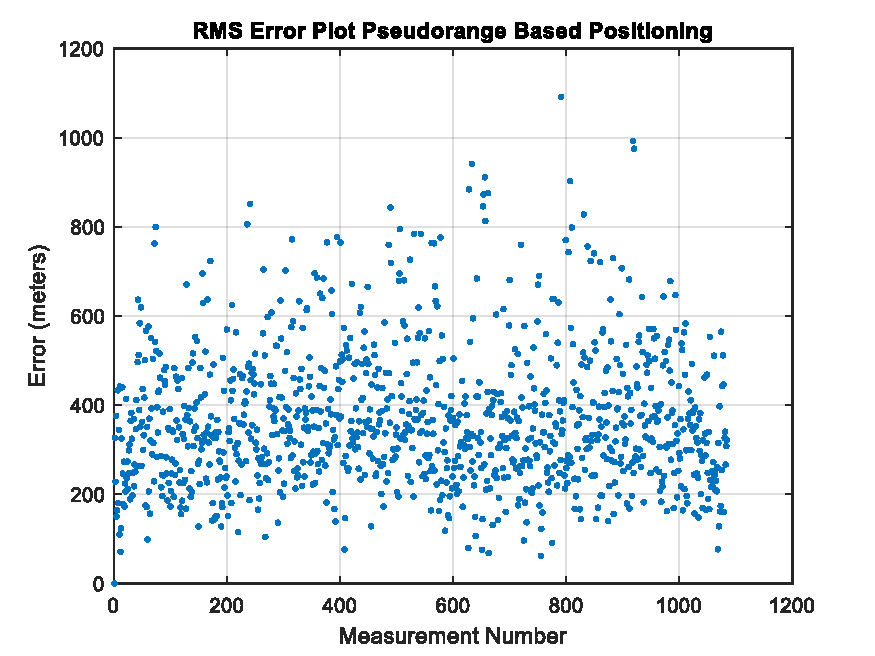
\includegraphics[width=5in]
    {15min_irid_clean_pseudo_rmse.pdf}
    \caption{RMS Error from Pseudoranges}
    \label{fig:CleanPseudo15minIridRSME}
\end{figure}

Figure \ref{fig:CleanPseudo15minIridPositPDOP} shows the PDOP. The PDOP for this simulation is also significantly better than that of the Doppler positioning PDOP and stays around a typical value that would be seen in GPS pseudorange positioning techniques.   
\begin{figure}[h!]
    \centering
    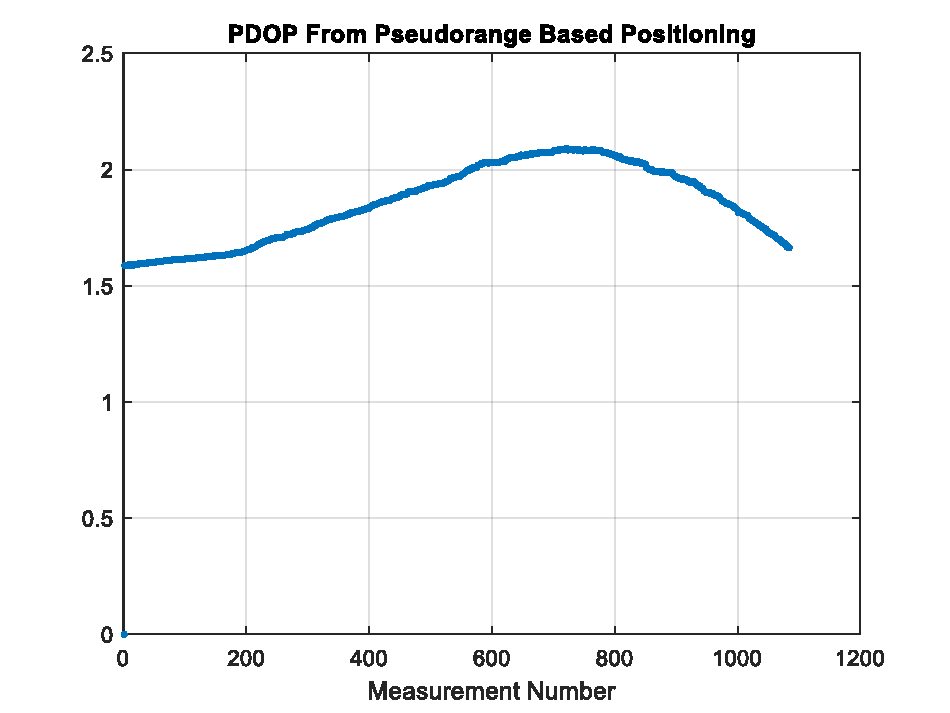
\includegraphics[width=5in]
    {15min_irid_clean_pseudorange_pdop.pdf}
    \caption{PDOP from Pseudoranges}
    \label{fig:CleanPseudo15minIridPositPDOP}
\end{figure}

\section{Static Clean Data Played Through USRP}
For this simulation, everything from the previous simulation remained the same. The signal was passed through a USRP before being processed by the receiver, which was the only difference between the two tests. The USRP used was the B200 mini from Ettus Research. The USRP added thermal background noise, transmitter and receiver clock error, and other unmodeled affects. These errors were expected to contribute to poor positioning results as the errors cannot all be estimated with the algorithms used in this thesis. If the transmitter clock error was known, the receiver clock error could be estimated and vice versa. The algorithm cannot estimate both errors simultaniously. In order to gain a positioning solution, satellite navigation data was filtered to remove outliers in satellite positions and velocities. In this simulation, 9,435 bursts were decoded and 506 bursts were not decoded properly resulting in 94.91 percent decoded. The quadrature bit error rate is 98.0448 percent, and the in-phase bit error rate is 97.8867 percent.

\subsection{Doppler Positioning}
The Doppler positioning geographical plot is shown in Figure \ref{fig:USRPDoppler15minIridPosit}. Initially the positioning results are not terrible, however at batch number 175, the solution begins to grow unbounded. Once the initial guess goes off track, the algorithm cannot correct for the large offset. The estimated position grows due to errors in the decoded satellite navigation message. Even after the error detection the solution grows unbounded. Since each next position estimate is initialized with the previous estimate,the position estimate will become increasingly worse. After batch number 275 the solution grows to infinity and the rest of the estimates cannot be computed. 

\begin{figure}[h!]
    \centering
    \includegraphics[trim=1.2in 3.3in 1.75in 3.3in,clip,width=5in]
    {Irid_15min_USRP_Dopplerposit.pdf}
    \caption{USRP Doppler Positioning Estimate}
    \label{fig:USRPDoppler15minIridPosit}
\end{figure}

Figure \ref{fig:USRPDoppler15minIridRMSE} shows the error seen in Figure \ref{fig:USRPDoppler15minIridPosit}. Again, it can be seen that the error grows around batch number 175 and then returns closer to truth after batch number 250. It would have been expected to see 8000 batched positioning solutions, however less than 300 were computed. This because once the diverts from a value near truth, the solution grows unbounded towards infinity. 

\begin{figure}[h!]
    \centering
    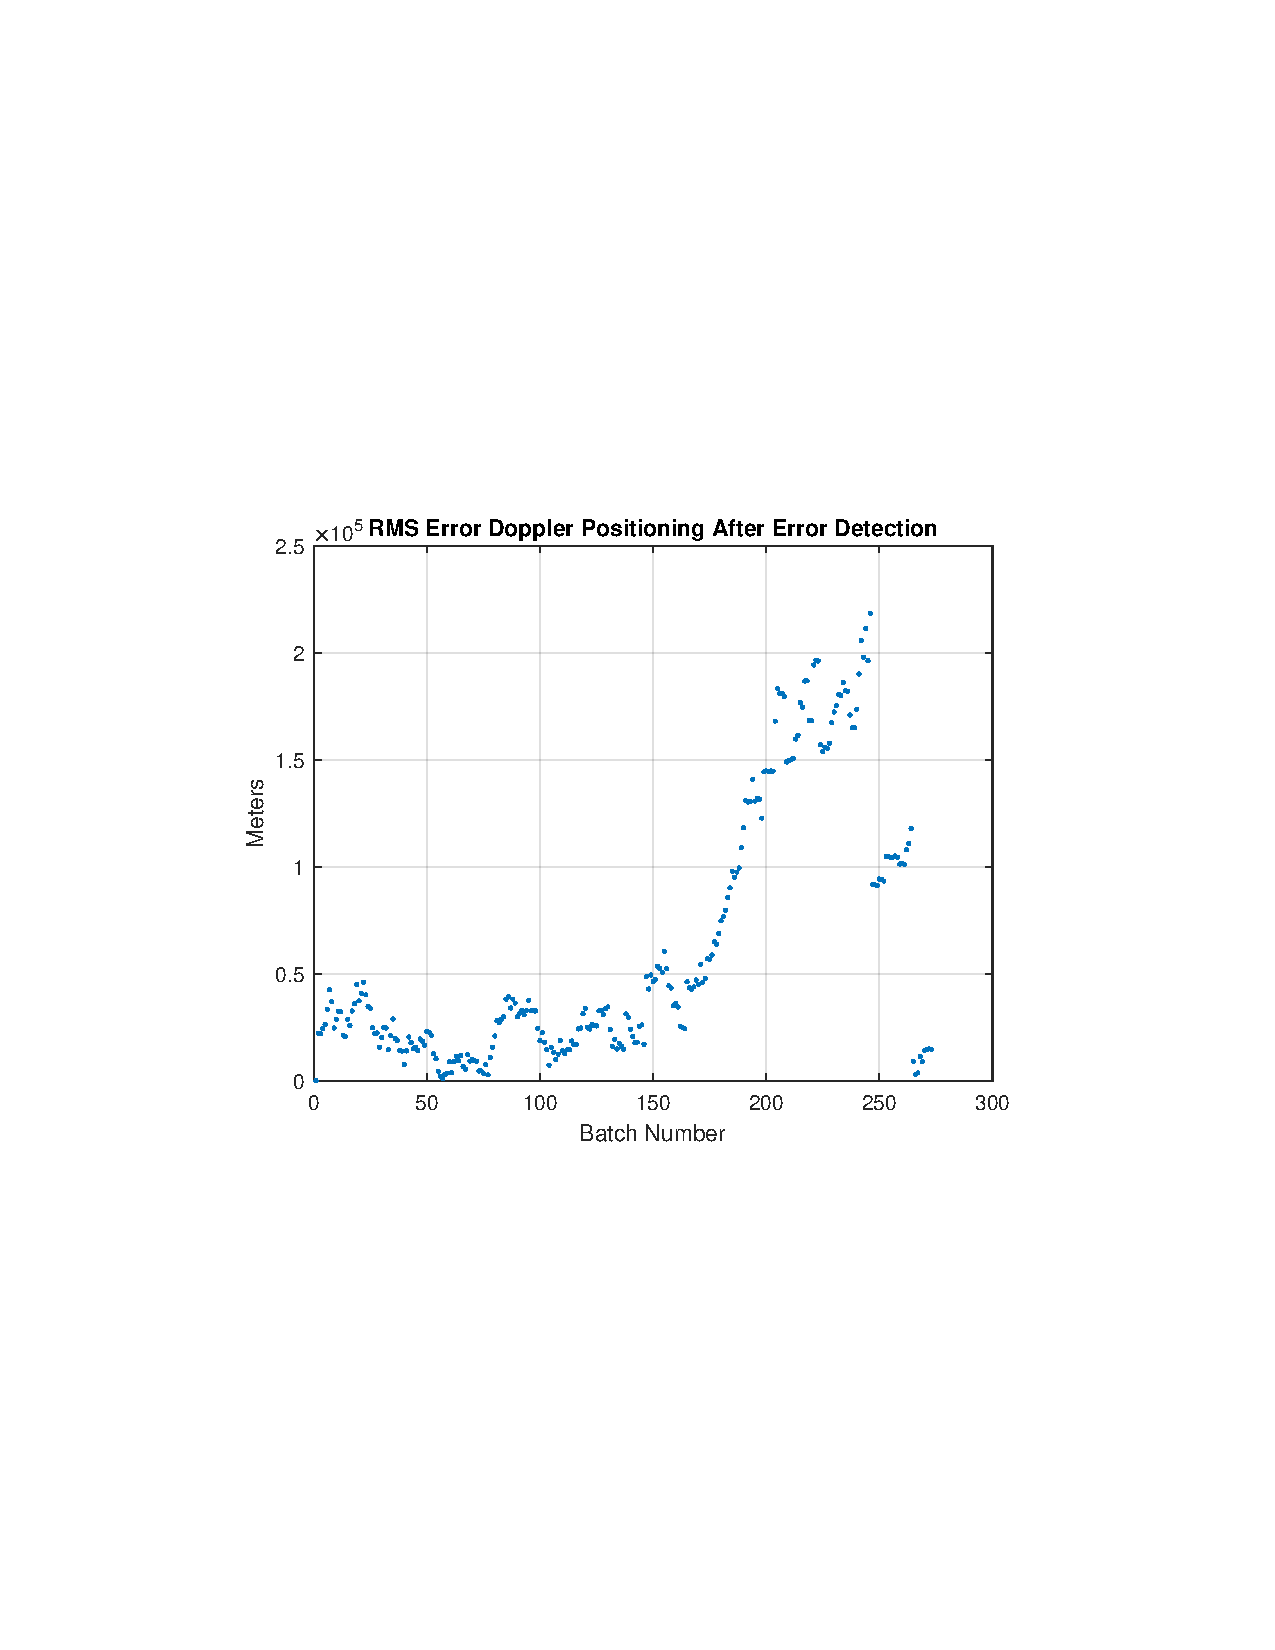
\includegraphics[trim=1.2in 3.3in 1.75in 3.3in,clip,width=5in]
    {Irid_15min_USRP_DopplerRMSE.pdf}
    \caption{RMS Error of Doppler Positioning Estimate}
    \label{fig:USRPDoppler15minIridRMSE}
\end{figure}

Figure \ref{fig:USRPDoppler15minIridPDOP} shows at the begining of the simulation, the PDOP is poor. The PDOP remains around 3000 until near the end where it begins to decrease, however the measurement errors cause the estimate to grow unbounded and no more estimates to be calculated. 
\begin{figure}[h!]
    \centering
    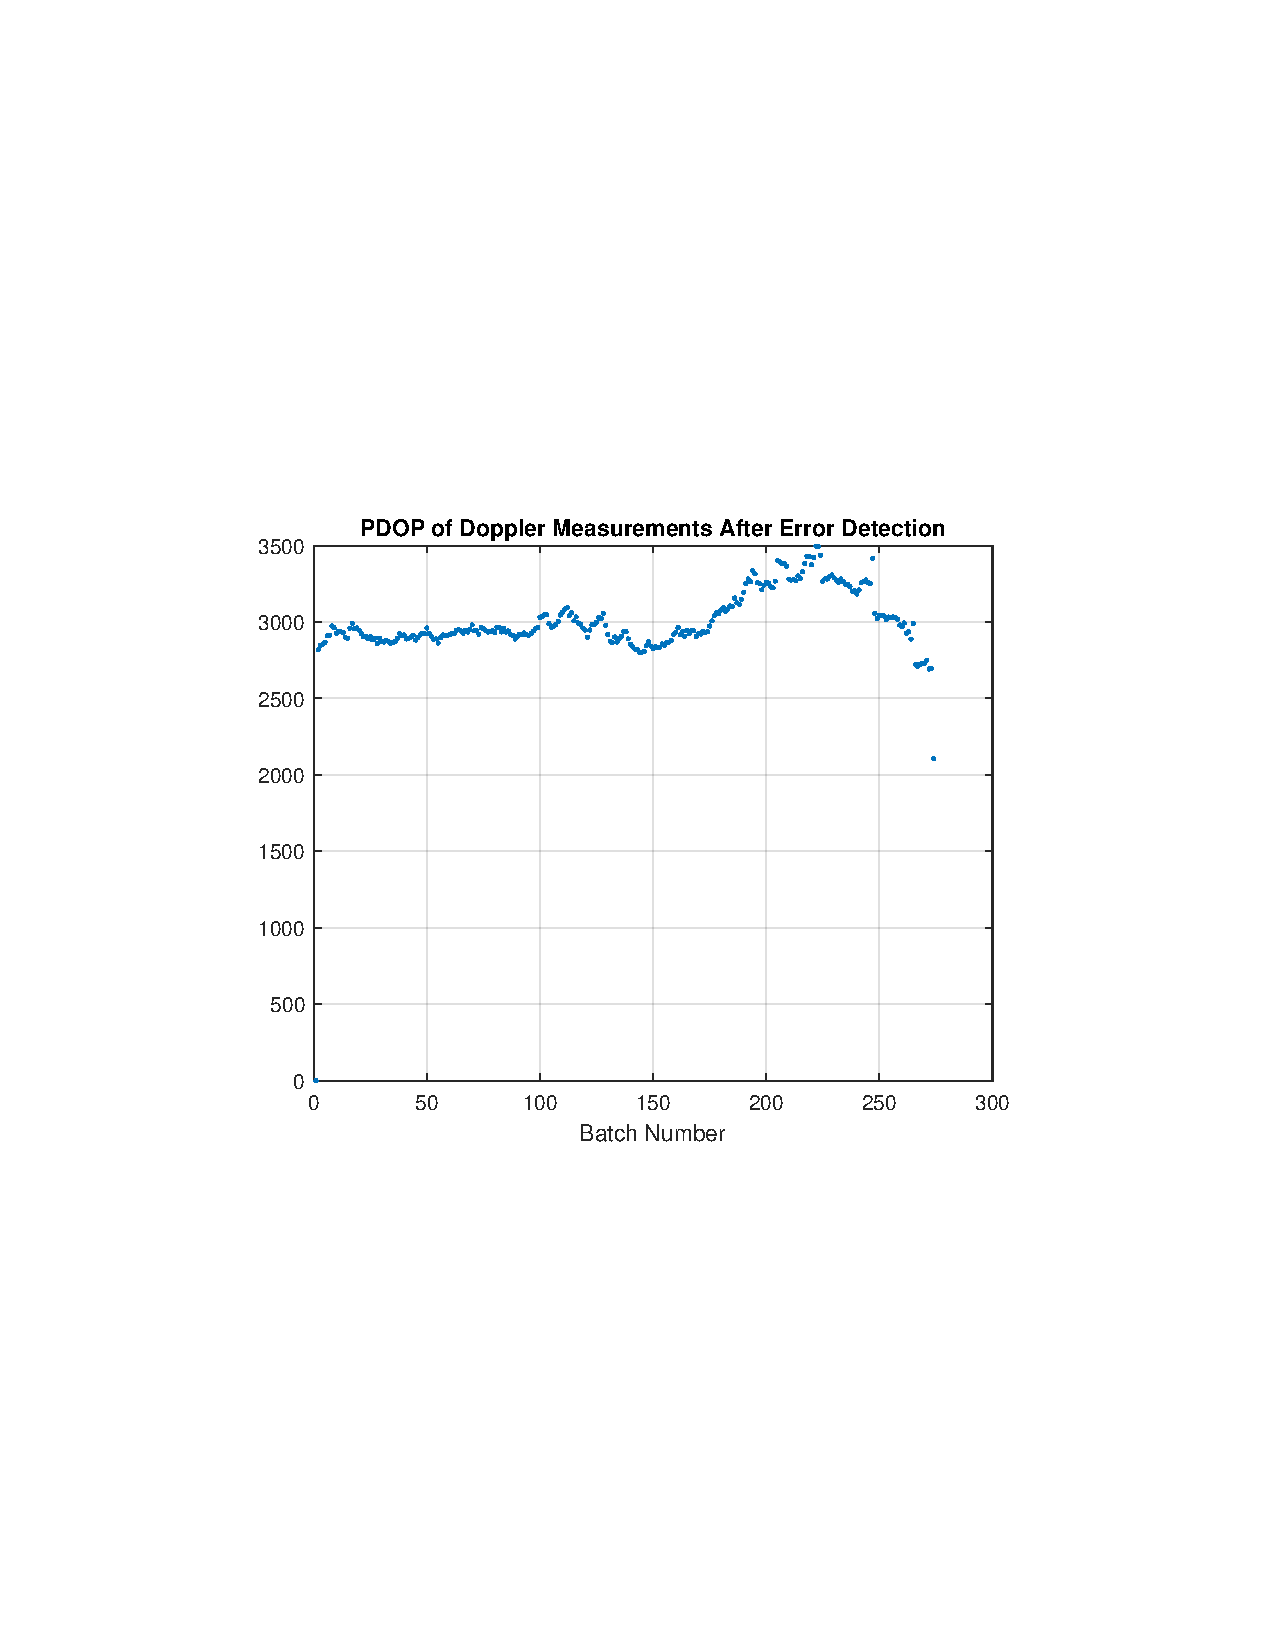
\includegraphics[trim=1.2in 3.3in 1.75in 3.3in,clip,width=5in]
    {Irid_15min_USRP_DopplerPDOP.pdf}
    \caption{PDOP from Doppler Positioning Estimate}
    \label{fig:USRPDoppler15minIridPDOP}
\end{figure}

\pagebreak
\subsection{Pseudorange Based Positioning}
Figure \ref{fig:USRPpseudo15minIridPosit} gives the geo plot of the pseudorange based positioning estimates. The pseudorange based positioning is better, but is still poor when compared to the case with no noise. 
\begin{figure}[h!]
    \centering
    \includegraphics[trim=1.2in 3.3in 1.6in 3.3in,clip,width=5in]
    {Irid_15min_USRP_Pseudoposit.pdf}
    \caption{USRP Pseurorange Positioning Estimate}
    \label{fig:USRPpseudo15minIridPosit}
\end{figure}
The position can be seen drifting across the geo plot. This may be caused by the clock error in the USRP. Figure \ref{fig:USRPpseudo15minIridRMSE} shows that the majority of the position estimates remain low, however there are still some outlier position estimates. Other possible errors could be caused by bit errors caused by the USRP. This would cause the change in bit location to have error contributing to noisy pseudorange measurements. 
\begin{figure}[h!]
    \centering
    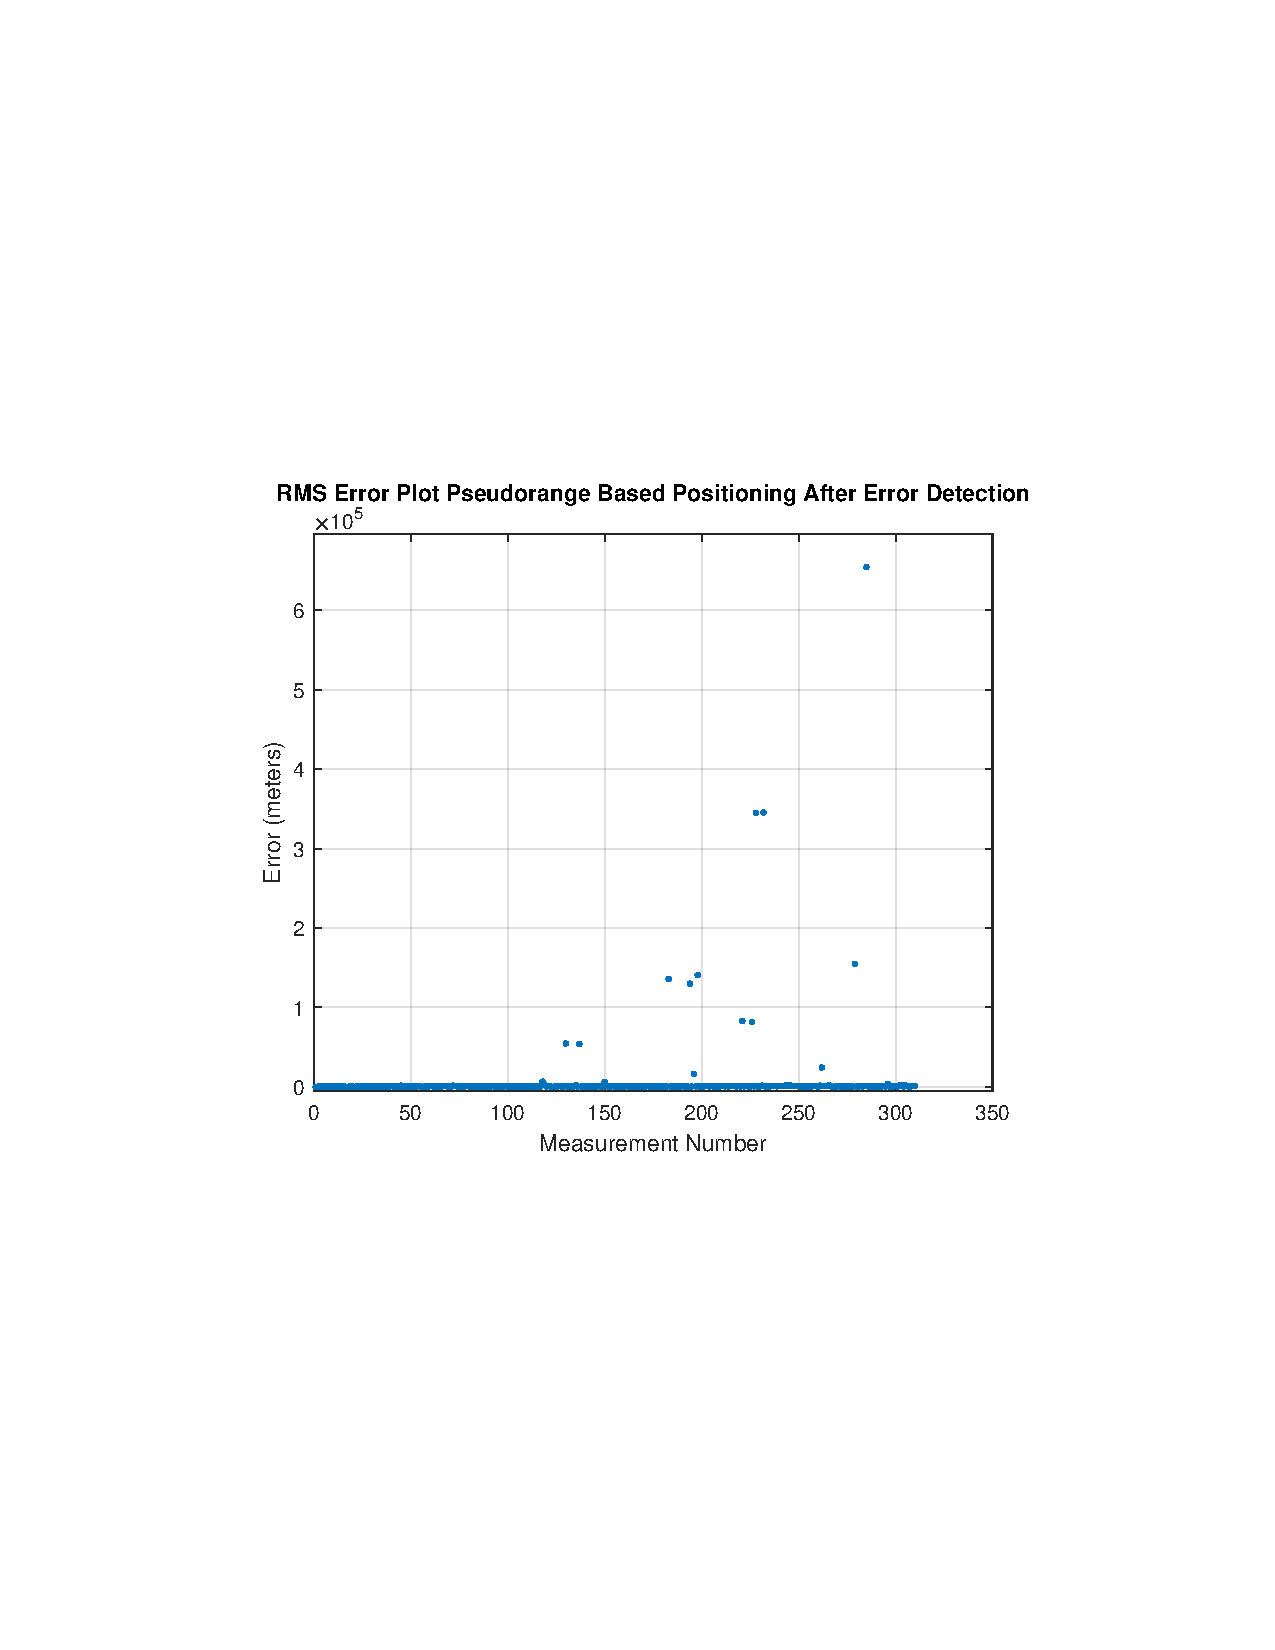
\includegraphics[trim=1.2in 3.3in 1.6in 2.9in,clip,width=5in]
    {Irid_15min_USRP_PseudoRMS.pdf}
    \caption{RMS Error USRP Pseurorange Positioning Estimate}
    \label{fig:USRPpseudo15minIridRMSE}
\end{figure}

Figure \ref{fig:USRPpseudo15minIridPositpdop} shows the PDOP from the pseudorange based positioning estimate. The PDOP is significantly better than the PDOP from the Doppler based positioning. However instead of being a smooth curve as expected, there are outliers along the curve that match the same position as the larger positioning errors. 
\begin{figure}[h!]
    \centering
    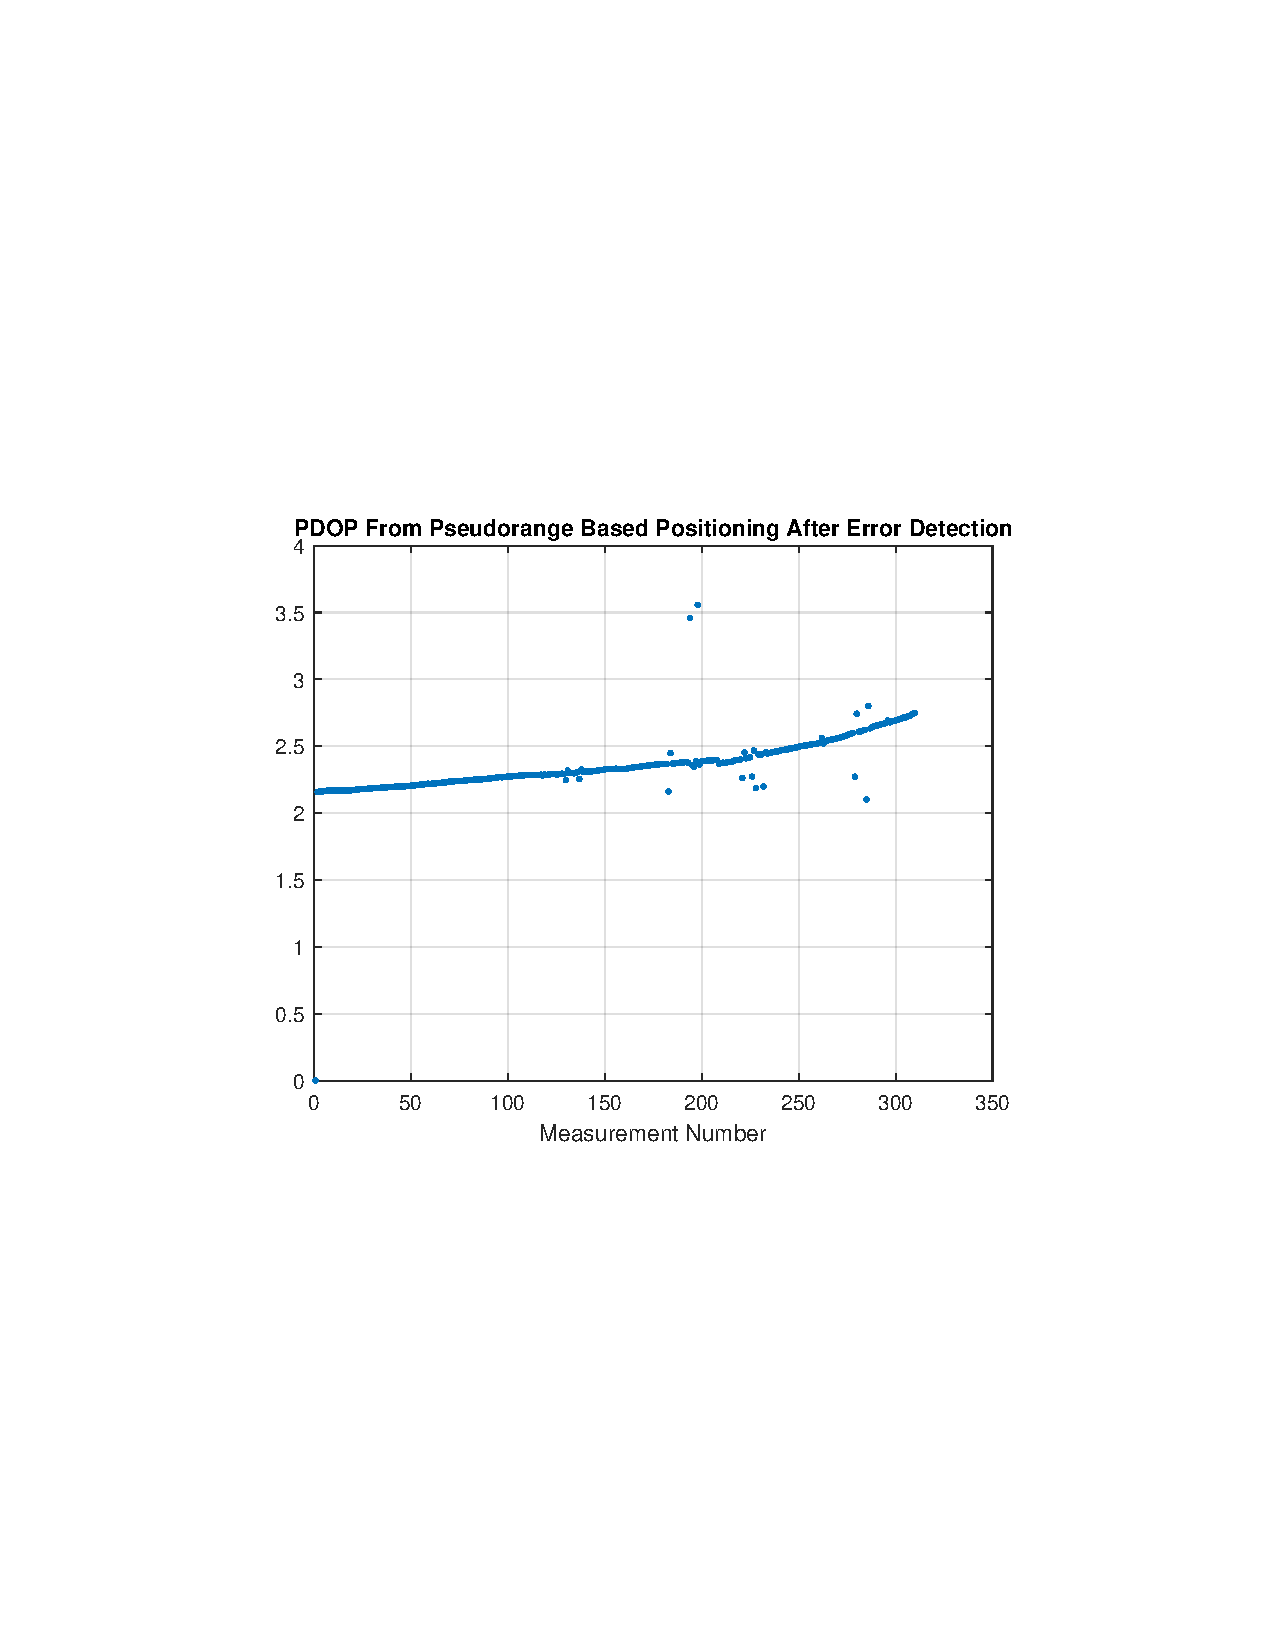
\includegraphics[trim=1.2in 3.3in 1.75in 3.3in,clip,width=5in]
    {Irid_15min_USRP_PseudoPDOP.pdf}
    \caption{USRP Pseurorange Positioning Estimate PDOP}
    \label{fig:USRPpseudo15minIridPositpdop}
\end{figure}

\section{Static Noisy Data}
In this section, a simulated signal with signal noise and measurement noise is generated. The user clock was modeled as an OCXO. The satellite clock error is simulated as zero for simplicity. This is because the error caused by the satellite clock would be transmitted and imediately be removed from the measurement. IridiumNext was the constellation used. The simulation length was 15 minutes, and the truth receiver location was [32.602236,-85.489192,201]. The carrier to noise ratio for the signal is set to 65. The quadrature bit rate error is 98.5423 percent and the in-phase bit rate error is 99.1743 percent. 

\subsection{Doppler Positioning}
The Doppler positioning of this data set is shown in Figure \ref{fig:DirtyDoppler15minIridPosit}. This solution is better than the estimates provided from the USRP data set. The batch size used for this position estimate is 2000 measurements. 
\begin{figure}[h!]
    \centering
    \includegraphics[trim=1.2in 3.3in 1.75in 3.3in,clip,width=5in]
    {Irid_15min_noisy_positdoppler.pdf}
    \caption{Noisy Doppler Positioning Estimate}
    \label{fig:DirtyDoppler15minIridPosit}
\end{figure}

Figure \ref{fig:DirtyDoppler15minIridPositrmse} shows the RMS error from truth. The closest estimate is near 1000 meters with a maximum error around 4250 meters. These errors can be attributed to the error caused by the received Doppler estimates and the clock drift. While the clock drift is estimated by the receiver, batching causes error in this estimate. This is because the clock drift is averaged across all the measurements over time instead of instantaneously. For example, if the batch number is 2000 and the burst time is 0.09s, there are 180 seconds where the drift grows. 

\begin{figure}[h!]
    \centering
    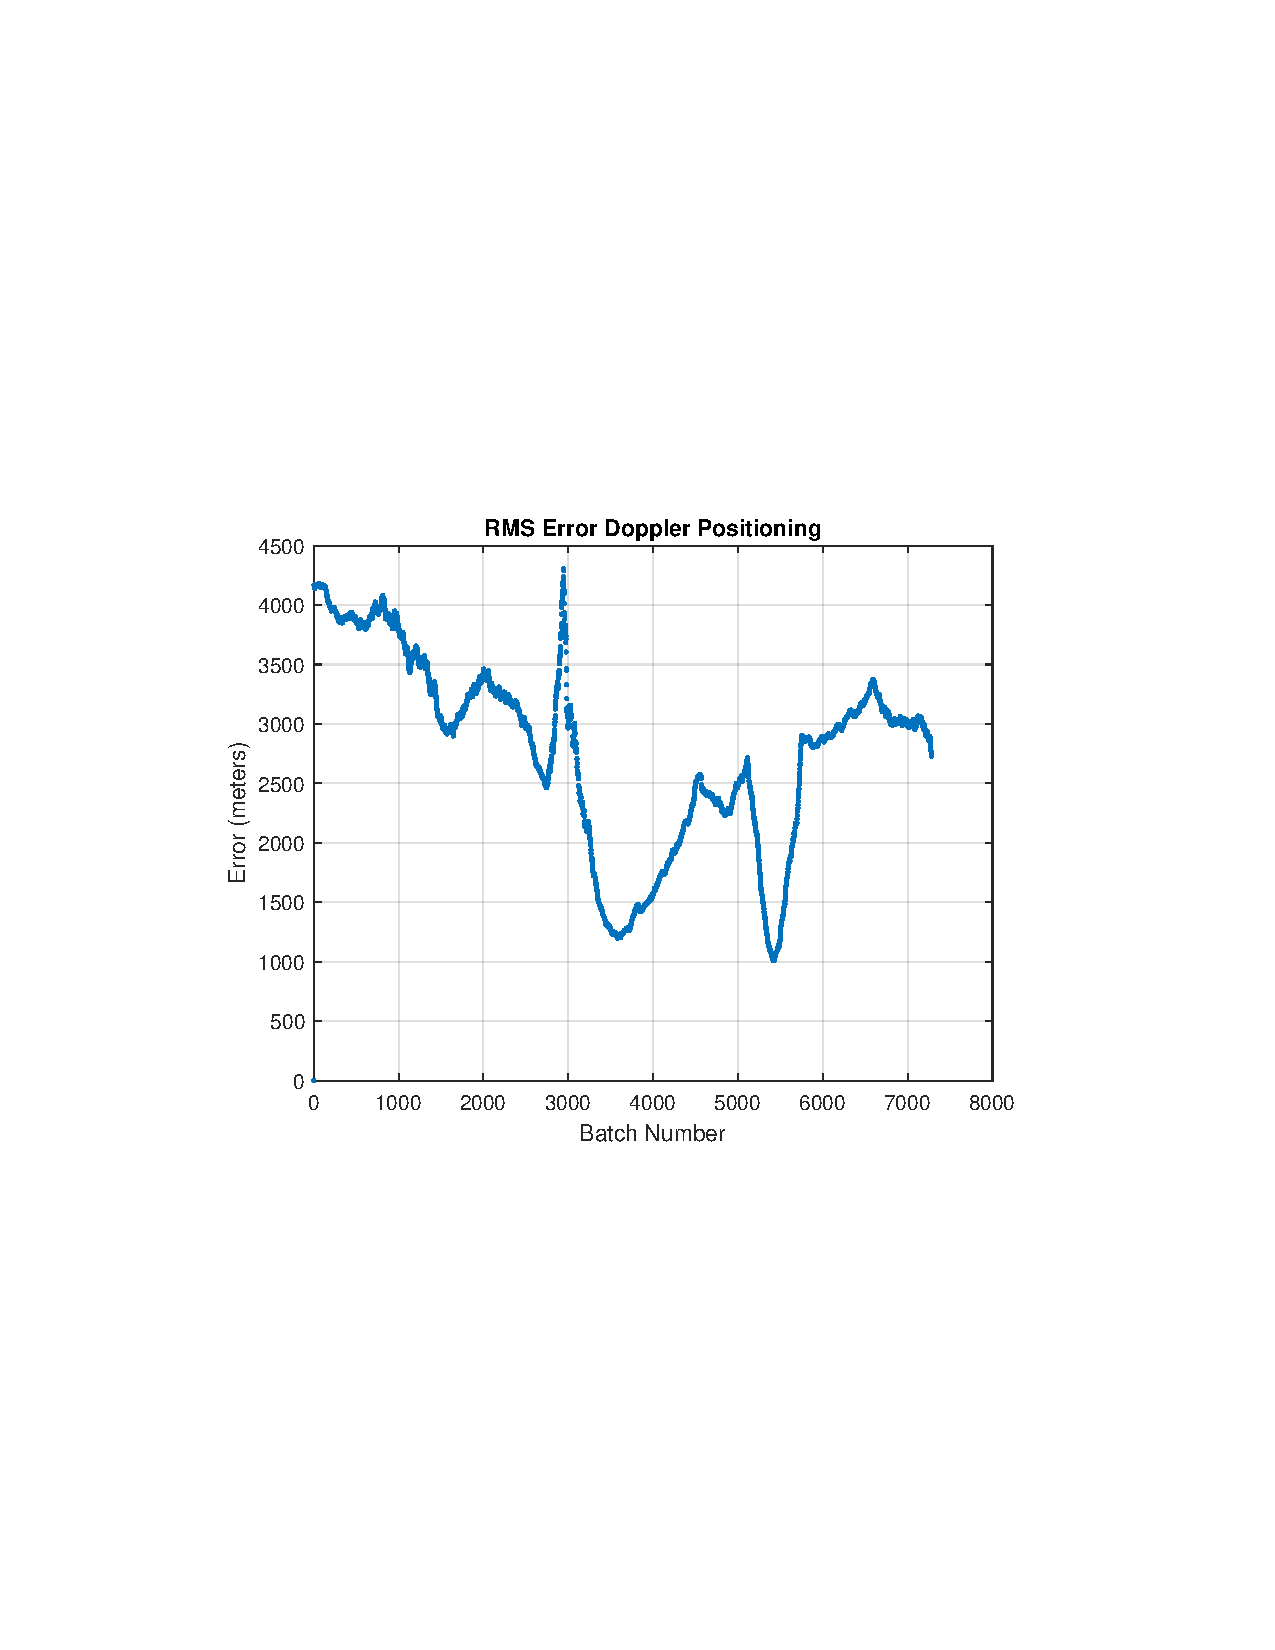
\includegraphics[trim=1.2in 3.3in 1.75in 3.3in,clip,width=5in]
    {Irid_15min_noisy_RMSEdoppler.pdf}
    \caption{RMS Error Noisy Doppler Positioning Estimate}
    \label{fig:DirtyDoppler15minIridPositrmse}
\end{figure}

Figure \ref{fig:DirtyDoppler15minIridPDOP} shows the PDOP across the batches. The spike in error around batch number 3000 could be attributed to the spike in PDOP. At this point, the diversity in satellites is lower and most of the measurements are coming from one satellite instead of multiple. The drop in PDOP is where an additional satellite comes into view and there is more diversity in the satellite measurements. 
\begin{figure}[h!]
    \centering
    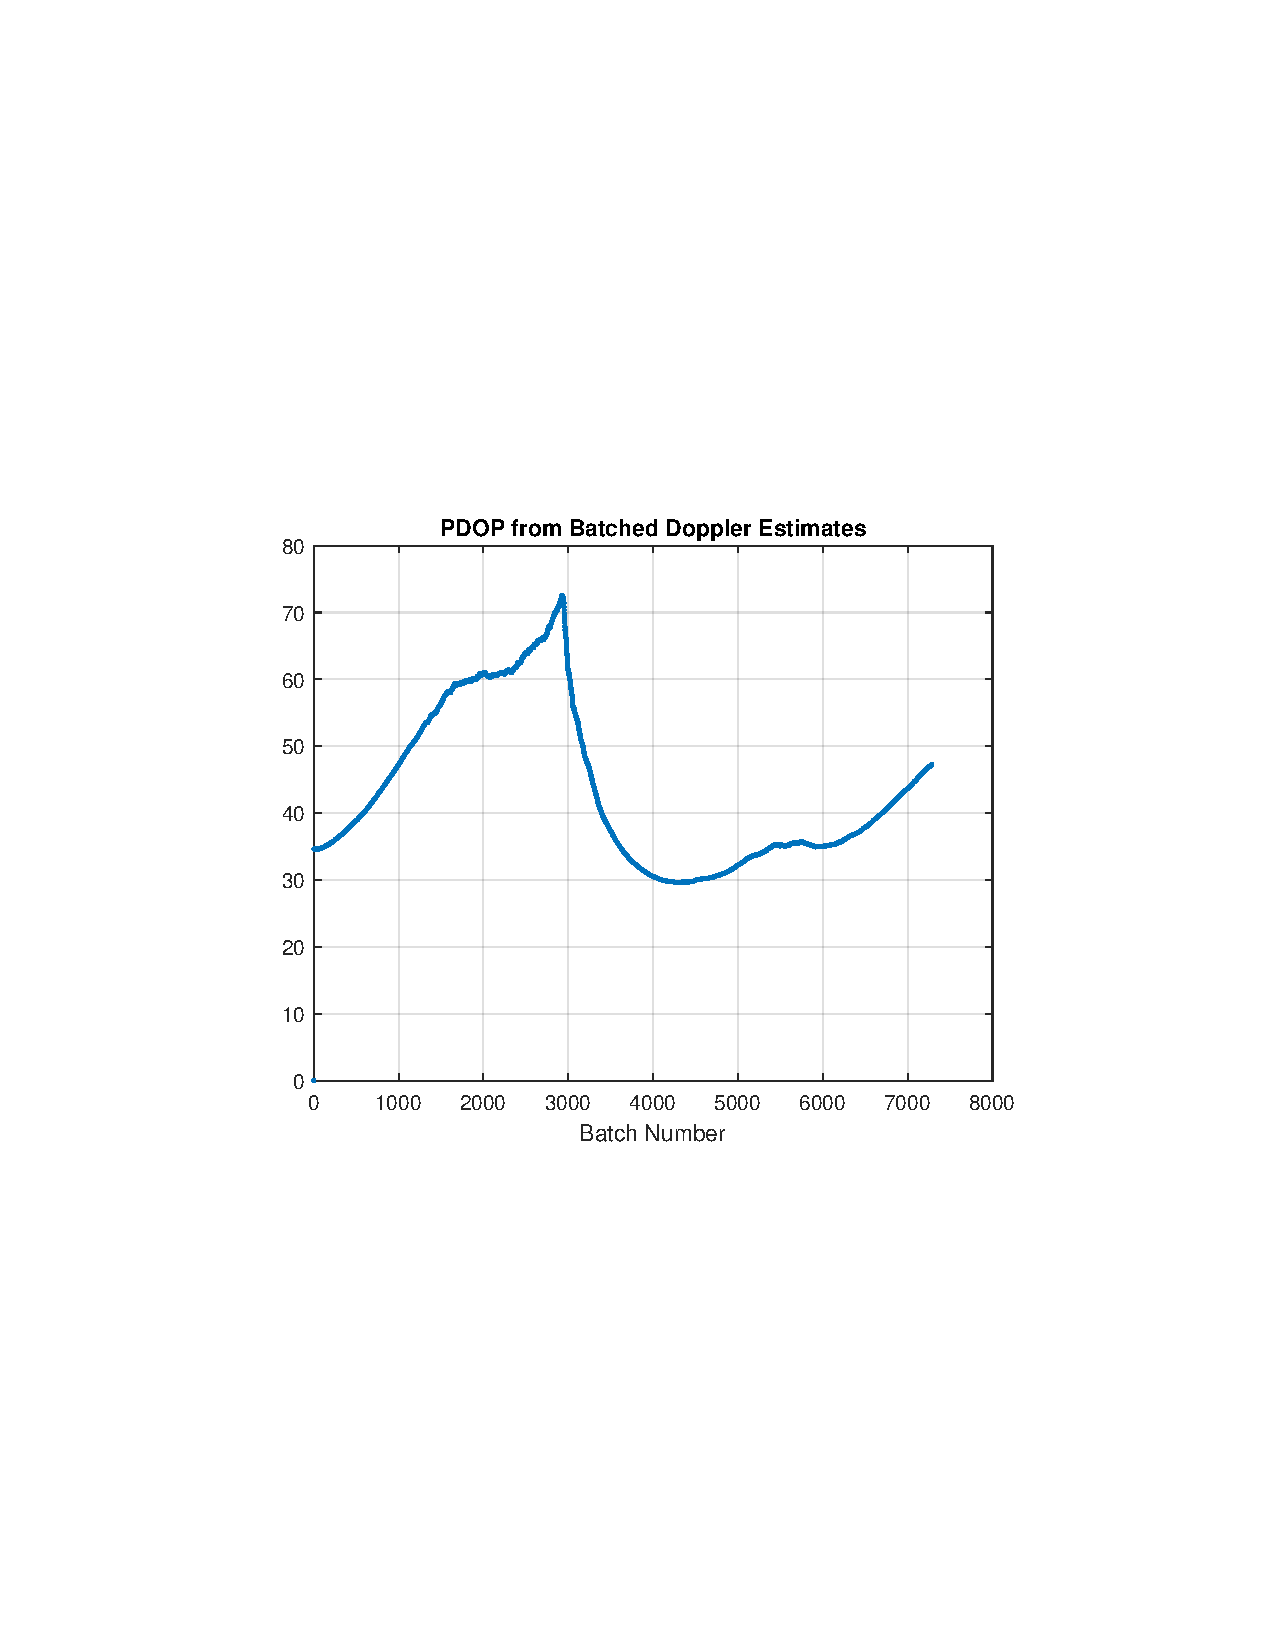
\includegraphics[trim=1.2in 3.3in 1.75in 3.3in,clip,width=5in]
    {Irid_15min_noisy_PDOPdoppler.pdf}
    \caption{Noisy Doppler Positioning PDOP}
    \label{fig:DirtyDoppler15minIridPDOP}
\end{figure}

\pagebreak
\subsection{Pseudorange Based Positioning}
Figure \ref{fig:DirtyPseudorange15minIridPosit} shows the geo plot of the pseudorange based positioning. In this example, the pseudorange has tropospheric error, clock bias, and additional un-modeled effects with a mean of 5 meters. This figure shows receiver estimate when the errors have not been taken out of the measurement. The error is worse than the Doppler based positioning. 
\begin{figure}[h!]
    \centering
    \includegraphics[trim=1.2in 3.3in 1.75in 3.3in,clip,width=5in]
    {Irid_15min_noisy_Positpseudo.pdf}
    \caption{Noisy Pseudorange Positioning Estimate}
    \label{fig:DirtyPseudorange15minIridPosit}
\end{figure}
Figure \ref{fig:DirtyPseudorange15minIridPositrmse} shows the distribution RMS error of the pseudorange based positioning. At its highest, the error is nearly 30 kilometers, where the lowest is within 100 meters. 
\begin{figure}[h!]
    \centering
    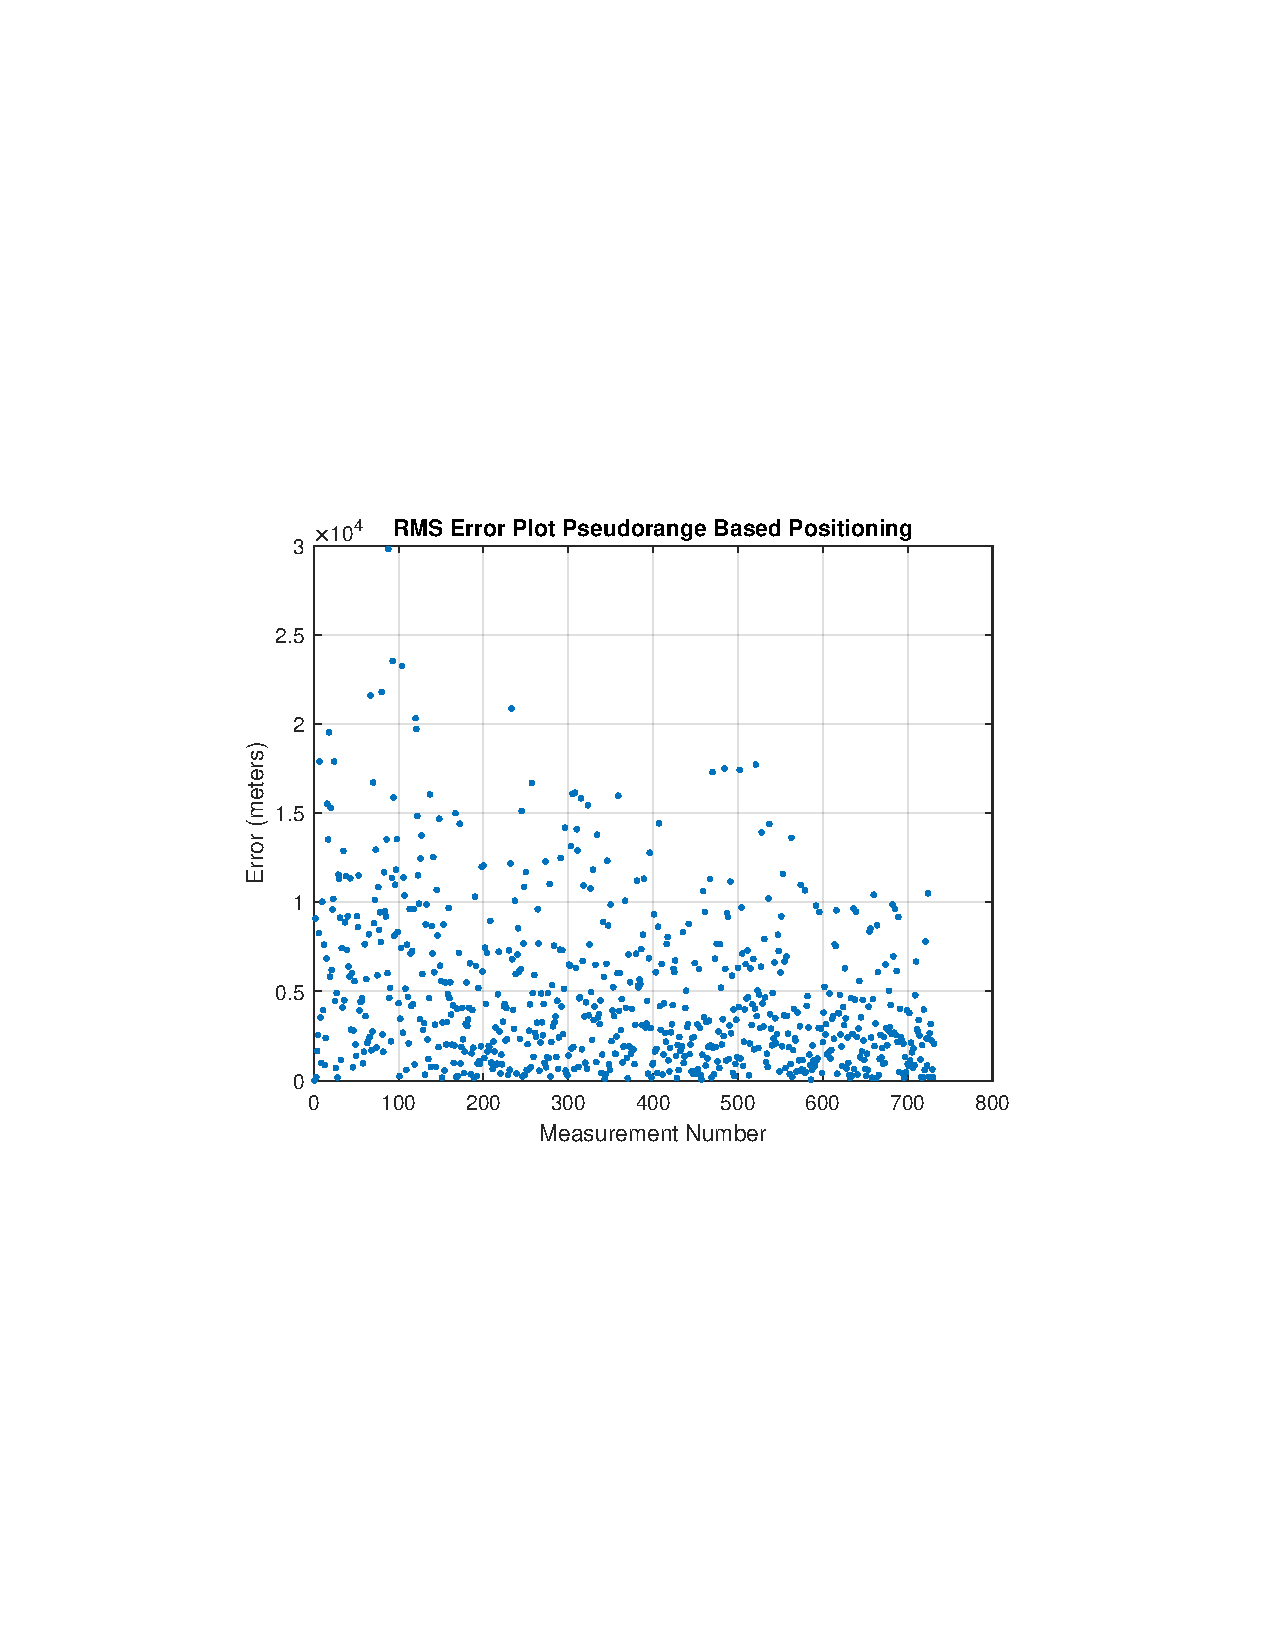
\includegraphics[trim=1.2in 3.3in 1.75in 3.3in,clip,width=5in]
    {Irid_15min_noisy_RMSEpseudo.pdf}
    \caption{RMS Error Noisy Pseudorange Positioning Estimate}
    \label{fig:DirtyPseudorange15minIridPositrmse}
\end{figure}

The PDOP in Figure \ref{fig:PDOPDirtyPseudorange15minIridPosit} is the highest of all the simulations. It starts near 57 and eventually trails off to 22.
\begin{figure}[h!]
    \centering
    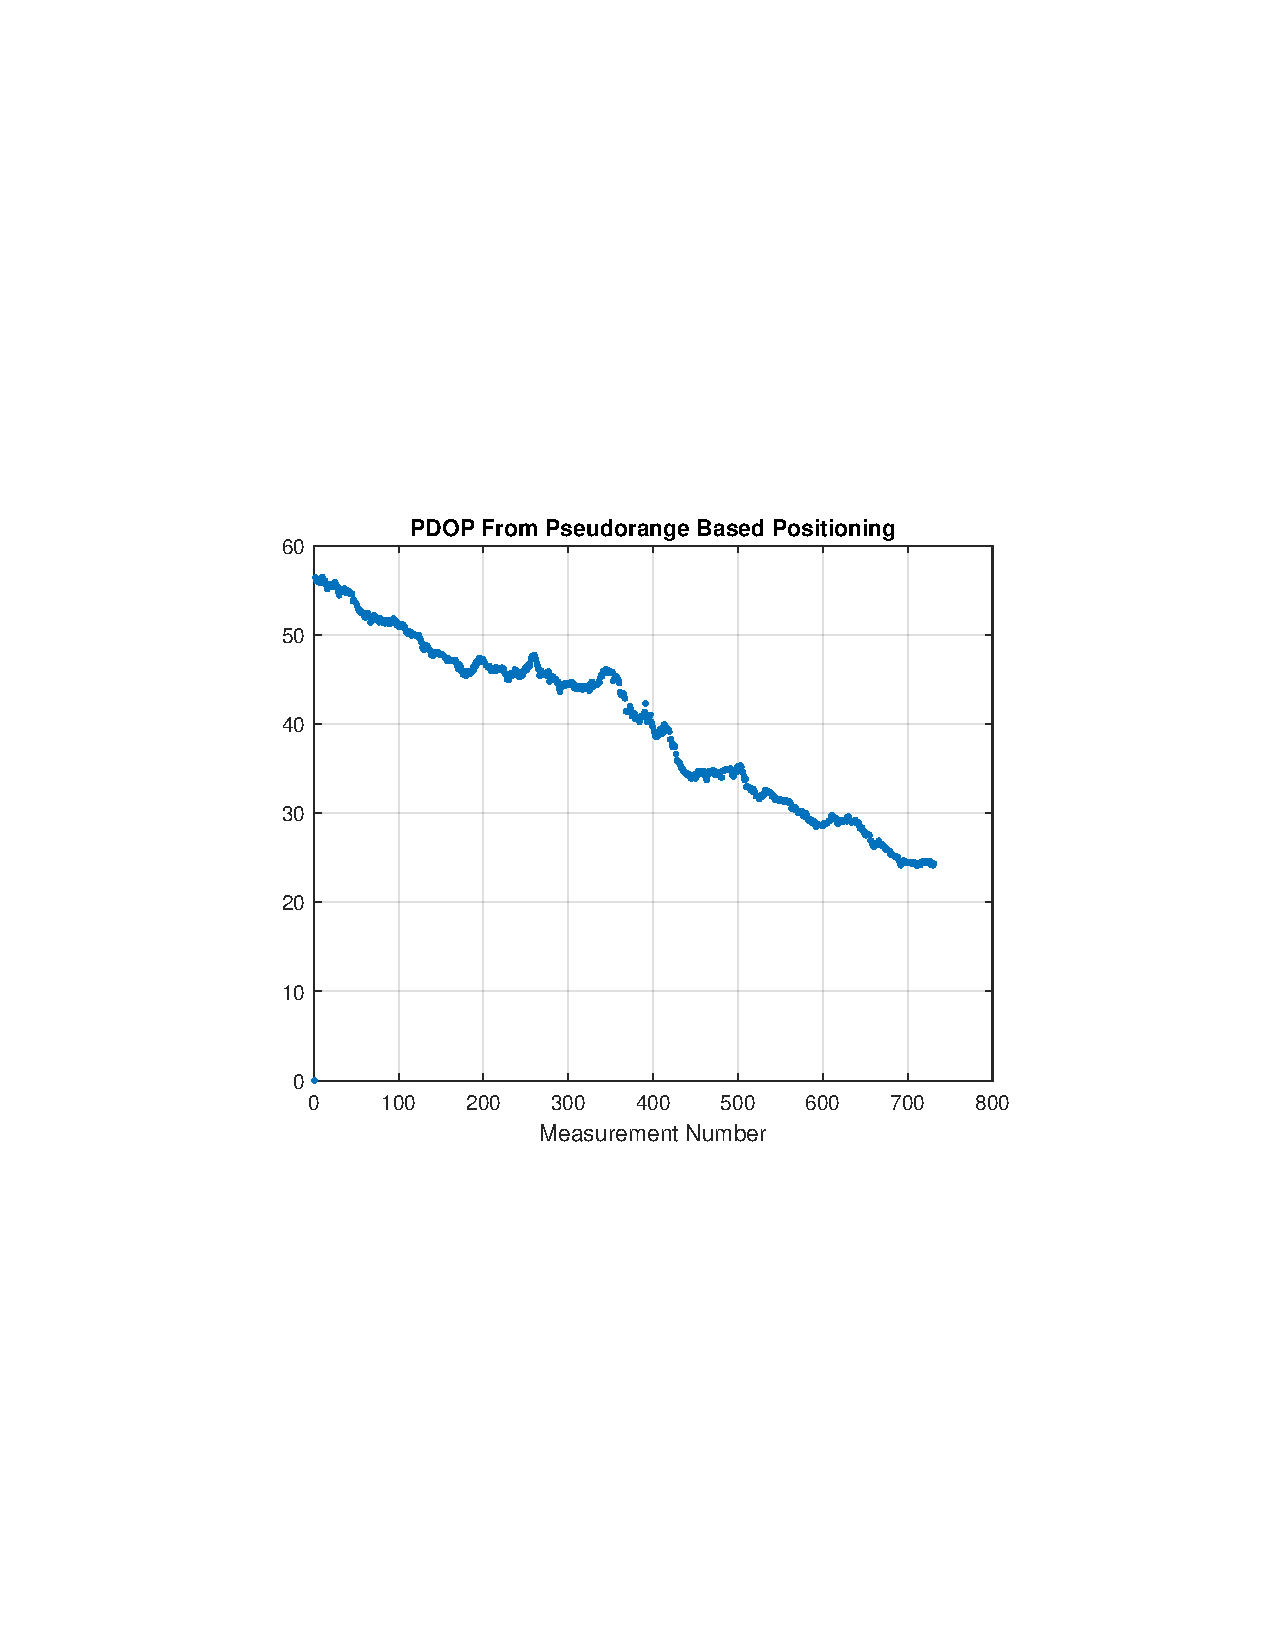
\includegraphics[trim=1.2in 3.3in 1.75in 3.3in,clip,width=5in]
    {Irid_15min_noisy_PDOPpseudo.pdf}
    \caption{PDOP Dirty Pseudorange Positioning Estimate}
    \label{fig:PDOPDirtyPseudorange15minIridPosit}
\end{figure}

\pagebreak
\section{Static Augmented Satellites}
To show the versitility of the simulation tool, a simulation of augmented satellites was performed. In this simulation, the length is 5 minutes. The main satellite constellation is the IridiumNext constellation. All noise terms are turned off. The augmented constellation has 8 orbital planes, 15 satellites per plane, an inclination angle of 45 degrees, and an orbit altitude of 800 kilometers. The receiver is placed at the 50 yard line of Jordan-Hare Stadium in Auburn, Alabama [32.602236,-85.489192,201]. The bit error rate for bith the in-phase and quadrature are 99.9624 percent. Figure \ref{fig:AugmentGlobe} shows the orbit paths of the IridiumNext constellation augmented with additional satellites. 

\begin{figure}[h!]
    \centering
    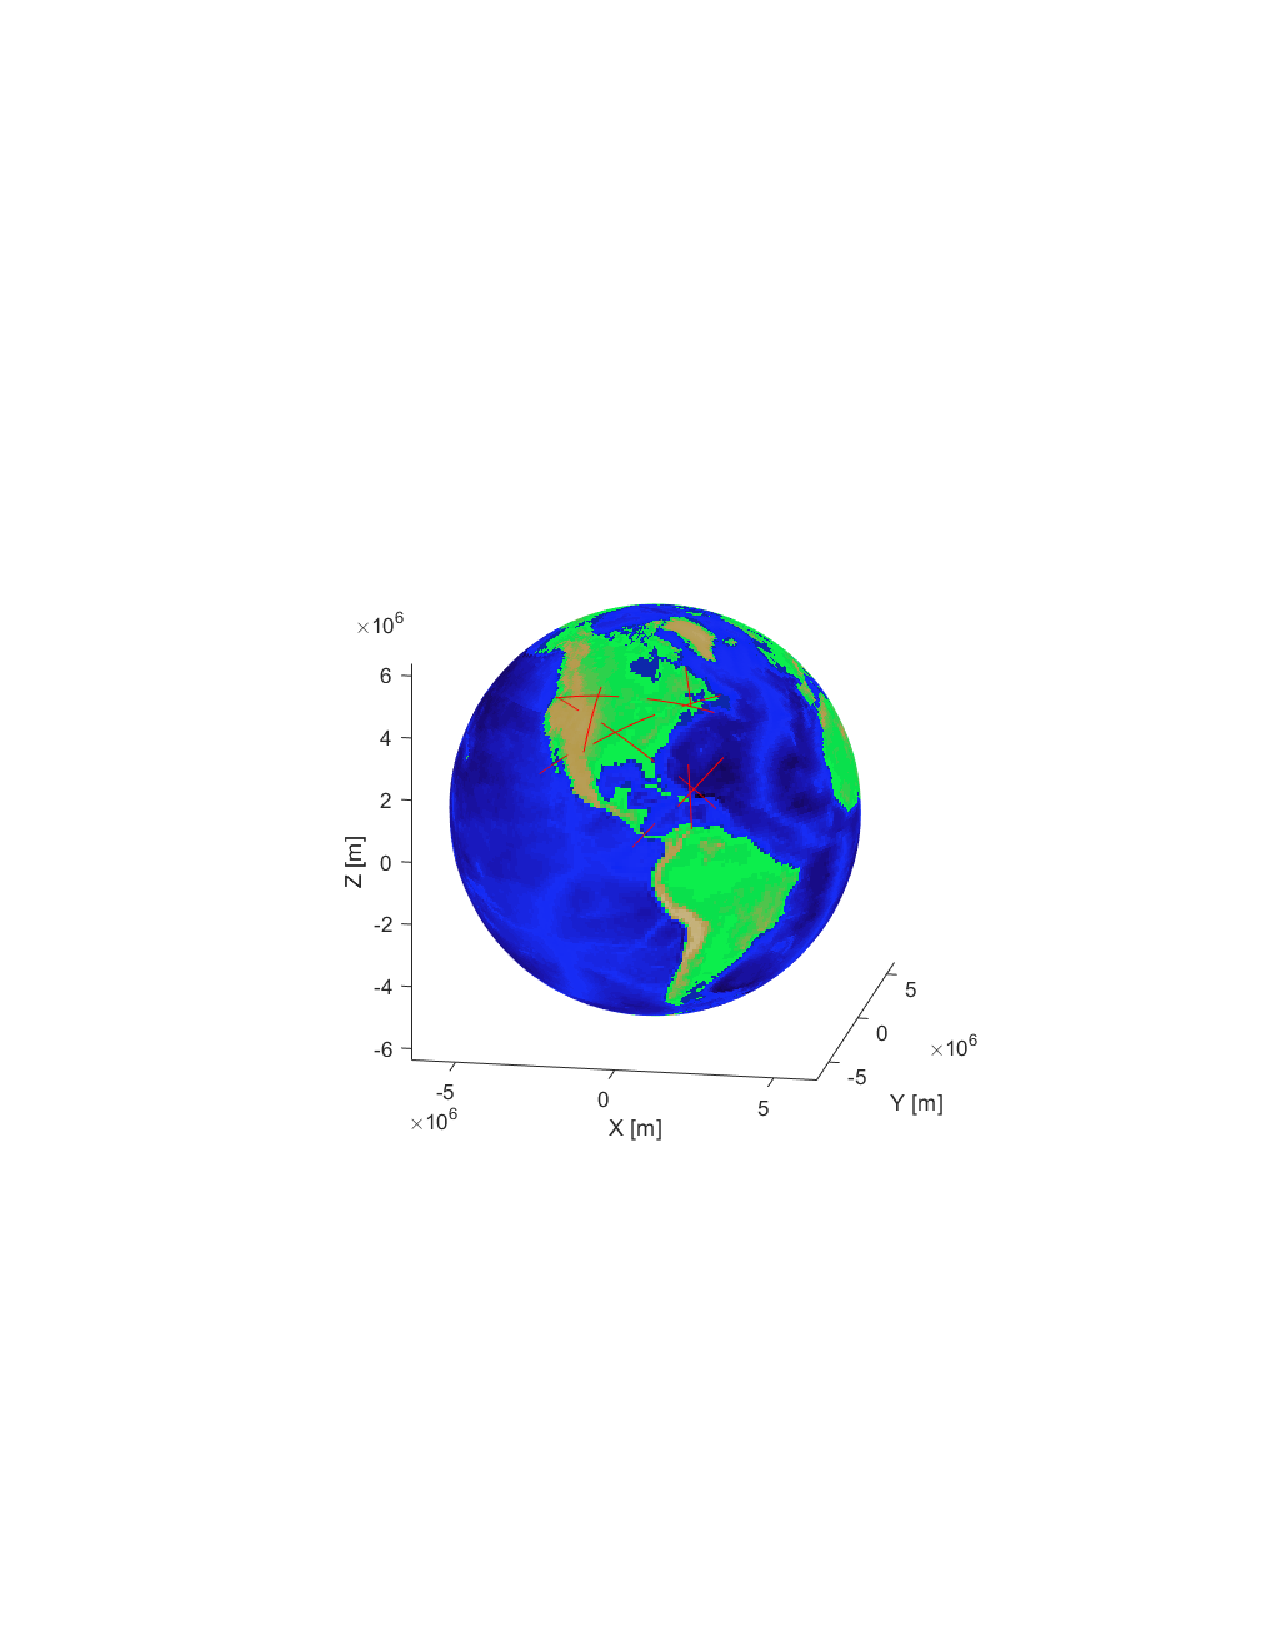
\includegraphics[trim=1.2in 3.3in 1.75in 3.3in,clip,width=5in]
    {Augment_Globe.pdf}
    \caption{Generated Augmented Satellite Constellation}
    \label{fig:AugmentGlobe}
\end{figure}

Figure \ref{fig:AugmentSky} shows the skyplot of the augmented satellites over the period of the simulation. 

\begin{figure}[h!]
    \centering
    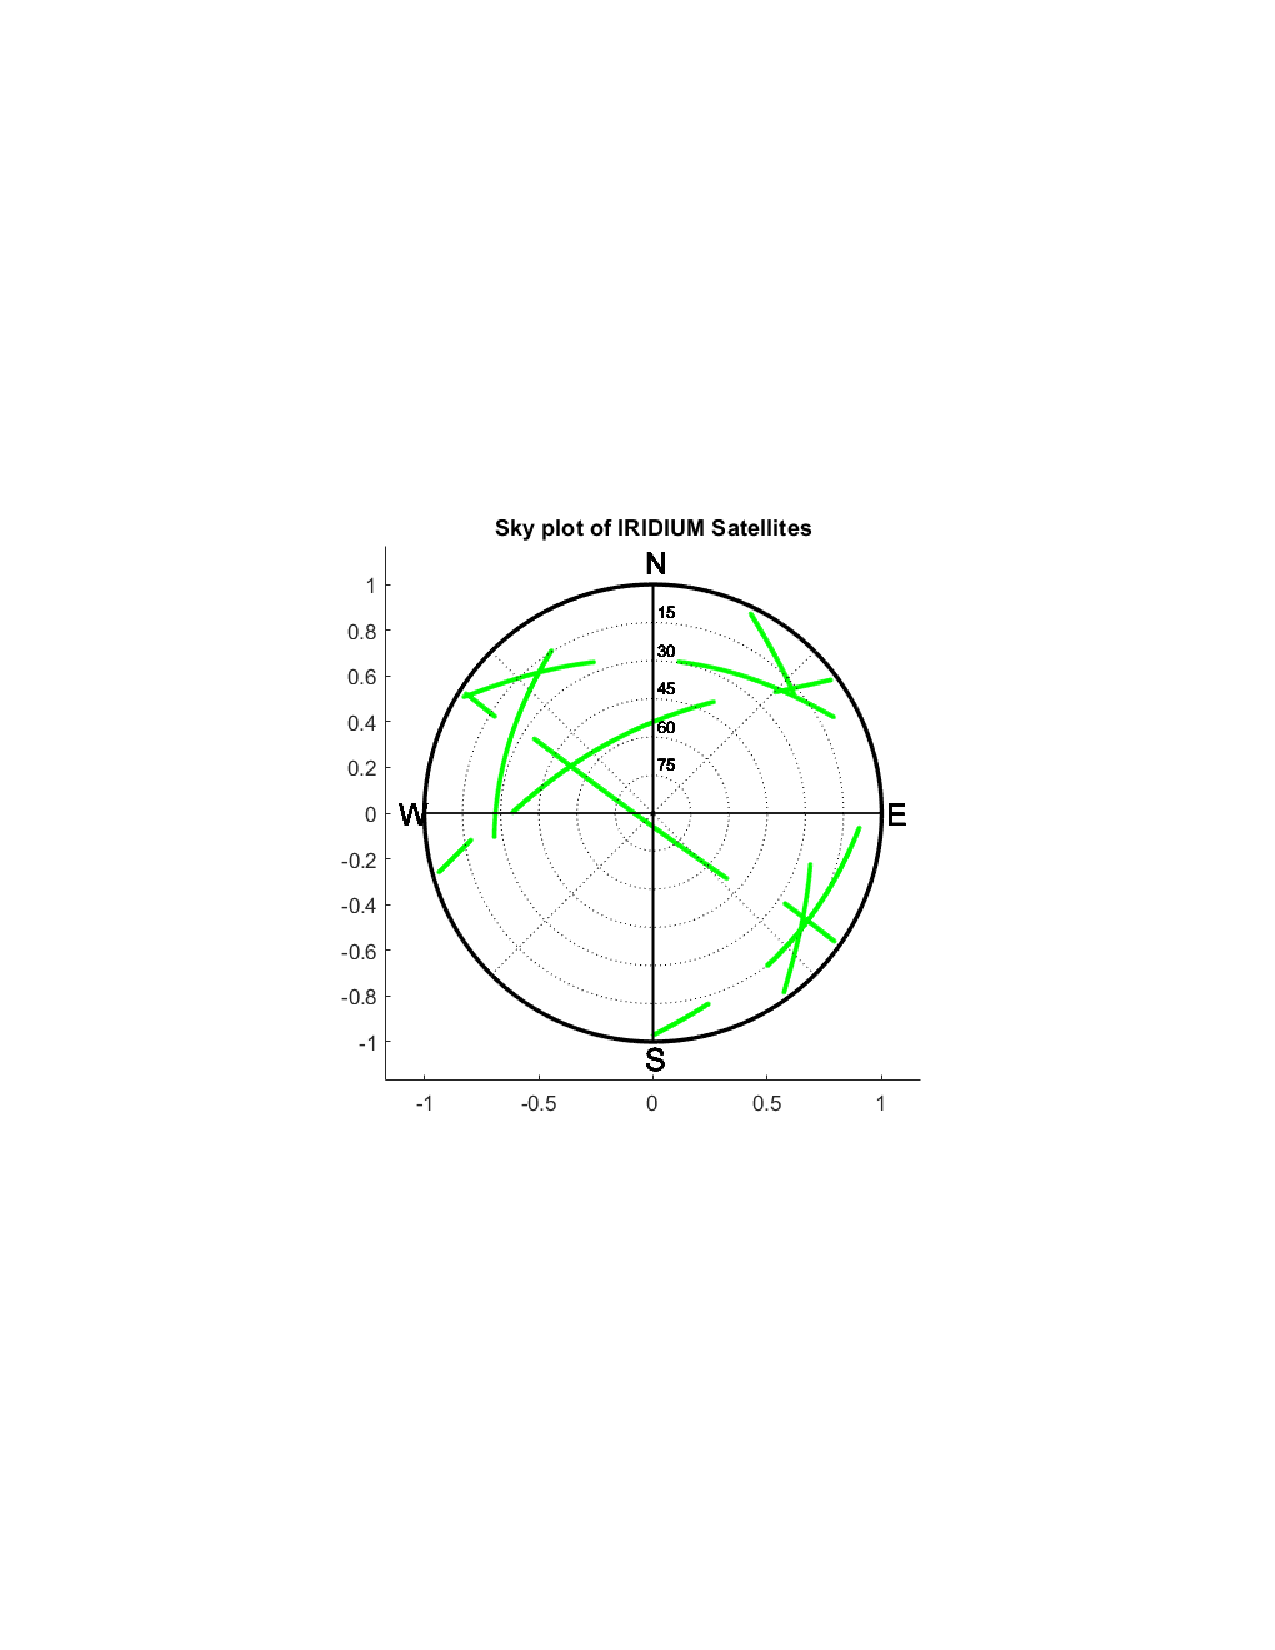
\includegraphics[trim=1.2in 3.3in 1.75in 3.7in,clip,width=5in]
    {Augment_Skyplot.pdf}
    \caption{Skyplot of Augmented Constellation}
    \label{fig:AugmentSky}
\end{figure}
\pagebreak

\subsection{Doppler Positioning}
The same Doppler positioning technique is used for this example. Figure \ref{fig:Augmentdopplerposit} shows the estimated receiver positions. It can be seen that the grouping of receiver estimates seems to be biased by around 1000 meters. One possible reason for this is that the satellite positions do not favor the southwest area of the sky seen by the near empty quadrant in \ref{fig:AugmentSky}. 

\begin{figure}[h!]
    \centering
    \includegraphics[trim=1.2in 3.3in 1.75in 3.3in,clip,width=5in]
    {Augment_5min_Doppler_posit.pdf}
    \caption{Doppler Position Estimates of Augmented Satellites}
    \label{fig:Augmentdopplerposit}
\end{figure}

The constant bias can be seen in Figure \ref{fig:AugmentdopplerRMSE}. The positioning error is most likely also caused by the error induced by the software receiver. 
\begin{figure}[h!]
    \centering
    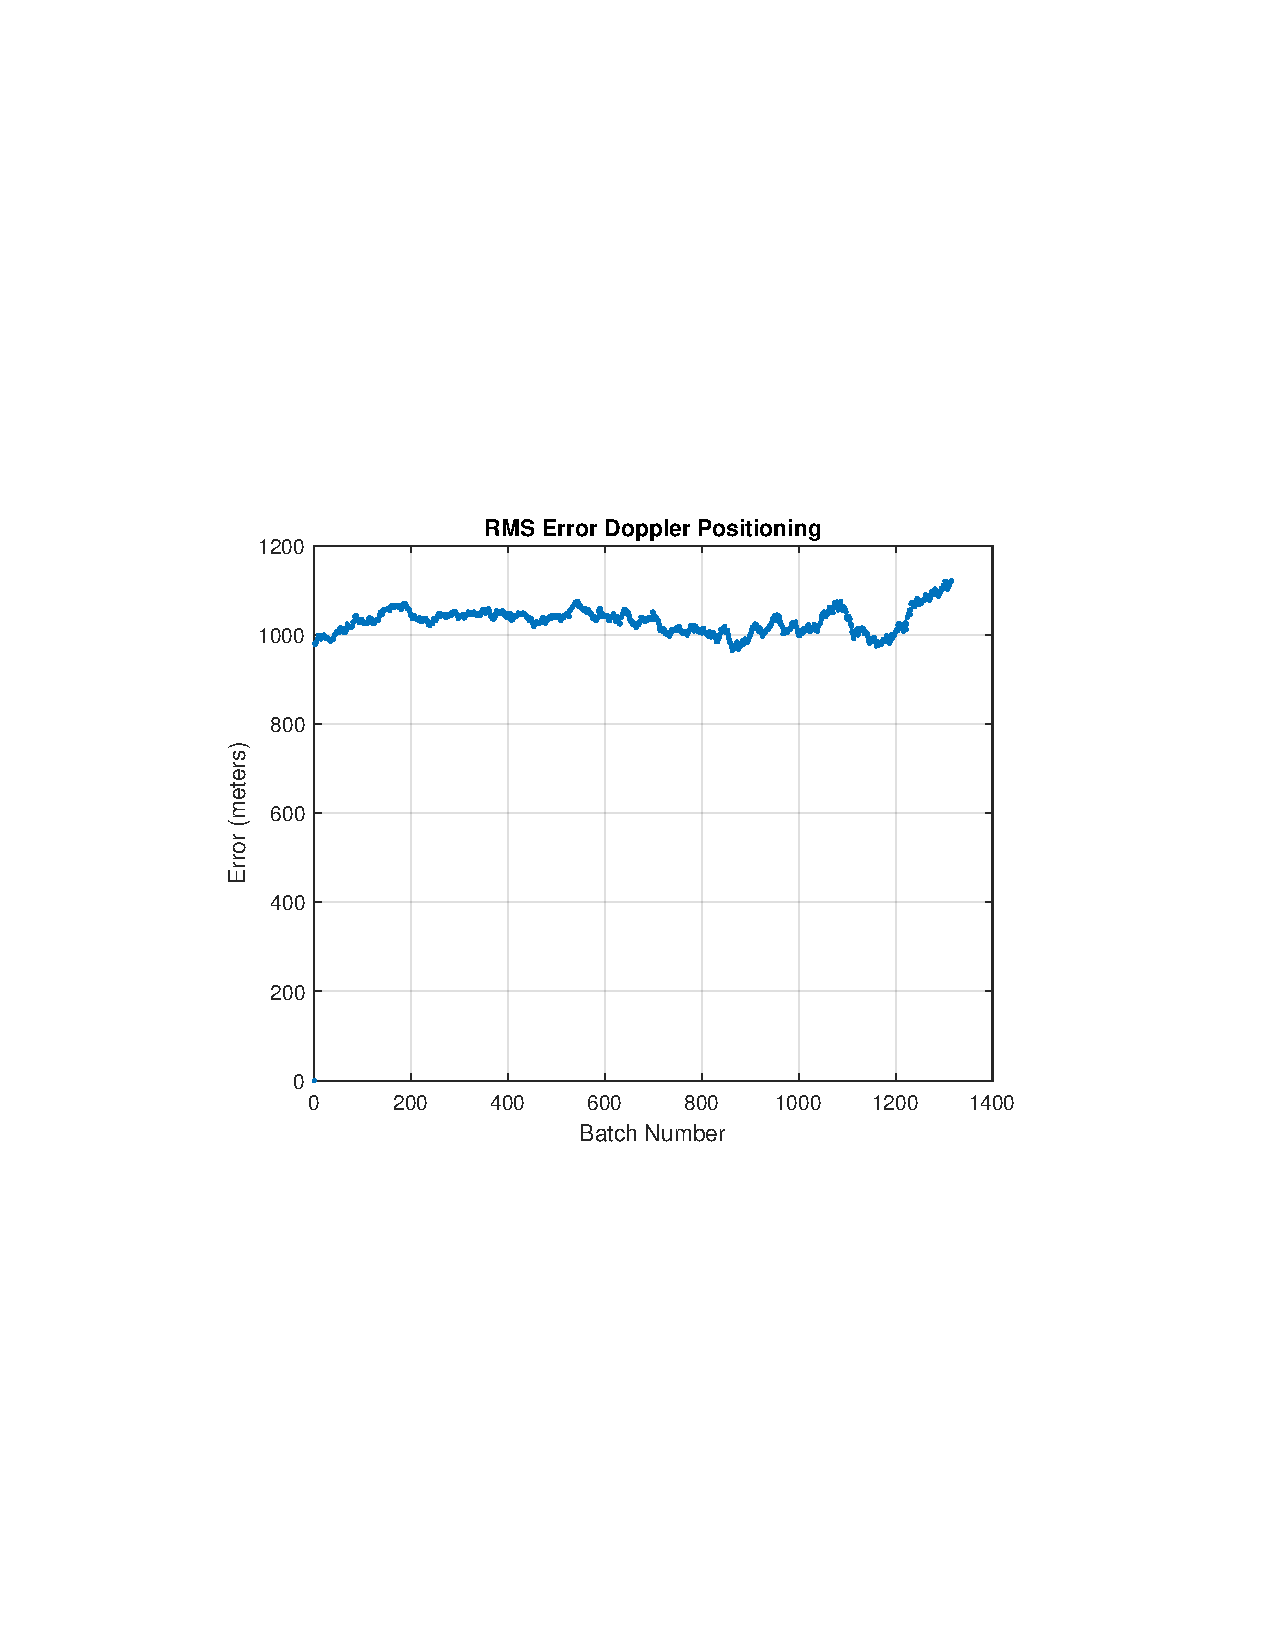
\includegraphics[trim=1.2in 3.3in 1.75in 3.3in,clip,width=5in]
    {Augment_5min_Doppler_RMSE.pdf}
    \caption{RMS Error Doppler Position Estimates of Augmented Satellites}
    \label{fig:AugmentdopplerRMSE}
\end{figure}
Figure \ref{fig:AugmentdopplerPDOP} shows the PDOP of each batched measurement. With the addition of more satellites, the PDOP fluctuates less and is the best of all simulations shown in this thesis. By adding more diversity to the satellites, the PDOP improves. While this is still not a GPS quality PDOP, it is more stable than the PDOP of the IridiumNext constellation.
\begin{figure}[h!]
    \centering
    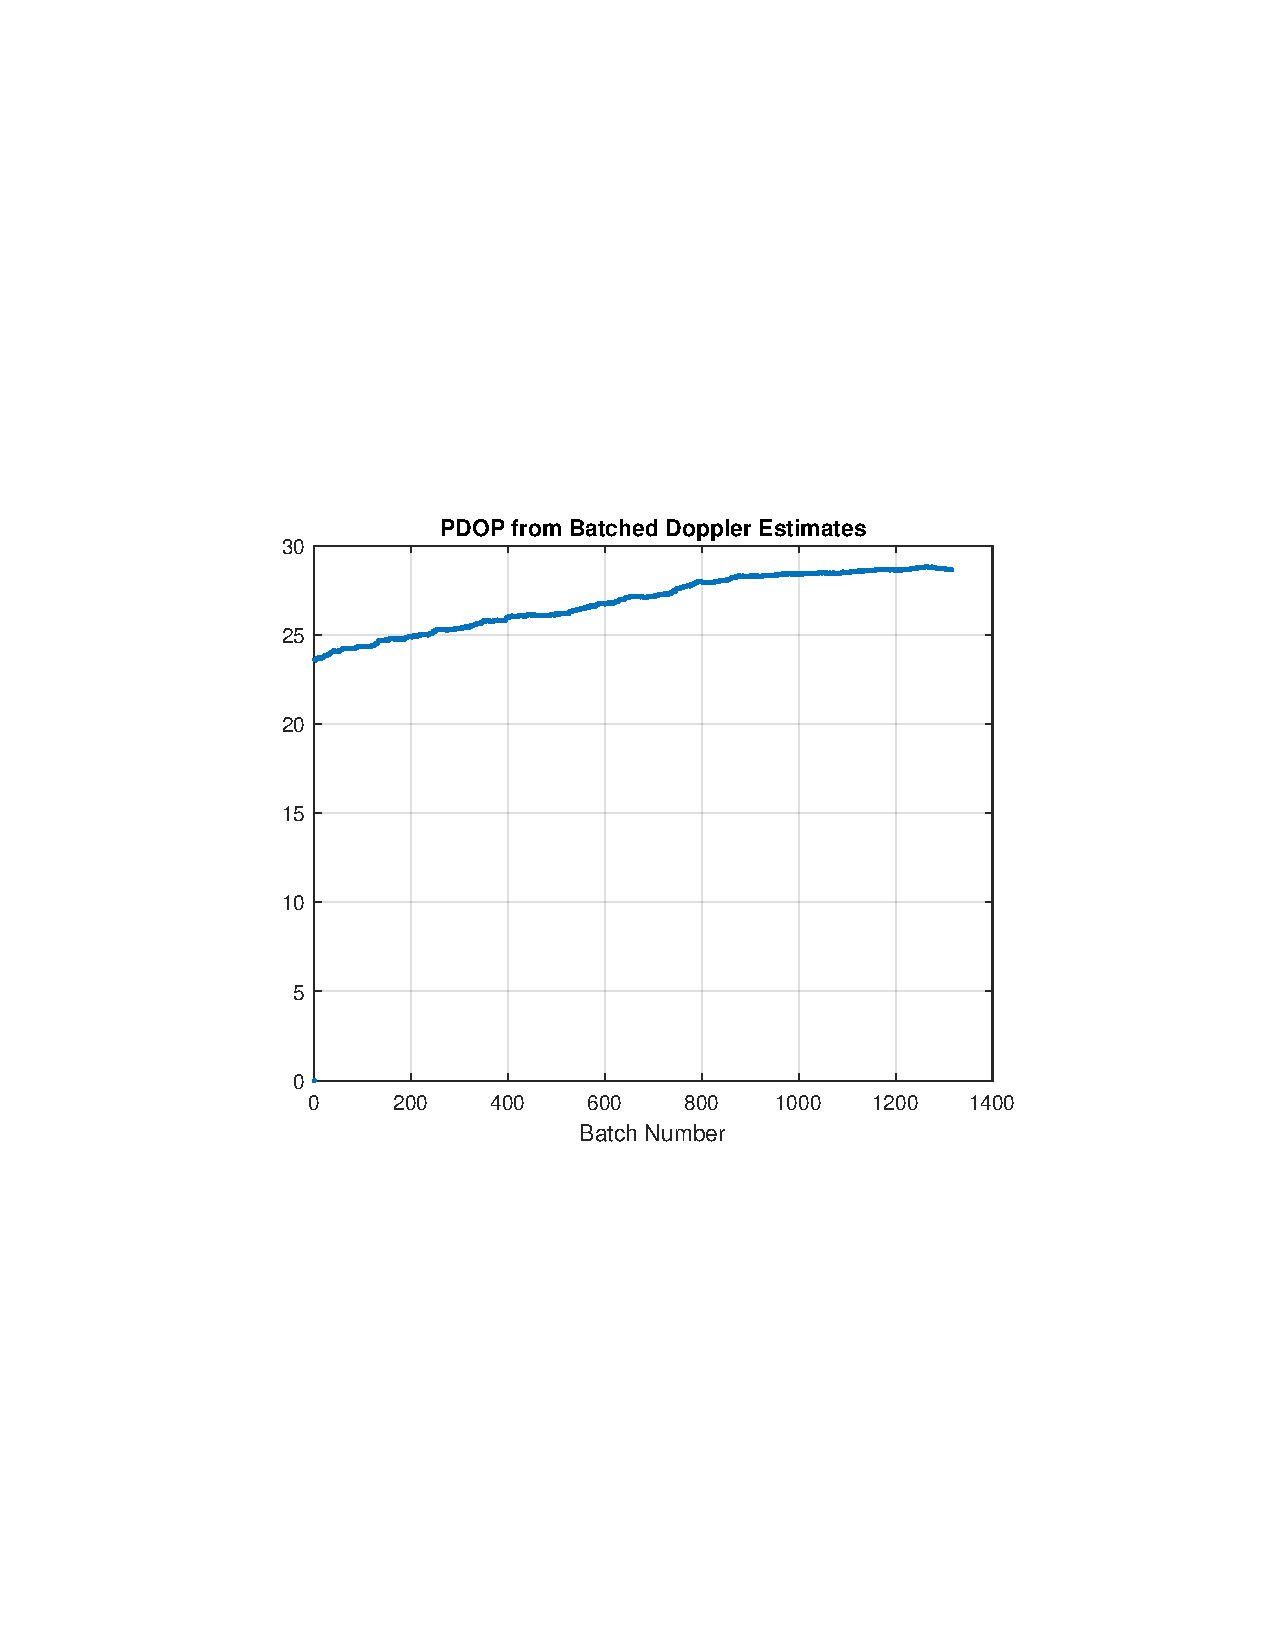
\includegraphics[trim=1.2in 3.3in 1.75in 3.3in,clip,width=5in]
    {Augment_5min_Doppler_PDOP.pdf}
    \caption{PDOP of Doppler Position Estimates of Augmented Satellites}
    \label{fig:AugmentdopplerPDOP}
\end{figure}

\pagebreak
\subsection{Pseudorange Based Positioning}
The pseudorange based positioning estimates are shown in Figure \ref{fig:Augmentpseudoposit}. While there are more position estimates in the Doppler solution, the RMS error is better in the pseudorange solution.
\begin{figure}[h!]
    \centering
    \includegraphics[trim=1.2in 3.3in 1.75in 3.3in,clip,width=5in]
    {Augment_5min_pseudo_posit.pdf}
    \caption{Pseudorange Position Estimates of Augmented Satellites}
    \label{fig:Augmentpseudoposit}
\end{figure}
The RMS error is shown in \ref{fig:AugmentpseudoRMSE}. The error is lower than in any of the previous simulations. The error in the pseudorange is most likely caused by the low resolution caused by the low sampling frequency. 

\begin{figure}[h!]
    \centering
    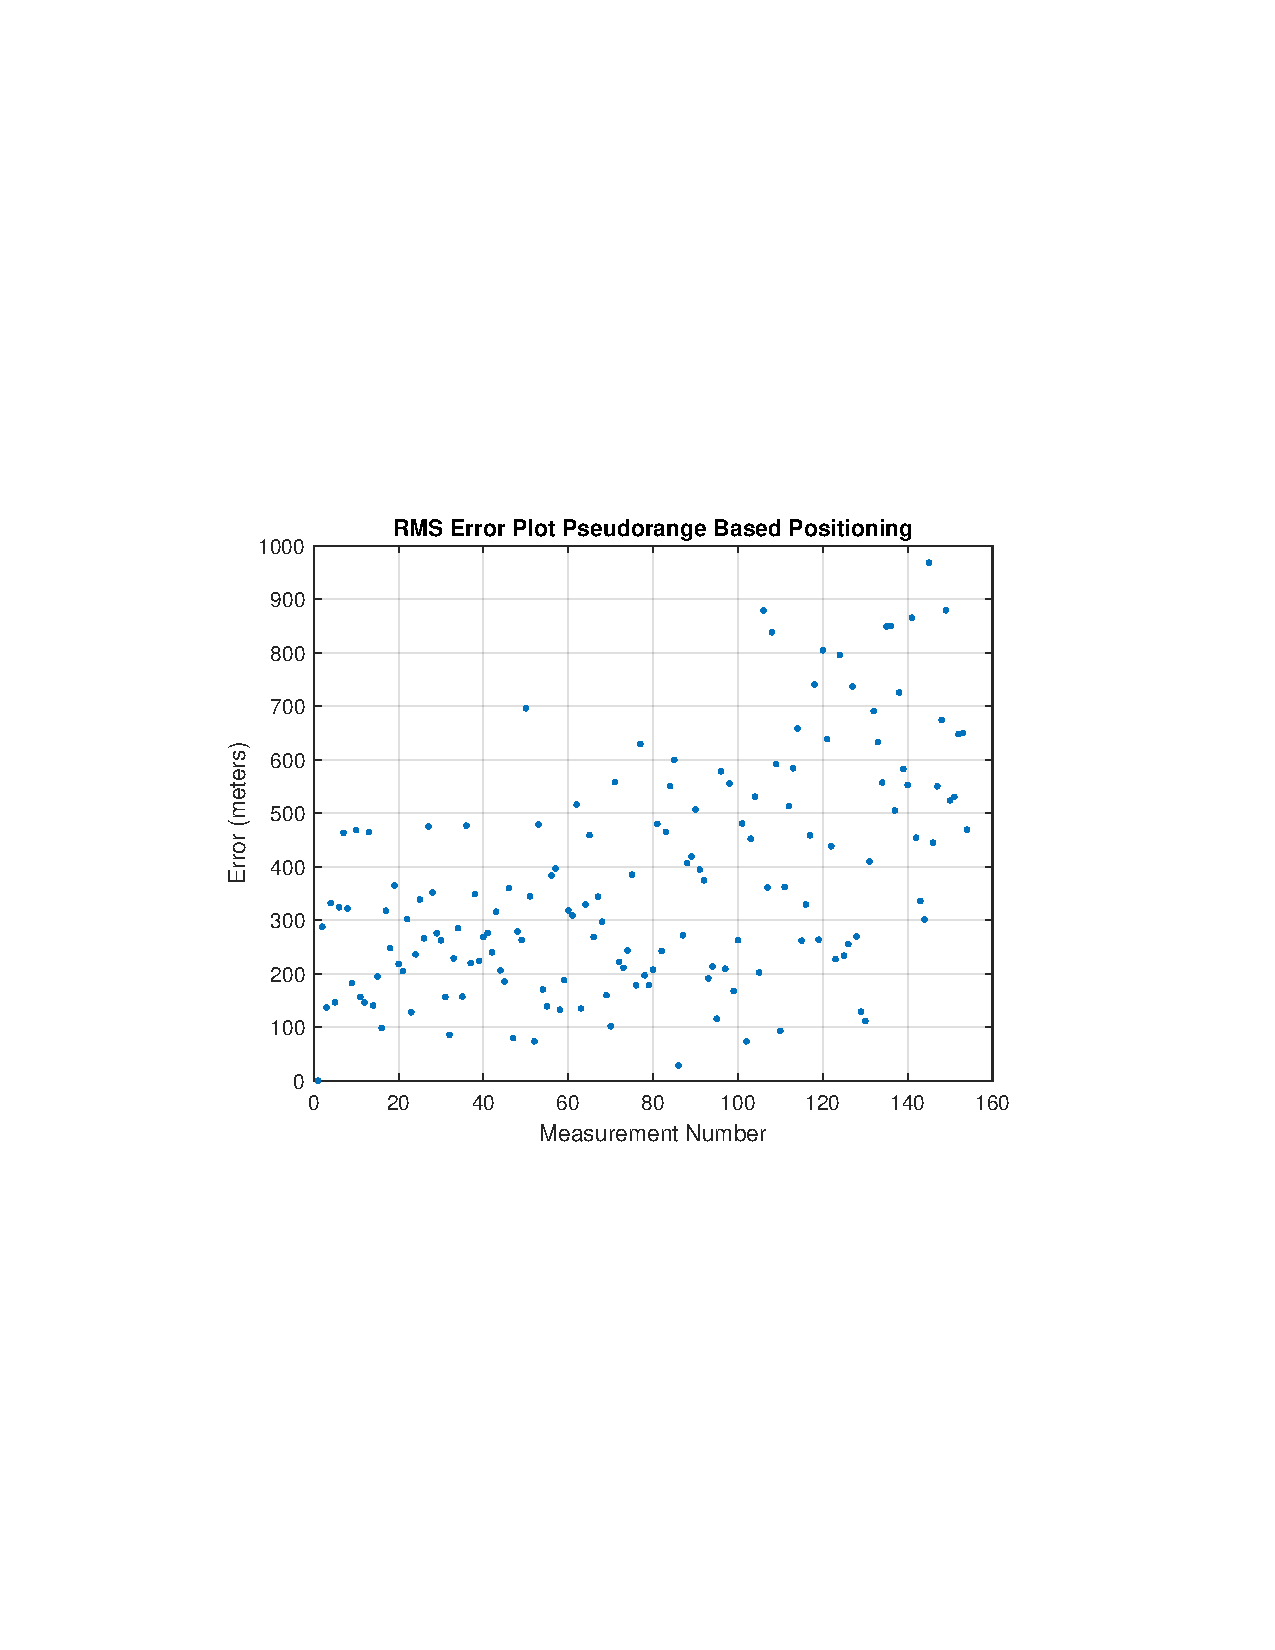
\includegraphics[trim=1.2in 3.3in 1.75in 3.3in,clip,width=5in]
    {Augment_5min_pseudo_RMSE.pdf}
    \caption{RMS Error of Pseudorange Position Estimates of Augmented Satellites}
    \label{fig:AugmentpseudoRMSE}
\end{figure}
Figure \ref{fig:AugmentpseudoPDOP} shows that the increased number of satellites has improved the PDOP from the IridiumNext simulation. 
\begin{figure}[h!]
    \centering
    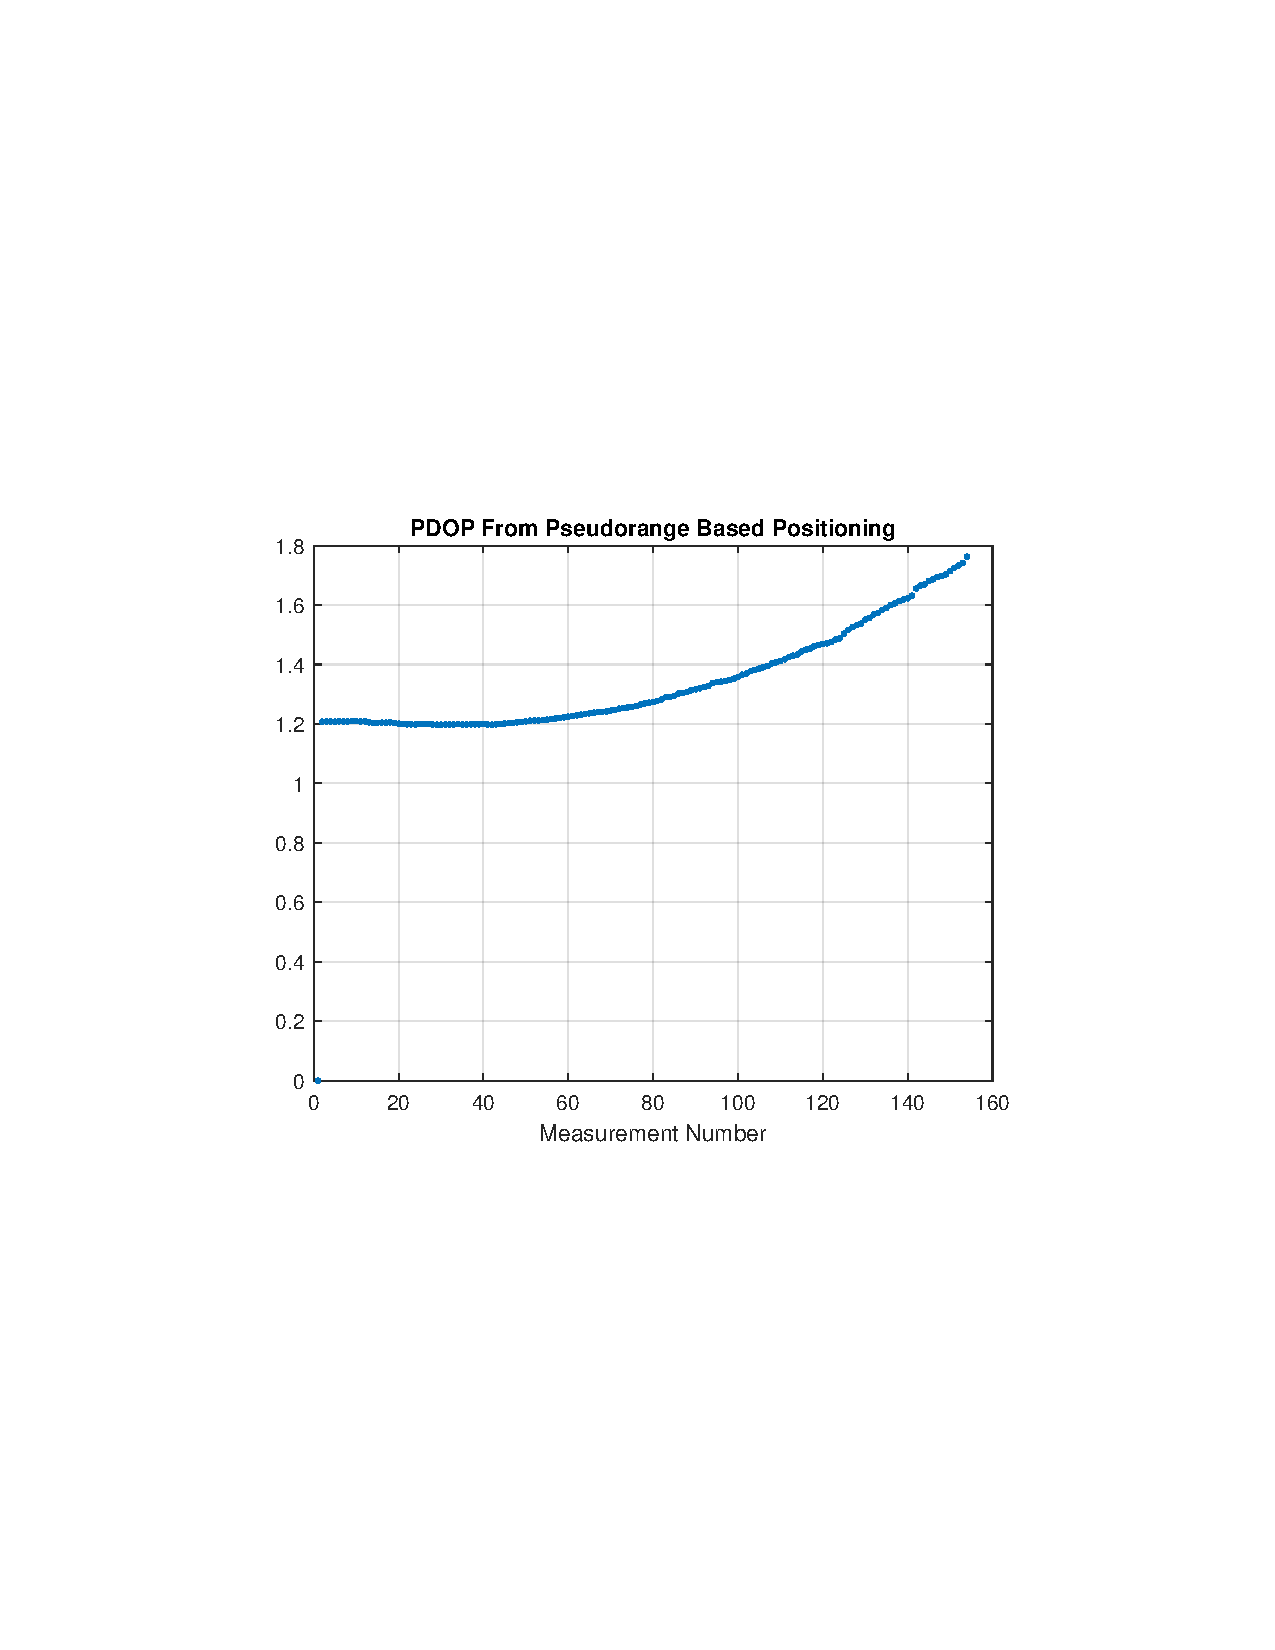
\includegraphics[trim=1.2in 3.3in 1.75in 3.3in,clip,width=5in]
    {Augment_5min_pseudo_PDOP.pdf}
    \caption{PDOP of Pseudorange Position Estimates of Augmented Satellites}
    \label{fig:AugmentpseudoPDOP}
\end{figure}
Overall, the increased number of satellites has improved the positioning estimate. This is expected as more satellites result in an increased number of measurements and an increased diversity of satellite locations. 

\pagebreak
\section{Dynamic Clean Data}
Another capability of this simulator is the ability to generate data for dynamic trajectories. For a dynamic trajectory simulation, the user will begin by setting the user position and velocity to a predetermined path. The position and velocity will be in the ECEF coordinate frame. The data set used for this test was taken by driving a path with a Lincoln MKZ that had an eTalin measurement device. A plot of the path driven is shown below in Figure \ref{fig:Dynamicpath}

\begin{figure}[h!]
    \centering
    \includegraphics[trim=1.2in 3.3in 1.75in 3.3in,clip,width=5in]
    {Dynamic_Etalin_PlotDriven.pdf}
    \caption{Path Driven for Dynamic Data}
    \label{fig:Dynamicpath}
\end{figure}

The positioning techniques used in this thesis are not applicable to dynamic receivers. This is because they require batched measurements to calculate a position. A positioning solution will not be calculated for the dynamic test. To show an output of the simulation, the received Doppler frequency of the generated signal will be compared against Doppler measurements from a Jackson Labs receiver. The Jackson Labs receiver is an Iridium specific receiver for the satellite timing and location (STL) signal. Figure \ref{fig:gendynamdop} shows the generated Doppler frequencies for the dynamic test. Figure \ref{fig:JLdynamdop} shows the live sky received Doppler frequencies from the Jackson Labs receiver.

\begin{figure}[h!]
    \centering
    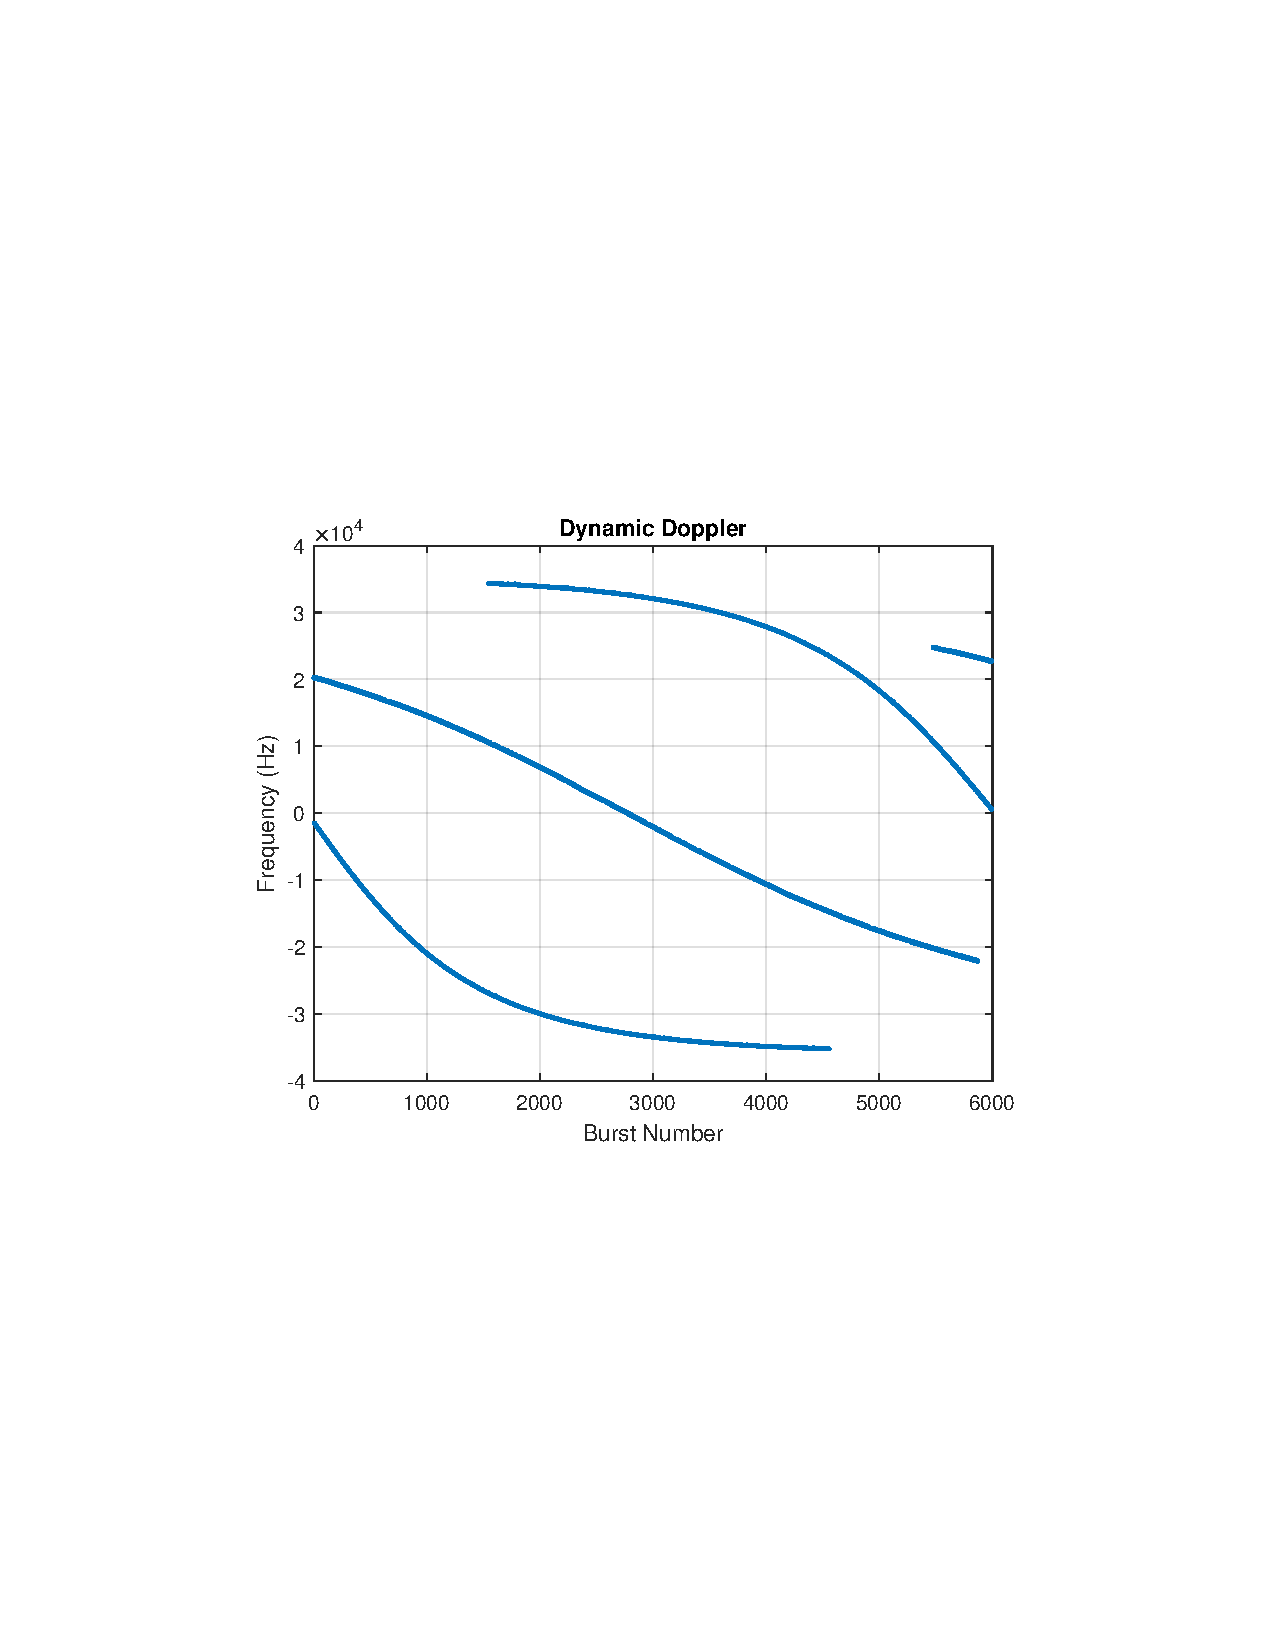
\includegraphics[trim=1.2in 3.3in 1.75in 3.3in,clip,width=5in]
    {Dynamic_Irid_Doppler-2.pdf}
    \caption{Generated Dynamic Doppler Measurements}
    \label{fig:gendynamdop}
\end{figure}

\begin{figure}[h!]
    \centering
    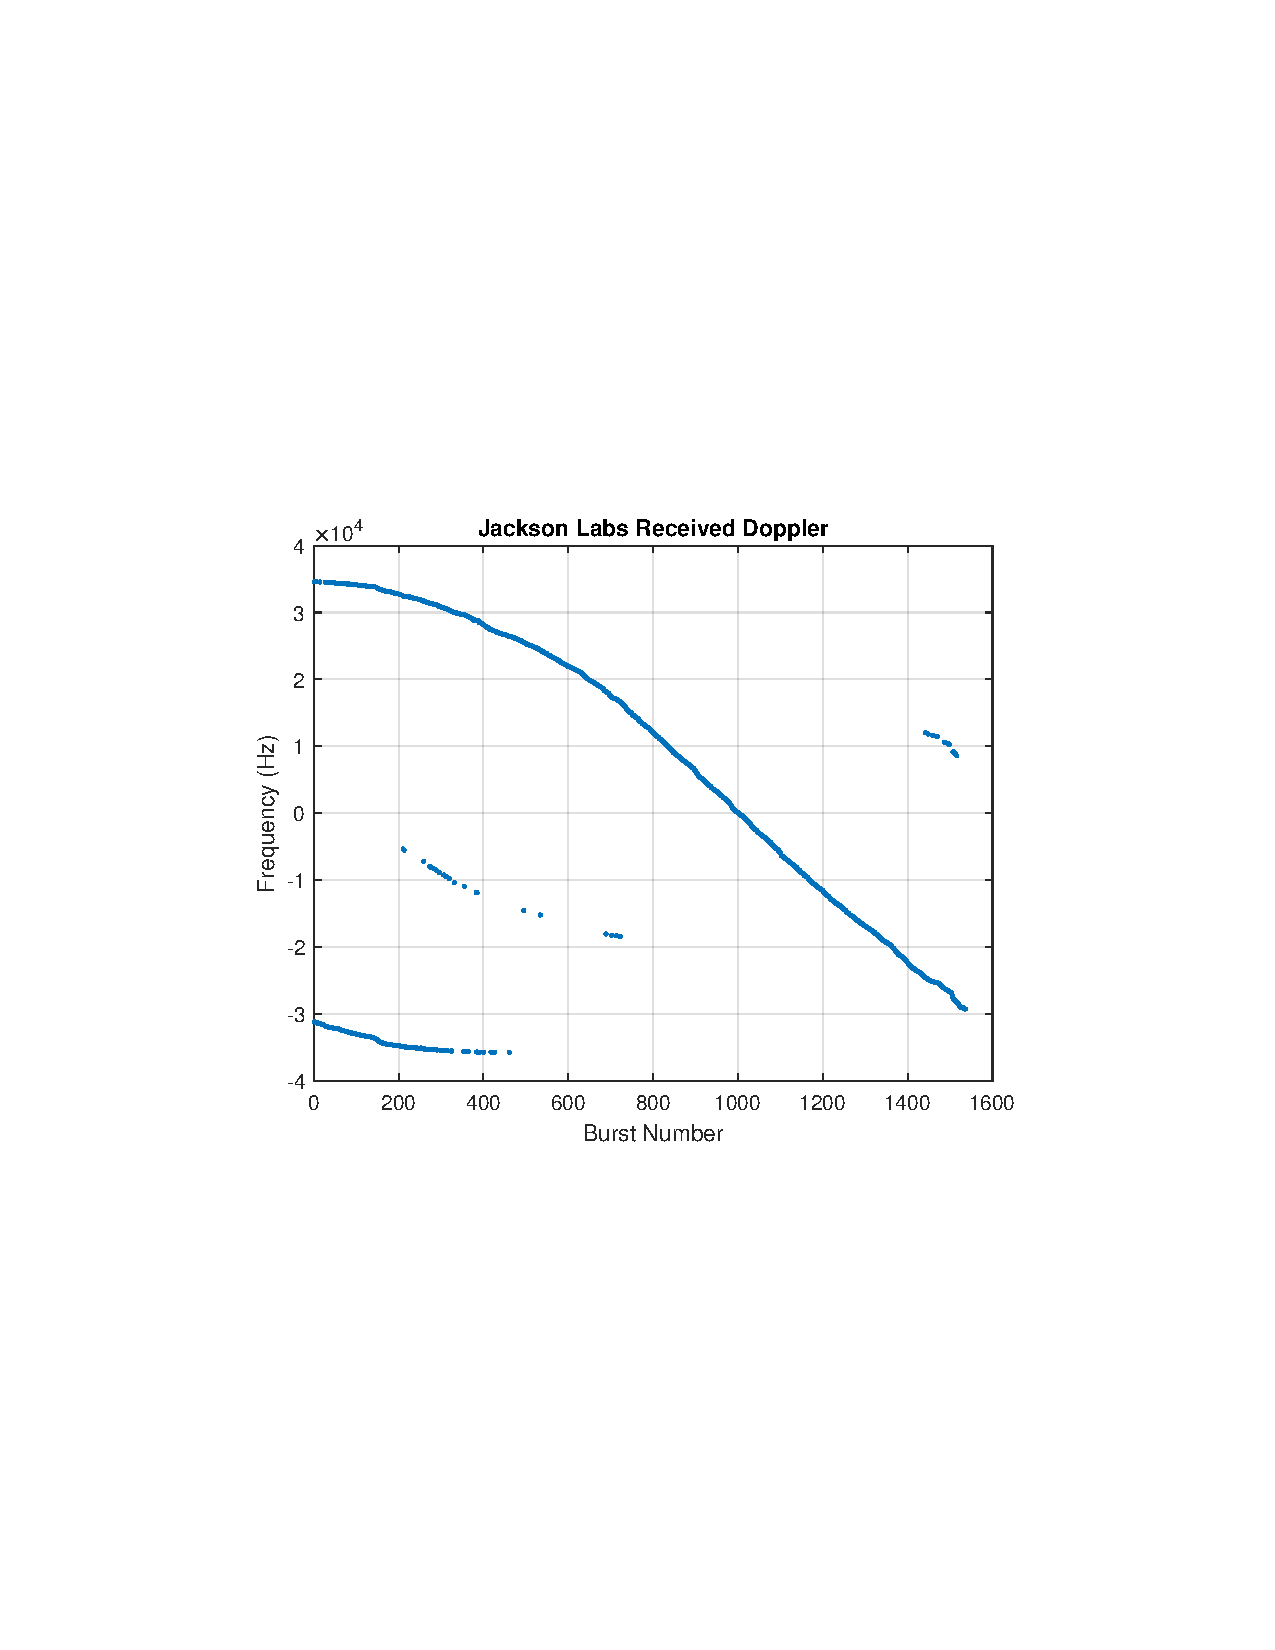
\includegraphics[trim=1.2in 3.3in 1.75in 3.3in,clip,width=5in]
    {Dynamic_JL_Doppler-2.pdf}
    \caption{Jackson Labs Doppler Measurements}
    \label{fig:JLdynamdop}
\end{figure}

It was important to synchronize the simulation time with the actual time of the data run to accurately simulate the satellites that were in view at the time of the data collection. Even with synchronizing the time of simulation to the data collection, the simulated satellite positions were not accurate to the live sky data. Also, the assumption in this simulation tool is that the receiver will receive a burst at each interval. In the real world this is not the case. There is a larger mask angle from satellites in the real world due to buildings, trees, and landscape. This decreases the number of bursts received by the receiver. 

The purpose of this experiment was to prove that a signal could be calculated for a dynamic data set. While the receiver position could not be estimated, the output and comparison of Doppler frequencies shows that the simulator is capable of generating a signal for a dynamic trajectory and successfully receive the data.  

\chapter{Conclusions and Future Work}
\section{Summary}
Chapter 1 discusses the motivation behind this thesis and why there is a need for a LEO satellite signal simulation tool. Having a simulation tool to test current and hypothetical signals and satellite constellations for investigative purposes is important in the engineering process. Before hardware is developed or satellites are launched, the constellation and signals need to be tested in software. Testing in software allows for changes to be made in the development process where the cost of changes are minimal. Once satellites are launched and hardware has been assembled, the margin to change is thin. Simulation tools allow for fast testing and validation of techniques and algorithms. This simulation in particular aids the engineering process by being able to generate signals for satellite constellations that can be processed through software and hardware receivers. This chapter also discusses prior work with LEO satellites and GNSS signal simulators. Most of the prior work is aimed at using LEO satellites as signals of opportunity to aid navigation solutions in areas of poor GNSS reception. This is followed by the contributions of this thesis and an outline. 

Chapter 2 begins with a brief introduction to satellite based navigation where trilateration is introduced. This is followed by describing different orbit zones around the Earth and what satellites occupy that specific space. Next channel access methods such as TDMA, CDMA, and FDMA are mentioned in brief. Chapter 2 is concluded by mentioning different modulation techniques. 

Chapter 3 discusses the simulation tool in parts. It begins by giving an overview of the entire simulation process. Next the simulation settings are defined along with all of the terms the user can change. The measurement simulation is discussed fully where the inputs and outputs are explained and what their purpose is later in the simulation. The mathematical calculation of measurements are also given in this section. The process of generating the signal is discussed. Finally, the receiver used in this thesis is described.

Chapter 4 defines the testing setup and positioning techniques. In this thesis, multiple different simulations were conducted to show the versitility of the tool. The testing setup is mainly in software, but there is the introduction of a USRP to show the generated signal has the ability to be played into hardware. The positioning techniques used in this thesis are batched Doppler and a pseudorange least squares estimation.

Chapter 5 provides the positioning results of the output signal data. Geographical plots of the position estimates, RMS error, and PDOP are used to show how the outputs of the signal are used. This is the validation that the generated signal could be used for navigation and that the generated signal is real. 

\section{Conclusions}
This thesis developed a simulation tool capable of generating navigation signals for LEO satellites. The simulation tool works well for its purpose. It has shown the ability to generate realistic IQ data for LEO satellites. The ability to test different constellation configurations, signal types, data messages, error types, and other settings is vital. This thesis has accomplished making contributions in the field of navigation. A comprehensive simulation tool for generating measurements and signals for LEO satellites was developed. The signal showed that it could be played through a software receiver and a USRP. Positioning techniques for a TDMA signal were used to validate the signal. While the positioning results are not as robust as GNSS standards, the navigation data was proven to provide a positioning solution. 


\section{Future Work}
The future work for this project can take the direction of making additions to the simulation tool. The addition of multiple signal types would be beneficial as new and emerging satellite constellations will need to be simulated. A modular software receiver tied directly to the signal simulation would make the process of receiving the signal more streamline. The addition of more error terms, such as ionospheric error would improve the quality of the simulation tool. Another piece could be the addition of a clock model that more accurately describes the nature of clocks used in satellites and receivers. With new emerging satellite constellations such as Starlink and Xona, the addition of those satellite constellations and signals could be an avenue to pursue. 

More future work could include developing a hardware receiver for a specific receiver to test the capability of this simulation tool. It could be interesting to see how this signal simulation would work with a hardware in the loop (HWIL) simulation. For an HWIL project, a predetermined signal type and data message structure would need to be decided before work on the hardware could begin. Once the signal had been decided upon, the user could begin rearanging the simulation tool to match the desired signal. 

Futher expansion of this thesis is to develope a more rigorous navigation message. While the navigation message in this thesis works, the introduction of a higher fidelity satellite propagation model will require more terms to account for corrections. Also, the addition of more positioning techniques as forms of colaborative navigation could be interesting to investigate. 


\bibliographystyle{unsrt}
\bibliography{MyLibrary}
%\bibliography{export-data-2}





%\begin{appendix}
%\chapter*{Appendices\addcontentsline{toc}{chapter}{Appendices}}


%\begin{singlespace}


%\end{singlespace}
%\end{appendix}
\end{document}

